% mnras_template.tex 
%
% LaTeX template for creating an MNRAS paper
%
% v3.0 released 14 May 2015
% (version numbers match those of mnras.cls)
%
% Copyright (C) Royal Astronomical Society 2015
% Authors:
% Keith T. Smith (Royal Astronomical Society)

% Change log
%
% v3.0 May 2015
%    Renamed to match the new package name
%    Version number matches mnras.cls
%    A few minor tweaks to wording
% v1.0 September 2013
%    Beta testing only - never publicly released
%    First version: a simple (ish) template for creating an MNRAS paper

%%%%%%%%%%%%%%%%%%%%%%%%%%%%%%%%%%%%%%%%%%%%%%%%%%
% Basic setup. Most papers should leave these options alone.
\documentclass[fleqn,usenatbib]{mnras}

% MNRAS is set in Times font. If you don't have this installed (most LaTeX
% installations will be fine) or prefer the old Computer Modern fonts, comment
% out the following line
\usepackage{newtxtext,newtxmath}
% Depending on your LaTeX fonts installation, you might get better results with one of these:
%\usepackage{mathptmx}
%\usepackage{txfonts}

% Use vector fonts, so it zooms properly in on-screen viewing software
% Don't change these lines unless you know what you are doing
\usepackage[T1]{fontenc}
\usepackage{ae,aecompl}




%%%%% AUTHORS - PLACE YOUR OWN PACKAGES HERE %%%%%

% Only include extra packages if you really need them. Common packages are:
\usepackage{graphicx}	% Including figure files
\usepackage{amsmath}	% Advanced maths commands
\usepackage{amssymb}	% Extra maths symbols
\usepackage{braket}
\usepackage{siunitx} %v. useful units package 
\usepackage{multirow}
\usepackage{mathtools}
\usepackage{makecell}
\renewcommand{\cellalign}{l}
% \usepackage{caption}
\usepackage[caption = false]{subfig}
% \usepackage{subcaption}
% \captionsetup{compatibility=false}
% \usepackage{subfigure}
% \usepackage{mwe}
\usepackage{multirow}
\usepackage{ulem}
%%%%%%%%%%%%%%%%%%%%%%%%%%%%%%%%%%%%%%%%%%%%%%%%%%
\usepackage{float}
\restylefloat{table}
% \usepackage[mathlines]{lineno}
\usepackage{lineno}
\linenumbers

%%%%% AUTHORS - PLACE YOUR OWN COMMANDS HERE %%%%%

% Please keep new commands to a minimum, and use \newcommand not \def to avoid
% overwriting existing commands. Example:
%\newcommand{\pcm}{\,cm$^{-2}$}	% per cm-squared
\newcommand{\xip}{\ensuremath{\xi_{+}}}
\newcommand{\xim}{\ensuremath{\xi_{-}}}
\newcommand{\xipm}{\ensuremath{\xi_{\pm}}}
\newcommand{\gammat}{\ensuremath{\gamma_{\rm t}(\theta)}}
\newcommand{\wtheta}{\ensuremath{w(\theta)}}
\newcommand{\dsigr}{\ensuremath{\Delta\Sigma(R)}}
\newcommand{\dsigobsr}{\ensuremath{\Delta\Sigma^{\mathrm{obs}}(R)}}
\newcommand{\dsigmodr}{\ensuremath{\Delta\Sigma^{\mathrm{model}}(R)}}

\newcommand{\pgg}{\ensuremath{P_{\mathrm{gg}}}}
\newcommand{\pgm}{\ensuremath{P_{\mathrm{gm}}}}
\newcommand{\xigg}{\ensuremath{\xi_{\mathrm{gg}}} }
\newcommand{\xigm}{\ensuremath{\xi_{\mathrm{gm}}} }

\DeclareMathAlphabet\mathbfcal{OMS}{cmsy}{b}{n}


%units
\DeclareSIUnit \megaparsec {Mpc}
\DeclareSIUnit \h {\mbox{$h$}}

%cosmo parameters
\newcommand{\om}{\ensuremath{\Omega_{\mathrm m}}}
\newcommand{\ol}{\Omega_{\mathrm \Lambda}}
\newcommand{\omb}{\Omega_{\mathrm b}}
\newcommand{\sig}{\ensuremath{\sigma_8}}
\newcommand{\lcdm}{$\Lambda$CDM}
\newcommand{\wcdm}{$w$CDM}
\newcommand{\ns}{n_s}
\newcommand{\w}{w_0}
\newcommand{\wa}{w_a}

% eqn and figures
\newcommand\eqn[1]{equation~\ref{#1}}
\newcommand\eqnb[2]{equations~\ref{#1}~\& \ref{#2}}
\newcommand\eqnc[2]{equations~\ref{#1}--\ref{#2}}
\newcommand\Eqn[1]{Equation~\ref{#1}}   % If you need to start a sentence with this...
\newcommand\Eqnb[2]{Equations~\ref{#1}~\& \ref{#2}}

% Likewise for figures and tables
\newcommand\fig[1]{Figure~\ref{#1}}
\newcommand\figb[2]{Figures~\ref{#1}~\& \ref{#2}}
\newcommand\chap[1]{Chapter~\ref{#1}}
\newcommand\sect[1]{Section~\ref{#1}}
\newcommand\tab[1]{Table~\ref{#1}}
\newcommand\app[1]{Appendix~\ref{#1}}
\newcommand{\redmagic}{\texttt{redMaGiC} }
\newcommand{\mice}{\texttt{MICE} }
\newcommand{\maglim}{\texttt{MagLim} }
\newcommand{\gold}{\texttt{GOLD} }
\newcommand{\buzzard}{\texttt{Buzzard} }

\newcommand{\hinv}{h^{-1}}
\newcommand{\beq}{\begin{equation}}
\newcommand{\eeq}{\end{equation}}
\newcommand{\hfour}{\hspace{4pt}}
\newcommand{\htwo}{\hspace{2pt}}
\newcommand{\nhat}{\hat{\textbf{n}}}
\newcommand{\del}{\partial}
\newcommand{\Chi}{\mathcal{X}}
\newcommand{\mb}{\mathbf}
\newcommand{\CLASS}{\texttt {CLASS}}
\newcommand{\COSMOLIKE}{\texttt {CosmoLike}}
\newcommand{\Camb}{\texttt {\textsc{Camb}}}
\newcommand{\HEALPIX}{{\textsc{Healpix}}}
\newcommand{\Halofit}{{\texttt{Halofit}}}
\newcommand{\balrog}{{\textsc{Balrog}}}

\newcommand{\metacal}{{\textsc{Metacalibration}~}}
\newcommand{\ttt}{{$3\times2$-point}}
\newcommand{\twottwo}{{$2\times2$-point}}

\usepackage{xspace} %This allows to add extra space when needed in new commands

\newcommand{\sdir}{\textsc{3sDir}\xspace}

\newcommand{\Nsims}{{{18}}}
%\usepackage[bottom]{footmisc}
\renewcommand{\thefootnote}{\arabic{footnote}}


\newcommand{\WMAP}{{\slshape WMAP~}}
\newcommand{\LCDM}{$ \Lambda $CDM~}
\newcommand{\PLANCK}{{\slshape PLANCK~}}
\newcommand{\WMAPc}{{\slshape WMAP}}
\newcommand{\CMBFAST}{\texttt {cmbfast~}}
\newcommand{\LCDMc}{$ \tilde{\lambda} $CDM}
\newcommand{\Planck}{{\slshape Planck~}}
\newcommand{\Planckc}{{\slshape Planck}}
\newcommand{\fsz}{\ensuremath{f_{sz}^{150}}}
\newcommand{\mbl}{\ensuremath{\mathbf{l}}}
\newcommand{\addgals}{{\sc Addgals}}
\newcommand{\calclens}{{\sc Calclens}}
\newcommand{\buzzardtwo}{{\sc Buzzard v2.0}}
\newcommand{\kcorrect}{{\sc kcorrect}}

\newcommand{\msol}{\ensuremath{h^{-1}M_{\odot}}}
\newcommand{\Msol}{\ensuremath{M_{\odot}}}
\newcommand{\mpc}{\ensuremath{h^{-1}\mathrm{Mpc}}}
\newcommand{\gpc}{\ensuremath{h^{-1}\mathrm{Gpc}}}
\newcommand{\gpcc}{\ensuremath{h^{-3}\mathrm{Gpc}^3}}
\newcommand{\kpc}{\ensuremath{h^{-1}\mathrm{kpc}}}
\newcommand{\Mpc}{\mathrm{Mpc}}
\newcommand{\nbody}{$N$-body}

\newcommand{\cs}{\ensuremath{\xi_{\pm}}}
\newcommand{\seight}{\ensuremath{S_8}}


\newcommand{\SP}[1]{{\color{red}[SP: #1]}}
\newcommand{\Yv}[1]{{\color{blue}[YYY]}}
\newcommand{\brown}[1]{\textcolor{brown}{#1}}
\newcommand{\myvec}[1]{\hat{\mathbf{#1}}}
\newcommand{\jdr}[1]{{\color{blue}[JDR: #1]}}


\newcommand{\red}[1]{\textcolor{red}{#1}}
\newcommand{\blue}[1]{\textcolor{blue}{#1}}
\newcommand{\IR}[1]{{\color{red}[\textbf{Note for IR}: #1]}}



%%%%%%%%%%%%%%%%%%%%%%%%%%%%%%%%%%%%%%%%%%%%%%%%%%

%%%%%%%%%%%%%%%%%%% TITLE PAGE %%%%%%%%%%%%%%%%%%%

% Title of the paper, and the short title which is used in the headers.
% Keep the title short and informative.
\title[Short title, max. 45 characters]{DES Y3 results: Constraints on cosmological parameters and galaxy bias models from galaxy clustering and galaxy-galaxy lensing}

% The list of authors, and the short list which is used in the headers.
% If you need two or more lines of authors, add an extra line using \newauthor
\author[DES et al.]{
DES
}

% These dates will be filled out by the publisher
\date{Accepted YYY. Received YYY; in original form ZZZ}

% Enter the current year, for the copyright statements etc.
\pubyear{2015}

% Don't change these lines
\hypersetup{draft}
\begin{document}
\label{firstpage}
\pagerange{\pageref{firstpage}--\pageref{lastpage}}
\maketitle

% Abstract of the paper
\begin{abstract}
We present cosmological constraints from the combination of galaxy clustering and galaxy-galaxy lensing measurements from the DES Y3 data. We describe our modeling framework and choice of scales, validating their robustness to small-scale theoretical uncertainties by analyzing simulated data. We implement non-linear bias models that include parameterizations based on perturbation theory. We present cosmological constraints when using various (coupled) choices of scale cuts and bias models and demonstrate stability of the constraints. We reproduce the baseline choices of the 3x2 cosmology paper, and consider additional choices that make use of small scale information.  Combining with external datasets including Planck, we show constraints on w, as well as higher-order galaxy bias parameters. 
\end{abstract}

% Select between one and six entries from the list of approved keywords.
% Don't make up new ones.
\begin{keywords}
keyword1 -- keyword2 -- keyword3
\end{keywords}

%%%%%%%%%%%%%%%%%%%%%%%%%%%%%%%%%%%%%%%%%%%%%%%%%%

%%%%%%%%%%%%%%%%% BODY OF PAPER %%%%%%%%%%%%%%%%%%

\section{Introduction}
%\IR{Mostly a placeholder introduction, will fill more details soon}
\label{sec:intro}
%\begin{itemize}
%    \item LSS can tell us about dark energy.
%    \item Galaxy clustering and galaxy-galaxy lensing is a good combo for probing LSS.
%    \item Modeling galaxy bias is the main theoretical challenge for this.
%\end{itemize}

Wide area imaging surveys of galaxies provide cosmological information through measurements of galaxy clustering and weak gravitational lensing. Galaxies are useful tracers of the full matter distribution, and their spatial clustering is used to infer the matter power spectrum. The shapes of distant galaxies are lensed by the intervening matter, providing a second way to probe the mass distribution. With wide area galaxy surveys, these two probes of the late time universe have provided  information on both the geometry and growth of structure in the universe. 
In recent years, two-point correlations and cross-correlations of the galaxy positions and lensing shear have been developed in a theoretical framework \citep{Cacciato_2009,Baldauf_2010,Cacciato_2012,van_den_Bosch_2013} and used to constrain cosmological parameters  \citep{Cacciato_2013,Mandelbaum_2013,Kwan_2016,More_2015,Dvornik_2018,Coupon_2015}. In practice two galaxy samples are used:  {\it lens} galaxies, and {\it source} galaxies whose shapes are used to infer the lensing shear. The three two-point correlations are known as cosmic shear (the lensing shear auto-correlation), galaxy-galaxy lensing (the cross-correlation of lens galaxy positions with shear) and the angular auto-correlation of the lens galaxy positions.
The Dark Energy Survey (DES) presented cosmological constraints from their Year 1 (Y1) data set from cosmic shear \citep{Troxel_2018} and a joint analysis all three two-point correlations (henceforth called the ``$3\times2$pt'' datavector) \citep{Abbott_2018}. \textcolor{red}{Comment on Y1 SN, cluster, BAO papers?}

This paper is part of a series describing the methodology and results of DES Year 3 (Y3) $3\times2$pt analysis. The cosmological constraints are presented for cosmic shear \citep{y3-cosmicshear1,y3-cosmicshear2}, the combination of galaxy clustering and galaxy-galaxy lensing using two different lens galaxy samples \citep[this paper;][]{y3-2x2ptaltlensresults}, as well as the $3\times2$pt analysis \citep{y3-3x2ptkp}. These cosmological results are enabled by extensive methodology developments at all stages of the analysis from pixels to cosmology, which are referenced throughout. This paper presents the modeling methodology and cosmology inference from DES Y3 galaxy clustering \citep{y3-galaxyclustering} and galaxy-galaxy lensing \citep{y3-gglensing} measurements. 
We focus on the \redmagic \citep{Rozo_2016} galaxy sample, described further below. In a separate paper \citep{y3-2x2ptaltlensresults}, a parallel analysis using a different galaxy sample, the \maglim sample \citep{y3-2x2maglimforecast}, is presented. 


The relationship of galaxies to the mass distribution, called galaxy bias, has been a limiting factor in interpreting the lens galaxy auto-correlation function (denoted $w(\theta)$) and galaxy-galaxy lensing (and denoted $\gamma_{\rm t}(\theta)$). At large scales, galaxy bias can be described by a single number, the linear bias $b_1$. On smaller scales, bias is nonlocal and non-linear, and its description is complicated \citep{Fry_93,Scherrer_98}. Perturbation theory (PT) approaches have been developed for quasi-linear scales $\sim 10$ Mpc, though the precise range of scales of its validity is a subtle question that depends on the galaxy population, the theoretical model, and the statistical power of the survey. 

With a model for galaxy bias, $w(\theta)$ and $\gamma_{\rm t}$ measurements, called the ``$2\times2$pt'' datavector, can probe the underlying matter power spectrum. They are also sensitive to the distance-redshift relation over the redshift range of the lens and source galaxy distributions.  These two datavectors constitute a useful subset of the full ``3x2'' datavector, which includes cosmic shear, since bias and cosmological parameters can both be constrained (though the uncertainty in galaxy bias would limit either $w(\theta)$ or $\gamma_{\rm t}(\theta)$ individually). 


A major part of the modeling and validation involves PT models of galaxy bias and tests using mock catalogs based on N-body simulations with various schemes of populating galaxies. The halo occupation distribution (HOD) approach has been widely developed and is used for the DES galaxy samples. For the Year 3 (Y3) dataset of DES, two independent sets of mock catalogs have been developed, based on the $\buzzard$ and \mice simulations. 


Figure~\ref{fig:all2pt_comp}, based on simulated data, shows the expected constraints on $S_8$ and $\Omega_{\rm m}$ from the $2\times2$pt datavector and cosmic shear. It is evident that the two have some complementarity, which enables the breaking of degeneracies in both LCDM and wCDM. With data, the cross-check provided by these somewhat independent avenues to cosmology is as valuable as the leading sources of systematics are largely different. 


An interesting recent development in cosmology is a possible disagreement between predictions of the expansion rate and the amplitude of mass fluctuations (denoted $\sigma_8$) and direct measurements in the late time universe. The predictions are anchored via measurements of the cosmic microwave background (CMB) and use general relativity and the $\Lambda$CDM model of the universe to extrapolate to late times. This model relies on two ingredients in the energy budget of the universe that have yet to be directly detected: cold dark matter (CDM) and dark energy in the form of a cosmological constant denoted as $\Lambda$. The value of $\sigma_8$ inferred from measurements of cosmic shear and the 3x2 datavector \citep{Abbott_2018,Troxel_2018, Heymans_2021, Hikage_2019, y3-3x2ptkp, y3-cosmicshear1, y3-cosmicshear2}, from galaxy clusters \citep{Abbott_2020_clusters,To_2021} and the redshift space power spectrum \citep{Philcox_2020} tends to be lower than the CMB prediction. The significance of this ``tension''  is a work in progress and crucial to the viability of $\Lambda$CDM. The Hubble tension refers to the measured expansion rate being higher than predicted by the CMB. The resolution of the two tensions, and their possible relationship, is an area of great interest in cosmology and provides additional context for the analysis presented here. 


%\blue{Internal consistency description -- anticipate X??}

% \blue{sigma8 tension description}


The formalism used to compute the $2\times2$pt datavector is presented in Section 2. The simulations and galaxy model used to generate mock catalogs used for our validation are described in Section 3.  Section 4 contains a description of the lens and source galaxy samples as well as their redshift distributions. Section 5 contains our results: the measurement and covariance (5.1), analysis choices (5.2), parameter constraints (5.3), and tests of photometric redshifts (5.4). We conclude in Section 6.  

\begin{figure}
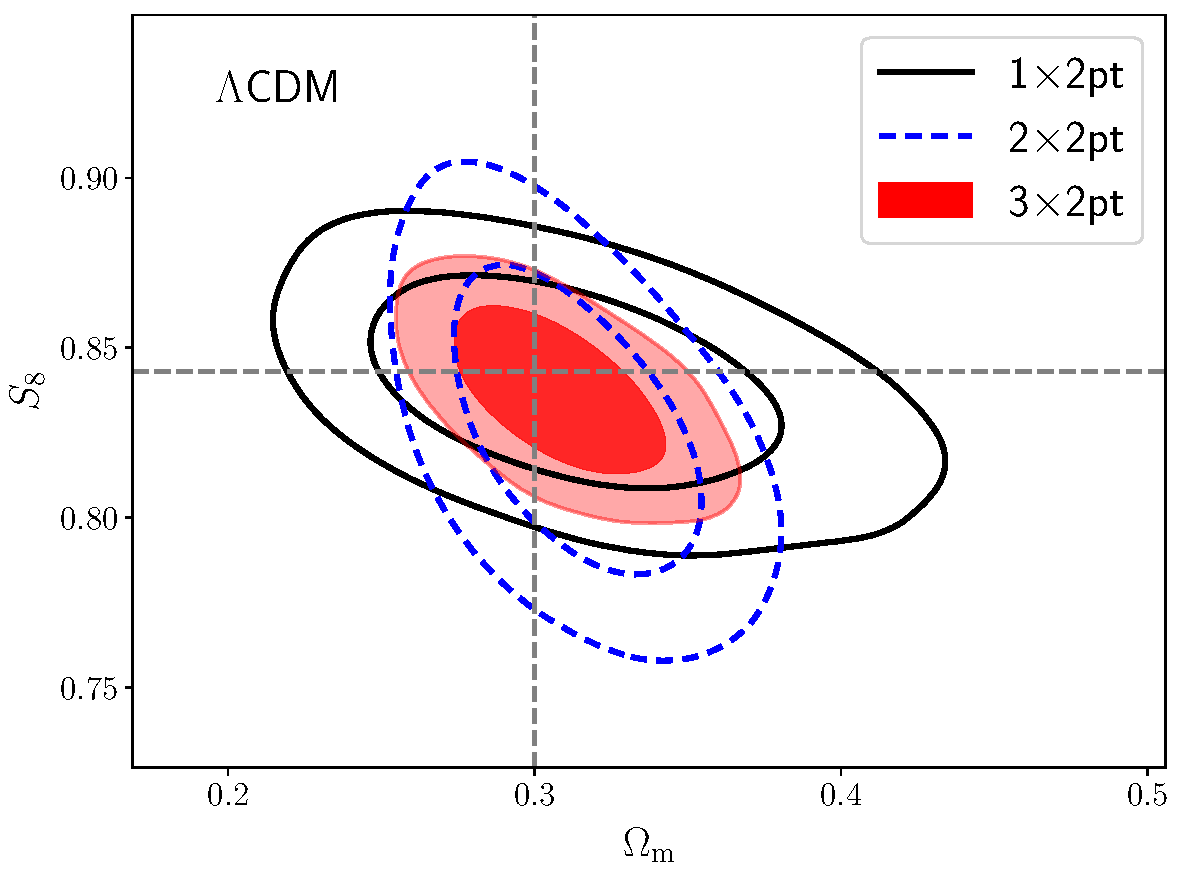
\includegraphics[width=\columnwidth]{figs/simulated_lcdm_compare.pdf}
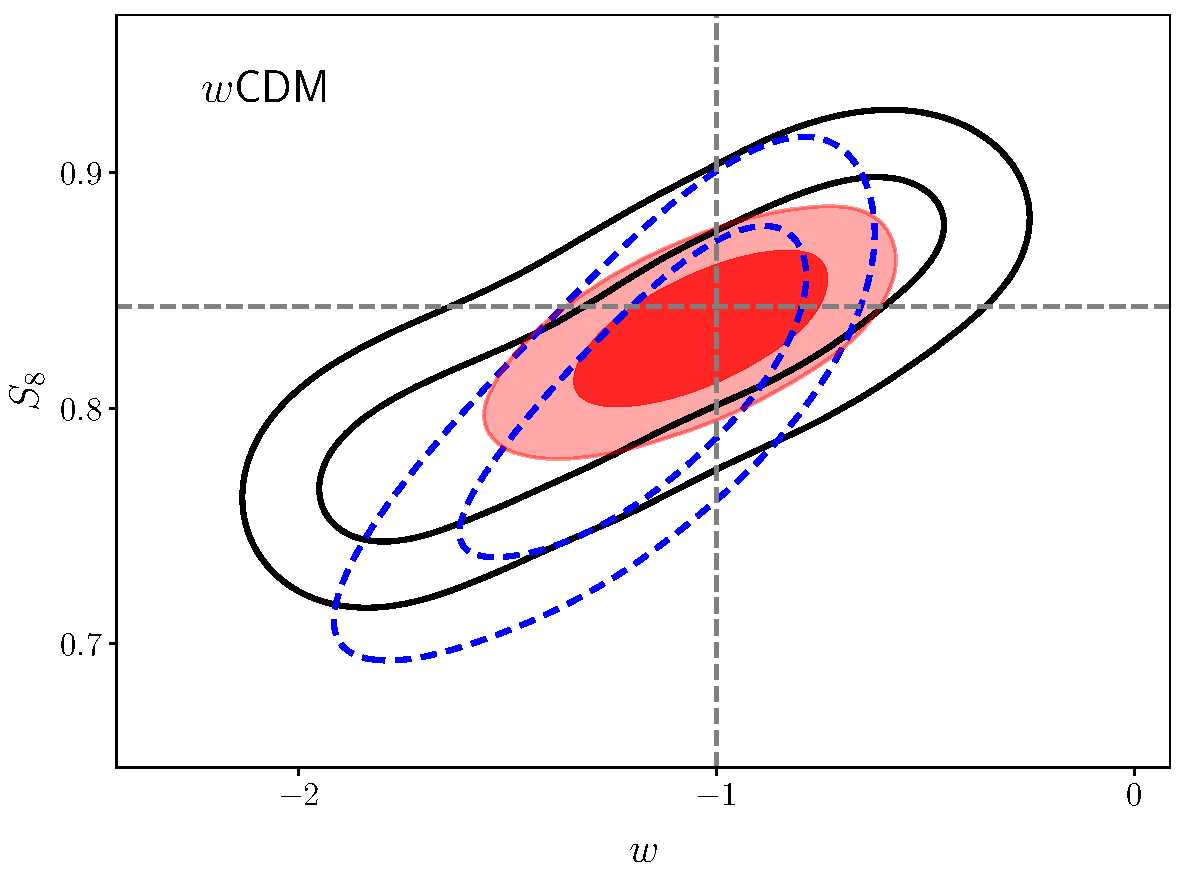
\includegraphics[width=\columnwidth]{figs/simulated_wcdm_compare.pdf}
\caption[]{Comparison of \texit{simulated} constraints on cosmological parameters $\Omega_{\rm m}$ and $S_8$ from cosmic shear alone (1x2pt), galaxy clustering + galaxy-galaxy lensing ($2\times2$pt) and including all three probes ($3\times2$pt). This plot uses a \textit{simulated noise-less baseline datavector} (see \S\ref{sec:simlike_analysis}) and shows that $2\times2$pt adds complementary information to cosmic shear constraints, particularly, providing stronger constraints on $\Omega_{\rm m}$ and $w_0$.}
\label{fig:all2pt_comp}
\end{figure}


\section{Summary Statistics and theory}
\label{sec:stat_theory}
\subsection{Two-point correlations}
Using the catalog of the positions of a lens galaxy sample and the catalog of shapes and positions of weak lensing source galaxies, one can construct three two-point summary statistics: the two-point autocorrelation of the positions of lens galaxies (galaxy clustering), auto-correlation of the lensing shear estimated from the shape of source galaxies (cosmic shear), and cross-correlation of this lensing shear field and position of lens galaxies (galaxy-galaxy lensing). 

In this study, we focus on galaxy clustering and galaxy-galaxy lensing. For galaxy clustering, we use measurements of the $w(\theta)$ statistic, which quantifies the excess number of projected galaxy pairs at a separation $\theta$ over a random distribution. For galaxy-galaxy lensing, we use measurements of the $\gamma_{\rm t}(\theta)$ statistic, which describes the average tangential component of the shear at projected lens-source separation $\theta$. 

We use a hybrid perturbation theory (PT) model to make theoretical predictions for these two-point statistics, as described below. 
% \jdr{make it clear that we use PT and simulations/halo model (halofit is simulation based)}.

\subsubsection{Power spectrum}
\label{sec:Pk_pred}

To compute the two-point projected statistics $\wtheta$ and $\gammat$, we first describe our methodology of predicting galaxy-galaxy and galaxy-matter power spectra ($\pgg$ and $\pgm$ respectively). PT provides a framework to describe the distribution of biased tracers of the underlying dark matter field in quasi-linear and linear scales. This framework allows for an order-by-order controlled expansion of the overdensity of biased tracer (here galaxies) in terms of the overdensity of the dark matter field where successively higher-order non-linearities dominate only in successively smaller scale modes. We will analyze two PT models in this analysis, an effective linear bias model (that is complete only at first order) and an effective one--loop PT model (that is complete up-to third order). 

For the linear bias model, we can write the galaxy-matter cross spectrum as $P_{\mathrm{gm}}(k) = b_1 P_{\mathrm{mm}}$ and auto power spectrum of the galaxies as $P_{\mathrm{gg}}(k) = b_1^2 P_{\mathrm{mm}}(k)$. Here $b_1$ is the linear bias parameter and $P_{\mathrm{mm}}(k)$ is the \emph{non-linear} auto power spectrum of the matter field. 

We use the non-linear matter power spectrum prediction from \citet{Takahashi:2012em} to model (\textsc{Halofit} hereafter) $P_{\mathrm{mm}}(k)$. We use \citet{Bird_halofit} prescription to model the impact of massive neutrinos in this \textsc{Halofit} fitting formula. See \cite{y3-generalmethods} for robustness tests of this choice.  

% \red{We use the halofit as our fiducial choice of matter power spectra. See Methods paper for robustness tests on this choice}
% We discuss our choice of the matter power spectrum in \S\red{matter section}.

In the effective one--loop PT model used here, $P_{\mathrm{gm}}$ and $P_{\mathrm{gg}}$ can be expressed as:
\begin{linenomath*}
\begin{align}\label{eq:P_gg_gm}
    P_{\mathrm{gm}}(k, z) &= b_1 P_{\mathrm{mm}}(k, z) +  \frac{1}{2} b_2 P_{\rm b_1 b_2}(k, z) + \frac{1}{2} b_{\mathrm{s}} P_{\rm b_1 s^2}(k, z) \nonumber  \\
    & + \frac{1}{2} b_{\rm 3nl}P_{\rm b_1 b_{\rm 3nl}}(k, z) \\
    P_{\mathrm{gg}}(k, z) &= b_1^2 P_{\mathrm{mm}}(k, z) + b_1 b_2 P_{\rm b_1 b_2}(k, z) + b_1 b_{\mathrm{s}}P_{\rm b_1 s^2}(k, z) \nonumber \\ 
    & + b_1b_{\rm 3nl} P_{\rm b_1 b_{\rm 3nl} }(k, z) + \frac{1}{4}b_2^2 P_{\rm b_2 b_2}(k, z) + \frac{1}{2} b_2 b_{\mathrm{s}}P_{\rm b_2 s^2}(k, z)  \nonumber \\ 
    & + \frac{1}{4} b^2_{\mathrm{s}} P_{\rm s^2 s^2}(k, z).  
\end{align}
\end{linenomath*}
Here the parameters $ b_1 $, $ b_2 $, $ b_{\mathrm{s}} $ and $ b_{\rm 3nl} $ are the renormalized bias parameters \citep{McDonald2009}. The kernels $P_{\rm b_1 b_2}$, $P_{\rm b_1 s^2}$, $P_{\rm b_1 b_{\rm 3nl}}$, $P_{\rm b_2 b_2}$, $P_{\rm b_2 s^2}$ and $P_{\rm s^2 s^2}$ are described in \cite{Saito2014a}. We validated this model in \cite{p2020perturbation} using 3D correlation functions ($\xigg$ and $\xigm$, which are the Fourier transforms of power spectra mentioned above) of \redmagic galaxies measured in DES-like simulations. We found this model to describe the high signal-to-noise 3D measurements above scales of 4 Mpc/h and redshift $z < 1$ with a reduced $\chi^2$ consistent with one. Our tests also showed that at the projected precision of this analysis, two of the nonlinear bias parameters ($ b_{\mathrm{s}} $ and $ b_{\rm 3nl} $) can be fixed to their co-evolution values given by $b_{\rm s} = (-4/7) (b_1 - 1)$ and $b_{\rm 3nl} = (b_1 - 1)$. We will use this result as our \textit{fiducial} modeling choice of the one--loop PT model. 

% \begin{itemize}
%     \item Heavily referencing the 3D bias paper, describe range of perturbation theory models for $\xigg(r)$ and $\xigm(r)$ and their expected scales of applicability. 
%     \item To aid discussion, include some plots showing the sensitivity of our statistics to scales in $\xigg(r)$ and $\xigm(r)$.
% \end{itemize}

\subsubsection{Angular correlations} \label{sec:proj_2pt}
% \begin{itemize}
%     \item Describe the statistics we use, \wtheta\ and \gammat.
%     \item Show their relation to the underlying 3d correlation functions $\xigg(r)$ and $\xigm(r)$
% \end{itemize}

In order to calculate our observables $\wtheta$ and $\gammat$, we project these 3D power spectra to angular coordinates. %Denoting the normalized redshift distribution of the lens galaxies in tomography bin $i$ by $n^{i}_{\rm g}(z)$ and that of source galaxies in tomography bin $j$ by $n_{\rm s}$, 
The projected galaxy clustering ($AB = \rm{gg}$) and galaxy-galaxy lensing ($AB={\rm g\kappa}$, where $\kappa$ denotes the convergence field) angular power spectra of tomography bins $i,j$ are given by
\begin{linenomath*}
\begin{align}\label{eq:Cl_exact}
    C^{ij}_{AB}(\ell) &= \frac{2}{\pi} \int d\chi_1 W^{\rm i}_{A}(\chi_1) \int d\chi_2 W^{\rm j}_{B}(\chi_2) \nonumber \\
    &\mathrel{\phantom{=}} \int dk \ k^2 \ P_{ AB}(k,z(\chi_1),z(\chi_2)) j_{\ell}(k \chi_1) j_{\ell}(k \chi_2)\,.
\end{align}
\end{linenomath*}
Here $W^{i}_{\rm g}(\chi) = n^{i}_g (z(\chi))dz/d\chi$ is the normalized radial selection function of lens galaxies for tomographic bin $i$ and $W^{\rm i}_{\kappa}$ is the tomographic lensing efficiency of the source sample
\begin{linenomath*}
\begin{equation}
    W^{i}_{\rm \kappa} (\chi)= \frac{3\Omega_{\rm m} H_0^2}{2} \int_{\chi}^{\infty} d\chi' n'_{\rm s} (z(\chi'))\frac{\chi}{a(\chi)}\frac{\chi' - \chi}{\chi'}\,,
\end{equation}
\end{linenomath*}
with $n_{\rm{g/s}}^i(z)$ the normalized redshift distribution of the lens/source galaxies in tomography bin $i$
For the galaxy-galaxy lensing observable, we use the Limber approximation \citep{Limber:53, LoVerde:2008re} which simplifies the above equation to
\begin{linenomath*}
\begin{equation}\label{eq:Cl_limber}
    C^{ij}_{\rm g\kappa}(\ell)  = \int d\chi \frac{W^{i}_{\rm g}(\chi) W^{j}_{\rm \kappa}(\chi)}{\chi^2} P_{\rm g\kappa}\bigg(k=\frac{l + 1/2}{\chi},z(\chi)\bigg)\,.
\end{equation}
\end{linenomath*}
In the absence of other modeling ingredients that are described in the next section, we have $C^{ij}_{\rm g\kappa}(\ell) = C^{ij}_{\rm gm}(\ell)$ (similarly $P_{\rm g\kappa} = P_{\rm gm}$). As described in \citet{Fang_nonlimber}, even at the accuracy beyond this analysis, it is sufficient to use Limber approximation for galaxy-galaxy lensing observable, while for galaxy clustering this may cause significant cosmological parameter biases. 

To evaluate galaxy clustering statistics using Eq.~\ref{eq:Cl_exact}, we split the predictions into small and large scale parts. The non-Limber correction is only significant on large scales where non-linear contributions to the matter power spectra as well as galaxy biasing are sub-dominant. Therefore we use Limber approximation for the small scale non-linear corrections and use non-limber corrections strictly on large scales using linear theory. Schematically, i.e., ignoring contributions from redshift space distorions and lens magnification \cite[c.f.][for details]{y3-generalmethods}, the galaxy clustering angular power spectrum between tomographic bins $i$ and $j$ is given by:
\begin{linenomath*}
\begin{align}\label{eq:Clgg_exact}
    &C_{\rm gg}^{ij} (\ell) \nonumber\\
    &= \int d\chi\, \frac{W_{\rm g}^i(\chi)W_{\rm g}^j(\chi)}{\chi^2} \left[P_{\rm gg}\left(\frac{\ell+0.5}{\chi},\chi\right)- b_1^{i} b_1^{j} P_{\rm lin}\left(\frac{\ell+0.5}{\chi},\chi\right)\right]\nonumber\\
    &+\frac{2}{\pi}\int d\chi_1\,b_{1}^i W_{\rm g}^i(\chi_1) D(z(\chi_1))\int d\chi_2\,b_{1}^j W_{\rm g}^j(\chi_2)D(z(\chi_2))\nonumber\\
    &\;\;\;\;\times \int\frac{dk}{k}k^3 P_{\rm lin}(k,0)j_\ell(k\chi_1)j_\ell(k\chi_2)\,,
\label{eq:Cl-DD_rewrite}
\end{align}
\end{linenomath*}
where $D(z(\chi)$ is the growth factorsand $P_{\rm lin}$ is the linear matter power spectrum. The full model of galaxy clustering including the contributions from other modeling ingredients like redshift space distortions and lens magnification that we describe below is detailed in \cite{Fang_nonlimber} and \cite{y3-generalmethods}. 

The real space projected statistics of our interest can be obtained from these angular correlation via:
\begin{linenomath*}
\begin{align}\label{eq:2pt_exact}
    w^{ij}(\theta) &= \sum \frac{2\ell + 1}{4\pi} \overline{P_{\ell}}(\cos(\theta)) \ C^{ij}_{\rm gg}(\ell) \\
    \gamma_{\rm t}^{ij}(\theta) &= \sum \frac{2\ell + 1}{4\pi \ell (\ell + 1)} \overline{P_{\ell}^2}(\cos(\theta)) \ C^{ij}_{\rm g\kappa}(\ell)
\end{align}
\end{linenomath*}
where $\overline{P_{\ell}}$ and $\overline{P_{\ell}^2}$ are bin-averaged Legendre Polynomials (see \cite{y3-covariances} for exact expressions). 

\subsection{The rest of the model}
\label{sec:model_rest}

% \IR{We need to add more details in a few of the subsections.}
To describe the statistics measured from data, we have to model various other physical phenomena that contribute to the signal to obtain unbiased inferences. In this section, we describe the leading sources of these modeling systematics. We have also validated in \cite{y3-generalmethods} that higher-order corrections do not bias our results. 

\subsubsection{Intrinsic Alignment} 
Galaxy-galaxy lensing aims to isolate the percent-level coherent shape distortions, or shear, of background source galaxies due to the gravitational potential of foreground lens galaxies. However, the local environment, including the gravitational tidal field, can also impact the intrinsic shapes of source galaxies and contribute to the measured shear signal. This interaction between the source galaxies and their local environment, generally known as ``intrinsic alignments'' (IA) is non-random. When there is a non-zero overlap between the source and lens redshift distributions, IA can have a non-zero contribution to the galaxy-galaxy lensing signal. To account for this effect, we model IAs using the ``tidal alignment and tidal torquing'' (TATT) model \citep{Blazek_2019}. Ignoring higher-order effects, such as lens magnification (see \citealp{y3-gglensing}), IA's contribute to the galaxy-shear angular power spectra through the correlation of lens density and the $E$-mode component of intrinsic source shapes: $C^{ij}_{\rm g\kappa}(\ell) \to C^{ij}_{\rm g\kappa}(\ell) + C^{ij}_{\rm gI_{\rm E}}(\ell)$. The $C^{ij}_{\rm gI_{\rm E}}(\ell)$ term is detailed in \cite{y3-generalmethods}, \cite{y3-cosmicshear2}, \cite{y3-gglensing}, and \citet{Blazek_2019}. Within our implementation of the TATT framework, $C^{ij}_{\rm gI_{\rm E}}(\ell)$ for all tomographic bin combinations $i$ and $j$ can be expressed using five IA parameters -- $a_1$ and $a_2$ (normalization of linear and quadratic alignments); $\alpha_1$ and $\alpha_2$ (their respective redshift evolution); and $b_{\rm ta}$ (normalization of a density-weighting term) -- and the linear lens galaxy bias. In principle, there are also contributions at one-loop order in PT involving the non-linear galaxy bias and non-linear IA terms. However, in this analysis, we neglect these terms as we expect them to be subdominant, and they can be largely captured through the free $b_{\rm ta}$ parameter (see \citealp{Blazek_2015} for a further discussion of these terms). 

\subsubsection{Magnification}
All the matter between the observed galaxy and the observer acts as a gravitational lens. Hence, the galaxies get magnified, increasing the size of galaxy images (parameterized by the magnification factor, $\mu$) and increasing their total flux. The increase in the size of galaxies decreases the observed number density (due to stretching of the local sky), whereas increasing the total flux results in an increase in number density (as intrinsically fainter galaxies, which are more numerous, can be observed). This changes the galaxy-galaxy angular power spectrum to: $C^{ij}_{\rm gg}(\ell) \to C^{ij}_{\rm gg}(\ell) + C^{ij}_{\rm \mu g}(\ell) + C^{ij}_{\rm \mu \mu}(\ell) $ and the galaxy-shear angular power spectrum to $C^{ij}_{\rm g\kappa}(\ell) \to C^{ij}_{\rm g\kappa}(\ell) + C^{ij}_{\rm \mu I_{\rm E}}(\ell) + C^{ij}_{\rm \mu \kappa}(\ell)$. The auto and cross-power spectra with magnification are again given by Eq.\ref{eq:Cl_exact}. See \cite{y3-generalmethods} for the detailed description of the equations for each of the power spectra. 

The magnification coefficients are computed with the Balrog image simulations \citep{Suchyta_2016,y3-balrog} in a process described in \cite{y3-2x2ptmagnification}. We refer the reader to \citet{y3-2x2ptmagnification} for further details about the impact of magnification on our observable and their constraints from data. Galaxy profiles are drawn from the DES deep fields \cite{deepfields} and injected into real DES images. The full photometry pipeline \cite{Y3Gold} and \redmagic\ sample selection is applied to the new images to produce a simulated \redmagic\ sample with the same selection effects as the real data. To compute the impact of magnification, the process is repeated, this time applying a constant magnification to each injected galaxy. The magnification coefficients are then derived from the fractional increase in number density when magnification is applied. This method captures both the impact of magnification on the galaxy magnitudes and the galaxy sizes, including all numerous sample selection effects. 

\subsubsection{Non-locality of galaxy-galaxy lensing}  \label{sec:pm_theory}
The configuration space estimate of the galaxy-galaxy lensing signal is a
non-local statistic even on linear scales. The galaxy-galaxy lensing
signal of source galaxy at redshift ($z_{\rm s}$) by the matter around
galaxy at redshift $z_{\rm l}$ at perpendicular to the line of sight
distance $R$ is related to the mass density of matter around lens
galaxy by:
\begin{linenomath*}
\begin{equation}
    \gamma_{\rm t}(R;z_{\rm g},z_{\rm s}) = \frac{\Delta \Sigma (R;z_{\rm l})}{\Sigma_{\rm crit} (z_{\rm g},z_{\rm s})},
\end{equation}
\end{linenomath*}
where, $\Delta \Sigma(R;z_{\rm l}) = \bar{\Sigma}(0,R; z_{\rm l}) - \Sigma(R;z_{\rm l})$ and $\Sigma(R;z_{\rm l})$ is the surface mass density at a transverse separation $R$ from the lens and $\bar{\Sigma}(0,R)$ is the average surface mass density within a separation $R$ from that lens. Through the $\bar{\Sigma}(0,R)$ term, $\gamma_{\rm t}$  at any scale $R$, is dependent on the mass distribution at all scales less than $R$. This makes $\gamma_{\rm t}$  highly non-local and any model that is valid only on large scales above some $r_{\rm min}$ (like PT) will break down more rapidly than for a more local statistic like \wtheta. However, as the dependence on small scales is through the \textit{mean} surface mass density, the impact of mass distribution inside $r_{\rm min}$ on $\gammat$ can be written as:
\begin{linenomath*}
\begin{equation}
    \gamma_{\rm t}(R;z_{\rm g},z_{\rm s}) = \frac{1}{\Sigma_{\rm crit}(z_{\rm g},z_{\rm s})} \bigg(\Delta \Sigma_{\rm model}(z_{\rm g}) + \frac{B(z_{\rm g})}{R^2} \bigg),
\end{equation}
\end{linenomath*}
where, $\Delta \Sigma^{\rm model}$ is the prediction from a model (which in here is given by PT) that is valid on scales above $r_{\rm min}$. Here, $B$ is the effective total residual mass below $r_{\rm min}$ and is known as point mass (PM) parameter. In this analysis we use the thin redshift bin approximation (see Appendix~\ref{app:pm} for details of this validation) and hence the average $\gamma_{\rm t}$ signal between lens bin $i$ and source bin $j$ can be written as:
\begin{linenomath*}
\begin{equation}
    \gamma^{ij}_{{\rm t}} = \gamma^{ij}_{{\rm t, model}} + G^{ij}/\theta^2,
\end{equation}
\end{linenomath*}
where,

\begin{linenomath*}
\begin{equation}\label{eq:pm_Cij}
    G^{ij} = B^i \, \int dz_{\rm g} \ dz_{\rm s} \ n^{i}_{{\rm g}} \ n^{j}_{{\rm s}} \ \Sigma^{-1}_{\rm crit}(z_{\rm g},z_{\rm s}) \ \chi^{-2}(z_{\rm g}) \equiv B^i \, \beta^{ij}
\end{equation}
\end{linenomath*}
Here $B^i$ is the PM for lens bin $i$, $n^{i}_{{\rm g}}$ is the redshift distribution of lens galaxies for tomographic bin $i$, $n^{j}_{{\rm s}}$ is the redshift distribution of source galaxies for tomographic bin $j$. 
% Note that this approximation also retains the shear ratio information in our analysis. 

However, instead of directly sampling over the parameters $B^i$ for each tomographic bin, we implement an analytic marginalization scheme as described in \cite{MacCrann:2019ntb}. We modify our inverse-covariance when calculating the likelihood as described in \S\ref{sec:cov_pm}

    

\section{Data description}

\subsection{DES Y3}

The full DES survey was completed in 2019 using the Cerro Tololo Inter-American Observatory (CTIO) 4 m Blanco telescope in Chile and covered approximately 5000 square degrees of the South Galactic Cap. This 570- megapixel Dark Energy Camera \citep{Flaugher15} images the field in five broadband filters, \textit{grizY}, which span the wavelength range from approximately 400nm to 1060nm. The raw images are processed by the DES Data Management team \citep{Sevilla11, Morganson18} and after a detailed object selection criteria on the first three years of imaging data (detailed in \citet{Abbott_2018}) Y3 \gold data set containing 400 million sources are constructed.  (data without additional metadata is available as Data Release 1\footnote{https://des.ncsa.illinois.edu/releases/dr1} ). We further process this \gold data set to obtain the lens and source catalogs described in the following sub-sections.


\subsubsection{\redmagic lens galaxy sample}

The principal lens sample used in this analysis is selected with the \redmagic algorithm \citep{Rozo_2016} run on DES Year 3 data. \redmagic selects Luminous Red Galaxies (LRGs) according to the magnitude-color-redshift relation of red sequence galaxies, calibrated using an overlapping spectroscopic sample.
% from \blue{<SPEC Z SAMPLE, OZDES? ask Eli>}. 
This sample has a threshold luminosity $L_{\rm min}$ and constant co-moving density. The full \redmagic algorithm is described in \citet{Rozo_2016}, and after application of this algorithm to DES Y3 data, we have approximately 2.6 million galaxies.

% \blue{Mention about high-density and high luminosity differences}

In \cite{y3-galaxyclustering} it was found the \redmagic number density fluctuates with several observational properties of the survey, which imprints a non-cosmological bias into the galaxy clustering. To account for this we assign a weight to each galaxy, which corresponds to the inverse of the angular selection function at that galaxies location. The computation and validation of these weights is described in \cite{y3-galaxyclustering}.  


\subsubsection{\maglim lens galaxy sample}
We also compare and show the constraints using an alternative lens sample selected by implementing a redshift-dependent magnitude cut on the $i$-band magnitude of the \gold catalog. We denote this sample by \maglim, which is detailed in \citet{y3-2x2ptaltlensresults}.


\subsubsection{Source galaxy shape catalog}

To estimate the weak lensing shear of the observed source galaxies, we use the \metacal algorithm. This method estimates the response of a shear estimator to artificially sheared galaxy images and incorporates improvements like better PSF estimate \citep{y3-piff}, better astrometric methods \citep{y3-gold} and inclusion of inverse variance weighting. The details of the method applied to our galaxy sample are presented in \cite{y3-shapecatalog}. This methodology does not capture the object blending effects and shear-dependent detection biases and we use image simulations to calibrate this bias as detailed in \citet{y3-imagesims}. The galaxies that pass the selection cuts designed to reduce systematic biases (as detailed in \citet{y3-shapecatalog}) are used to make our source sample shape catalog. This catalog consists of approximately 100 million galaxies with effective number density of $n_{\rm eff} = 5.6$ galaxies per ${\rm arcmin}^2$ and an effective shape noise of $\sigma_{\rm e} = 0.26$.


% \subsubsection{Photoz calibration}

\subsection{$\buzzard$ Simulations}

% \subsubsection{$\buzzard$ sims}
The \buzzard\ simulations are $N$-body lightcone simulations that have been populated with galaxies using the \textsc{Addgals} algorithm \citep{Addgals}, endowing each galaxy with positions, velocities, spectral energy distributions, broad band photometry, half-light radii and ellipticities. Each pair of 2 Y3 simulations are produced from a set of 3 independent $N$-body lightcones with box sizes of $1.05,\, 2.6 \textrm{ and } 4.0\, (h^{-3}\, \rm Gpc^3)$, mass resolutions of $3.3\times10^{10},\, 1.6\times10^{11},\, 5.9\times10^{11}\, h^{-1}M_{\odot}$, spanning redshift ranges $0.0< z \leq 0.32$, $0.32< z \leq 0.84$ and $0.84< z \leq 2.35$ respectively. Together these produce $10,000$ square degrees of unique lightcone. The lightcones are run with the \textsc{L-Gadget2} $N$-body code, a memory optimized version of \textsc{Gadget2} \citet{Springel_2005}, with initial conditions generated using \textsc{2LPTIC} at $z=50$ \citep{Crocce2012}. 

The \textsc{Addgals} model uses the relationship, $P(\delta_{R}|M_r)$, between a local density proxy, $\delta_{R}$, and absolute magnitude $M_r$ measured from a high-resolution subhalo abundance matching (SHAM) model in order to populate galaxies into these lightcone simulations. This model reproduces the absolute--magnitude--dependent clustering of the SHAM. Additionally, we employ a conditional abundance matching (CAM) model, assigning redder SEDs to galaxies that are closer to massive dark matter halo, in a manner that allows us to reproduce the color-dependent clustering measured in the Sloan Digital Sky Survey Main Galaxy Sample (SDSS MGS) \citep{Addgals, DeRose2020b}. 

These simulations are ray-traced using the spherical-harmonic transform (SHT) configuration of \textsc{Calclens}, where the SHTs are performed on an $N_{\rm side}=8192$ \textsc{HealPix} grid \citep{Becker2013}. The lensing distortion tensor is computed at each galaxy position and is used to deflect the galaxy angular positions, shear galaxy intrinsic ellipticities, including effects of reduced shear, and magnify galaxy shapes and photometry. We have conducted convergence tests of this algorithm and found that resolution effects are negligible on the scales used for this analysis \citep{DeRose2019}.

Once the simulations have been ray-traced, we apply DES Y3 specific masking and photometric errors. To mask the simulations, we employ the Y3 footprint mask but do not apply the bad region mask \citep{y3-gold}, resulting in a footprint with an area of 4143.17 square degrees. Each set of 3 $N$-body simulations yields 2 Y3 footprints that contain 520 square degrees of overlap.

We apply a photometric error model to simulate wide-field photometric errors in our simulations. To select a lens galaxy sample, we run the \redmagic\ galaxy selection on our simulations using the same configuration as used in the Y3 data, as described in \citet{y3-galaxyclustering}. A weak lensing source selection is applied to the simulations using PSF-convolved sizes and $i$-band SNR to match the non-tomographic source number density, 5.9 $arcmin^{-2}$, in the \metacal\ source catalog. We employ the SOMPZ redshift estimation framework to our simulations in order to place galaxies into four source redshift bins with number densities of 1.46 $\rm arcmin^{-2}$ each. Once binned, we match the shape noise of the simulations to that measured in the \metacal\ catalog per tomographic bin, yielding shape noise values of $\sigma_{e}=[0.247, 0.266, 0.263, 0.314]$.

Two-point functions are measured in the \buzzard\ simulations using the same pipeline used for the DES Y3 data, where we set \metacal\ responses and inverse variance weights equal to 1 for all galaxies, as these are not assigned in our simulation framework. Lens galaxy weights are produced in a manner similar to that done in the data and applied to measure our clustering and lensing signals. The clustering and galaxy-galaxy lensing predictions match the DES \redmagic\ measurements to $10-20\%$ accuracy over most scales and tomographic bins, except for the first lens bin, which disagrees by $50\%$ in \wtheta\. See \citet{y3-simvalidation} for a more detailed comparison.

\subsection{Datavector}

\subsubsection{\redmagic redshift methodology}
\label{sec:lensz}
We split the \redmagic sample into $N_{\rm z,g} = 5$ tomographic bins, selected on the \redmagic redshift point estimate quantity ZREDMAGIC. The bin edges used are $z=0.15, 0.35, 0.50, 0.65, 0.80, 0.90$. The first three bins use a luminosity threshold of $L_{\min} > 0.5 L_{*}$ and are known as the high-density sample. The last two redshift bins use a luminosity threshold of $L_{\min} > 1.0 L_{*}$ and are known as the high luminosity sample.

The redshift distributions are computed by stacking four samples from the PDF of each \redmagic galaxy, allowing for the non-gaussianity of the PDF. We find an average individual redshift uncertainty of $\sigma_z/(1+z) < 0.0126$ in the redshift range used from the variance of these samples.

\subsubsection{\maglim redshift methodology}

\subsubsection{Source redshift methodology}
\label{sec:sourcez}
The methodology for calibrating the photometric redshifts of the distribution of our source galaxies is summarized in \citet{y3-sompz}. Overall, the redshift calibration methodology involves the use of self-organizing maps \citep{y3-sompz}, clustering redshifts \citep{y3-sourcewz} and shear-ratio \citep{y3-shearratio} information. The self-organizing map methodology uses DES deep-field observations \citep{y3-deepfields} as a training dataset and provides redshift distribution samples after including the uncertainties from sample variance and galaxy flux measurements. The clustering redshifts methodology uses the calibration using \redmagic and BOSS/eBOSS dataset and filters out the less likely redshift distribution samples. These two approaches provide us the mean redshift distribution of source galaxies and uncertainty in this distribution. The shear-ratio calibration uses the ratios of small scales galaxy-galaxy lensing data, which is largely independent of the cosmological but helps calibrate the uncertainties in the redshift distributions. We include as an external likelihood in our analysis, as briefly described in \S\ref{sec:shear_ratio} and detailed in \citet{y3-shearratio}. 

Finally, we split source catalog into $N_{\rm z,s} = 4$ tomographic bins.The mean redshift distribution of lenses and sources are compared in the Fig.~\ref{fig:nz_comp}.
\begin{figure}
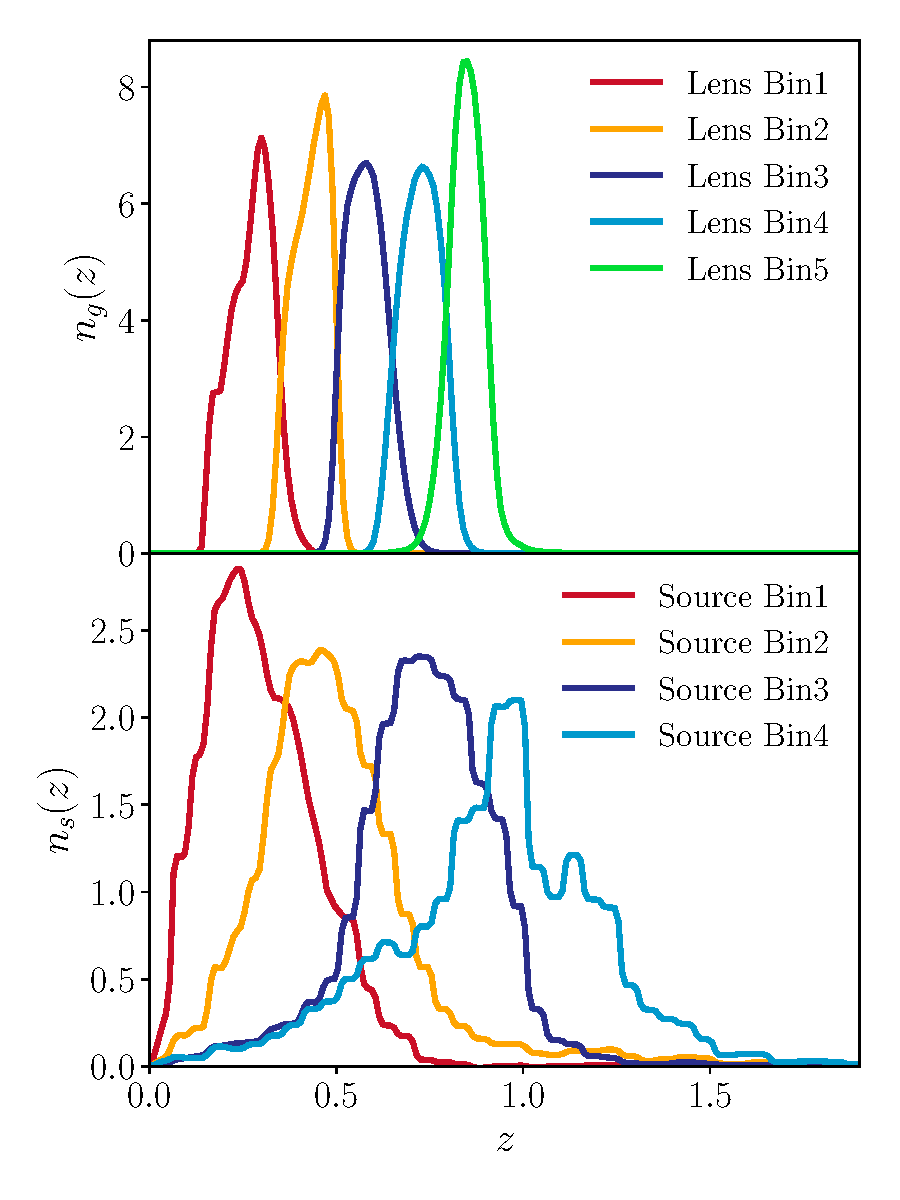
\includegraphics[width=0.48\textwidth]{figs/nz_DES.pdf}
\caption[]{Comparison of the normalized redshift distribution of source galaxies and \redmagic lens galaxies in the data.}
\label{fig:nz_comp}
\end{figure}

\subsubsection{2pt measurements}\label{sec:2pt_data}
% \blue{Describe the 2pt measurements for both $\wtheta$ and $\gammat$. Mention the combined SNR of these measurements. Mention that we do the measurements in the 20 radial bins for any two tomographic bin combinations. Mention that for $\wtheta$ we only use auto-bins. Introduce $N_{\rm data}$ and how it relates to the number of elements for $\wtheta$ and the number of $\gammat$ elements.} 

For galaxy clustering, we use the Landy-Szalay estimator given as:
\begin{linenomath*}
\begin{equation}
    w(\theta) = \frac{DD - 2DR + RR}{RR}
\end{equation}
\end{linenomath*}
where $DD$, $DR$ and $RR$ are normalized weighted number counts of galaxy-galaxy, galaxy-random and random-random pairs within angular and tomographic bins. For lens tomographic bin, we measure the auto-correlations in $N_{\theta} = 20$ log-spaced angular bins ranging from 2.5arcmin to 250arcmin. Each lens galaxy in the catalog ($g_i$) is weighted with its systematic weight $w_{\rm g_i}$. This systematic weight aims to remove the correlations between the large scale fluctuations due to changing observing conditions in the telescope and the cosmological density field. Our randoms catalog is 40 times larger than the galaxy catalog. The validation of this estimator and systematic weights of the lens galaxies is presented in \cite{y3-galaxyclustering}. In total we have $N_{\wtheta} = N_{\rm z,g} \times N_{\theta} = 100$ measured $\wtheta$ datapoints. 


The galaxy-galaxy lensing estimator including the effects of boost factors, random point subtraction and shear responses is given by:
\begin{linenomath*}
\begin{equation}
    \gamma_{\rm t}(\theta) = \frac{\sum_k w_{\textrm{r}_k}}{\sum_i w_{\textrm{g}_i}} \frac{\sum_{ij} w_{\textrm{g}_i} w_{\textrm{s}_j} e^{\rm LS}_{{\rm t},ij}}{\sum_{kj} w_{\textrm{r}_k} w_{\textrm{s}_j}} - \frac{\sum_{kj} w_{\textrm{r}_k} w_{\textrm{s}_j} e^{\rm RS}_{{\rm t},kj}}{\sum_{kj} w_{\textrm{r}_k} w_{\textrm{s}_j}}
\end{equation}
\end{linenomath*}
where $e^{\rm LS}_{{\rm t},ij}$ and $e^{\rm RS}_{{\rm t},kj}$ is the measured tangential ellipticity of source galaxy $j$ around lens galaxy $i$ and random point $k$ respectively. The weights $w_{\textrm{g}_i}$ is the systematic weight of lens galaxy as described above, $w_{\textrm{r}_k}$ is the weight of random point that we fix to 1 and $w_{\textrm{s}_j}$ is the weight of the source galaxy that is computed from inverse variance of the shear response weighted ellipticity of the galaxy (see \cite{y3-shapecatalog} for details). This estimator has been detailed and validated in \cite{y3-gglensing}. We measure this signal for each pair of lens and source tomographic bins and hence in total we have  $N_{\gammat} = N_{\rm z,g} \times N_{\rm z,s} \times N_{\theta} = 400$ measured $\gammat$ datapoints. 

We analyze both of these measured statistics jointly and hence we have in total $N_{\rm data} = N_{\wtheta} + N_{\gammat} = 500$ datapoints. Our measured signal to noise of $\wtheta$ is 177$\sigma$ \citep{y3-galaxyclustering}, of  $\gammat$ is 121$\sigma$ \citep{y3-gglensing}; giving total joint total signal to noise of 201$\sigma$. 

\subsubsection{Shear ratios}\label{sec:shear_ratio}
As will be detailed in \S\ref{sec:scale_cuts}, in this analysis, we remove the small scales' non-linear information from the 2pt measurements that are presented in the above sub-section. However, as presented in \citet{y3-shearratio}, the ratio of $\gammat$ measurements for the same lens bin but different source bins is well described by our model (see \S\ref{sec:stat_theory}) even in small scales. Therefore we include these ratios (referred to as shear-ratio henceforth) as an additional independent dataset in our likelihood. In this shear-ratio datavector, we use the angular scales above the scale cuts of 2Mpc/$h$ and less than our fiducial scale cuts for 2pt measurements described in \S\ref{sec:scale_cuts} (we also leave two datapoints between 2pt scale cuts and shear-ratio scale cuts to remove any potential correlations between the two). The details of the analysis choices for shear ratios measurements and its covariance are detailed in \citet{y3-shearratio} and \citet{y3-3x2ptkp}. 

% \SP{A short paragraph about blinding and tests that we passed before unblinding}

% \subsubsection{Blinding}

% \subsubsection{Unblinding}


\subsection{Covariance}
\label{sec:cov}

In this analysis, the covariance between the statistic $\wtheta$ and $\gammat$ (${\mathbfcal{C}}$) is modeled as sum of gaussian term ($\mathbfcal{C}_{\rm G}$), trispectrum term ($\mathbfcal{C}_{\rm NG}$) and super-sample covariance term ($\mathbfcal{C}_{\rm SSC}$). The analytic model used to describe ($\mathbfcal{C}_{\rm G}$) is described in \cite{y3-covariances}. The terms $\mathbfcal{C}_{\rm NG}$ and $\mathbfcal{C}_{\rm SSC}$ are modeled using a halo model framework as detailed in \cite{Krause:2016jvl, Krause2017}. The covariance calculation has been performed using CosmoCov package \citep{Fang:2020vhc} package and the robustness of this covariance matrix has been tested and detailed in \cite{y3-covariances}. 

\subsubsection{Point mass analytic marginalization}
\label{sec:cov_pm}
As mentioned in \S~\ref{sec:pm_theory}, we modify the inverse-covariance to perform analytic marginalization over the PM parameters. As detailed in \cite{MacCrann:2019ntb}, using generalization of Sherman-Morrison formula, this procedure changes our fiducial inverse-covariance ${\mathbfcal{C}}^{-1}$ to ${\mathbfcal{C}}^{-1}_{\rm wPM}$ as follows:
\begin{linenomath*}
\begin{equation}
    {\mathbfcal{C}}^{-1}_{\rm wPM} = {\mathbfcal{C}}^{-1} - {\mathbfcal{C}}^{-1} {\mathbfcal{U}} ({\mathbfcal{I}} + {\mathbfcal{U}}^{\rm T} {\mathbfcal{C}}^{-1} {\mathbfcal{U}})^{-1} {\mathbfcal{U}}^{\rm T} {\mathbfcal{C}}^{-1}
\end{equation}
\end{linenomath*}

Here ${\mathbfcal{C}}^{-1}$ is the inverse of the halo-model covariance as described above, $\mathbfcal{I}$ is the unity matrix and $\mathbfcal{U}$ is a $N_{\rm data} \times N_{\rm z,g}$ matrix where $i$-th column is given by $\sigma_{B^i} \vec{t}^{i}$. Here $\sigma_{B^i}$ is the standard deviation of gaussian prior on point mass parameter $B^i$ and $\vec{t}^{i}$ is given as:
\begin{linenomath*}
\begin{equation}
    \bigg(\vec{t}^{i} \bigg)_{a} = \begin{cases}
0 & \parbox{5cm}{if $a$-th element is not corresponding to $\gammat$ and if lens-redshift of $a$-th element $\neq i$} \\  
\\
\beta^{ij}\theta_{a}^{-2} &\text{otherwise}
\end{cases}
\end{equation}
\end{linenomath*}
where the expression for $\beta^{ij}$ is shown in Eq.\ref{eq:pm_Cij}. We evaluate that term at fixed \textit{fiducial} cosmology as given in Table \ref{tab:params_all}. In our analysis we put a wide prior on PM parameters $B^i$ by choosing $\sigma_{B^i} = 10000$ which translates to effective mass residual prior of $10^{17} M_{\odot}/h$ (see Eq.~\ref{eq:pm_halo})



\section{Validation of parameter inference}

We assume the likelihood to be a multivariate Gaussian
\begin{linenomath*}
\begin{equation}
    \ln \mathcal{L}(\vec{\mathbfcal{D}}|\Theta) = -\frac{1}{2} (\vec{\mathbfcal{D}} - \vec{\mathbfcal{T}}(\Theta)) \, {\mathbfcal{C}}^{-1}_{\rm wPM} \,  (\vec{\mathbfcal{D}} - \vec{\mathbfcal{T}}(\Theta))^{\rm T}
\end{equation}
\end{linenomath*}
Here $\vec{\mathbfcal{D}}$ is the measured $\gammat$ and $\wtheta$ datavector of length $N_{\rm data}$ (if we use all the angular and tomograhic bins), $\vec{\mathbfcal{T}}$ is the theoretical prediction for these statistics for the parameter values given by  $\Theta$, and ${\mathbfcal{C}}^{-1}_{\rm wPM}$ is the inverse covariance matrix of shape $N_{\rm data} \times N_{\rm data}$ (including modifications from the PM marginalization term).

For our analysis we use the \textsc{Polychord} sampler with the settings described in \cite{y3-samplers}. The samplers probe the posterior volume ($\mathcal{P}(\Theta | \vec{\mathbfcal{D}})$) which is given by:
\begin{linenomath*}
\begin{equation}
    \mathcal{P}(\Theta | \vec{\mathbfcal{D}}) = \frac{\mathcal{L}(\vec{\mathbfcal{D}}|\Theta) {\rm P}(\Theta)}{{\rm P}(\vec{\mathbfcal{D}})}
\end{equation}
\end{linenomath*}
where ${\rm P}(\Theta)$ are the priors on the parameters of our model, described in \S\ref{sec:prior}, and ${\rm P}(\vec{\mathbfcal{D}})$ is the evidence of data. 

To estimate the constraints on the cosmological parameters, we have to marginalize the posterior over all the rest of the multi-dimensional parameter space. We quote the mean and 1$\sigma$ variance of the marginalized posteriors when quoting the constraints. However, note that these marginalized constraints can be biased if the posterior has significant non-gaussianities due to projection effects. The maximum-a-posteriori (MAP) point is not affected by the projection effects; therefore, we also show this in our plots. However, we note that in high-dimensional parameter space with a non-trivial structure, it is difficult to converge on a global maximum of whole posterior as we have here.


\subsection{Analysis choices}
\label{sec:analysis_choices}
In this subsection, we detail the galaxy bias models that we use, describe the free parameters of our models, and choose priors on those parameters. 
\subsubsection{PT Models}
\label{sec:pt_models}
In this analysis, we test two different galaxy bias models:
\begin{enumerate}
    \item \textit{Linear bias} model: The simplest model to describe the overdensity of galaxies, valid at large scales, assumes it to be linearly biased with respect to the dark matter overdensity (see \S~\ref{sec:Pk_pred}). In this model, for each lens tomographic bin $j$, the average bias of galaxies is given by a constant free parameter $b^j_1$. 
    \item \textit{Non-linear bias} model: 
    To describe the clustering of galaxies at smaller scales robustly, we also implement a one--loop PT model. As described in the \S~\ref{sec:Pk_pred}, in general, this model has four free bias parameters for each lens tomographic bin. For each tomographic bin $j$, we fix three of the non-linear parameters to their co-evolution value given by: $b^{j}_{\rm s} = (-4/7) (b^j_1 - 1)$ and $b^{j}_{\rm 3nl} = b^j_1 - 1$ \citep{McDonald2009,Saito2014a}. Therefore, in our implementation, we have two free parameters for each tomographic bin: linear bias $b^{j}_1$ and non-linear bias $b^{j}_2$. This allows us to probe smaller scales with minimal extra degrees of freedom, obtaining tighter constraints on the cosmological parameters while keeping the biases due to projection effects, as described below, in control. 
    % \jdr{Probably good to emphasize that this choice is largely driven by our desire to minimize projection effects. If we could, we would want to marginalize over all of these parameters}.
    
    As we describe below, in order to test the robustness of our model, we analyze the bias in the marginalized constraints on cosmological parameters. However, given asymmetric non-Gaussian degeneracies between the parameters of the model (particularly between cosmological parameters and poorly constrained non-linear bias parameters $b^{j}_2$ and intrinsic alignment parameters), the marginalized constraints show projection effects. We find that sampling the non-linear bias model parameters in combination with $\sigma_8$, as $b^{j}_1 \sigma_8$ and $b^{j}_2 \sigma^2_8$ removes much of the posterior projection effect. As detailed later, these parameters are sampled with flat priors. We emphasize that the flat priors imposed on these non-linear combinations of parameters are non-informative and our final constraints on $b^{j}_1$ and $b^{j}_2$ are significantly tighter than the projection of priors on these parameters.
    % \red{In the end, we care about the posterior on the cosmology parameters. This requires marginalizing over all the free parameters of the model. $\wtheta$ and $\gammat$ has a lower signal to noise and hence can not constrain the higher-order parameters like $b^j_2$ tightly. When projecting this to lower dimension space, the posterior-mass due to non-linear parameters being far from the truth can bias the constraints on the marginalized parameters due to subtle degeneracies. This is known as projection effect or volume effect.} We find that using a uniform prior on the linear and non-linear bias parameters lead to large projection effects.  Therefore, we choose to sample the parameters $b^{j}_1 \sigma_8$ and $b^{j}_2 \sigma^2_8$ which helps in removing much of the projection effect. \red{This choice is motivated because the overdensity of galaxy is approximately given by $\delta_g \sim b_1 \delta_m + b_2 \delta_m^2$.} We use wide uninformative uniform priors on these parameters for each tomographic bin $j$ given by : $0.67 < b^{j}_1 \sigma_8 < 3.0$ and $-4.2 < b^{j}_2 \sigma^2_8 < 4.2$. At each point in the parameter space, we calculate the $\sigma_8$ and retrieve the bias parameters $b^{j}_1$ and $b^{j}_2$ from the sampled parameters $b^{j}_1$ and $b^{j}_2$.
\end{enumerate}


\subsubsection{Cosmological Models}
\label{sec:cosmo_models}
% \subsection{Cosmological models, external datasets and priors}
% We test the following cosmological models in this work:
We report the constraints on two choices of the cosmological model:
\begin{enumerate}
    \item Flat \lcdm\ with uninformative priors: We free six cosmological parameters $\Omega_{\rm m}$, $\Omega_{\rm b}$, $n_{\rm s}$, $h_0$, $A_s$ and $\Omega_\nu h^2$.
    \item Flat \wcdm : In addition the six parameters listed above, we also free $w_0$.
\end{enumerate}


\subsubsection{Scale cuts}\label{sec:scale_cuts}

The complex astrophysics of galaxy formation, evolution, and baryonic processes like feedback from active galactic nuclei (AGN), supernovae explosions, and cooling make higher-order non-linear contributions that we do not include in our model. The contribution from these poorly understood effects can exceed our statistical uncertainty on the smallest scales; hence we apply scale cuts chosen so that our PT models give unbiased cosmological constraints.% when analyzing a datavector that receives a contribution from higher-order non-linearities at a level that we expect to be present in our measurements. 

As mentioned earlier, marginalizing over a multi-dimensional parameter space can lead to biased 2D parameter constraints due to projection effects. To calibrate this effect for each of our models, we first perform an analysis using a \textit{baseline} datavector constructed from \textit{fiducial} values of that model. 
%Due to projection effects, we do not expect the marginalized contours of this \textit{baseline} analysis to be centered at the true cosmology, and the difference between them is a measure of the expected projection effect. 
We then run our MCMC chain on the \textit{contaminated} datavector that includes higher-order non-linearities, and we measure the bias between the peak of the marginalized \textit{baseline} contours and the peak of the marginalized \textit{contaminated} contours. 

From the tests on 3D correlation functions at fixed cosmology in simulations \citep{p2020perturbation}, we find that the \textit{linear bias} model is a good description above 8Mpc/$h$ while the two-parameter \textit{non-linear bias} model describes the correlations above 4Mpc/$h$. We convert these physical co-moving distances to angular scale cuts for each tomographic bin and treat them as starting guesses. Then for each model, we iterate over scale cuts until we find the minimum scales at which the bias between marginalized \textit{baseline} and \textit{contaminated} contours is less than $0.3\sigma$. For \lcdm\ model, we impose this criterion on the $\Omega_{\rm m}-S_8$ projected plane, and for $w$CDM model, we impose this criterion on all three 2D plane combinations constructed out of $\Omega_{\rm m}$, $S_8$ and $w$. Further validation of these cuts is performed using simulations in \ref{sec:sims} and \citet{y3-simvalidation}. 



\subsubsection{Priors and Fiducial values}
\label{sec:prior}
We use non-informative priors on the cosmological parameters to ensure statistically independent constraints on them. Although our constraints on cosmological parameters like the Hubble constant $h$, spectral index $n_{\rm s}$ and baryon fraction $\Omega_{\rm b}$ are modest compared to surveys like \textit{Planck}, we have verified that our choice of wide priors does not bias the inference on our cosmological parameters of interest, $\Omega_{\rm m}$ and $S_8$. 

When analyzing the \textit{linear bias} model, we use a wide uniform prior on these linear bias parameters, given by $0.5 < b^{j}_1 < 3$. For the \textit{non-linear bias} model, as mentioned above, we sample the parameters $b^{j}_1 \sigma_8$ and $b^{j}_2 \sigma^2_8$. We use uninformative uniform priors on these parameters for each tomographic bin $j$ given by $0.67 < b^{j}_1 \sigma_8 < 3.0$ and $-4.2 < b^{j}_2 \sigma^2_8 < 4.2$. At each point in the parameter space, we calculate  $\sigma_8$ and retrieve the bias parameters $b^{j}_1$ and $b^{j}_2$ from the sampled parameters to get the prediction from the theory model. The fiducial values of the linear bias parameters $b^{j}_1$ used in our simulated likelihood tests are motivated by the  recovered bias values in N-body simulations and are summarized in Table \ref{tab:params_all}. 
For the non-linear bias parameters, the fiducial value of $b^{j}_2$ are obtained from the interpolated $b_1-b_2$ relation extracted from 3D tests in \mice simulations (see Fig.8 of \cite{p2020perturbation}) for fiducial $b^j_1$ for each tomographic bin.

For the intrinsic alignment parameters, we again choose uniform and uninformative priors. As the IA parameters are directly dependent on the source galaxy population, it is challenging to motivate a reasonable choice of prior from other studies. The fiducial values of these parameters required for the simulated test are motivated by the Y1 analysis as detailed in \cite{Samuroff_2019}.

We impose an informative prior for our measurement systematics parameters, lens photo-z shift errors $\Delta z$, and shear biases. These priors are motivated in \citet{y3-imagesims} and \citet{y3-shapecatalog}. 
In our simulated tests, we remain conservative and fix the shear systematics to their fiducial values and analyze the datavectors at the mean source redshift distribution $n_{\rm s}(z)$, as shown in Fig.~\ref{fig:nz_comp}.  



\begin{table}[H]
\label{tab:params_all}
\centering 
% \resizebox{\textwidth}{!}
\tabcolsep=0.11cm
\begin{tabular}{|c| c c c|}
\hline
% \hline
Model & Parameter & Prior & Fiducial  \\ \hline
% & & & \\
& \multicolumn{3}{c|}{\textbf{Cosmology}} \\ 

% & & & \\
\multirow{24}{*}{\shortstack[c]{Common\\ Parameters}} & $\Omega_{\rm m}$ & $\mathcal{U}[0.1, 0.9]$ & 0.3 \\
 & $A_s\times 10^{-9}$ & $\mathcal{U}[0.5, 5]$ & $2.19$\\
 
& $\Omega_{\rm b}$ & $\mathcal{U}[0.03, 0.07]$ & 0.048 \\

& $n_{\rm s}$ & $\mathcal{U}[0.87, 1.06]$ & 0.97\\

& $h$ & $\mathcal{U}[0.55, 0.91]$ &  0.69\\

& $\Omega_{\nu}h^2$ \times 10^{-4} & $\mathcal{U}[6.0, 64.4]$ & 8.3 \\  
% & & & \\
\cline{2-4}
% & & & \\
& \multicolumn{3}{c|}{\textbf{Intrinsic Alignment}} \\ 

& $a_1$ & $\mathcal{U}[-5.0, 5.0]$ & 0.7\\
& $a_2$ & $\mathcal{U}[-5.0, 5.0]$ & -1.36\\
& $\alpha_1$ & $\mathcal{U}[-5.0, 5.0]$ & -1.7\\
& $\alpha_2$ & $\mathcal{U}[-5.0, 5.0]$ & -2.5\\
& $b_{\rm ta}$ & $\mathcal{U}[0.0, 2.0]$ & 1.0\\ 
% & & & \\
\cline{2-4}
% & & & \\
& \multicolumn{3}{c|}{\textbf{Lens photo-$z$}} \\  
& $\Delta z_{\rm g}^{1}$ & $\mathcal{G}[0.006, 0.004]$ & 0.0  \\ 
& $\Delta z_{\rm g}^{2}$ & $\mathcal{G}[0.001, 0.003]$ & 0.0  \\ 
& $\Delta z_{\rm g}^{3}$ & $\mathcal{G}[0.004, 0.003]$ & 0.0  \\ 
& $\Delta z_{\rm g}^{4}$ & $\mathcal{G}[-0.002, 0.005]$ & 0.0 \\ 
& $\Delta z_{\rm g}^{5}$ & $\mathcal{G}[-0.007, 0.01]$ & 0.0  \\ 
& $\sigma z_{\rm g}^{5}$ & $\mathcal{G}[1.23, 0.054]$ & 1.0  \\ 
% & & & \\
\cline{2-4}
% & & & \\
& \multicolumn{3}{c|}{\textbf{Shear Calibration}} \\ 
& \shortstack[c]{$m^{1}$}   & $\mathcal{G}[-0.0063, 0.0091]$ & 0.0 \\ 
& \shortstack[c]{$m^{2}$}   & $\mathcal{G}[-0.0198, 0.0078]$ & 0.0 \\ 
& \shortstack[c]{$m^{3}$}   & $\mathcal{G}[-0.0241, 0.0076]$ & 0.0 \\ 
& \shortstack[c]{$m^{4}$}   & $\mathcal{G}[-0.0369, 0.0076]$ & 0.0 \\ 
% & & & \\
\cline{2-4}
% & & & \\
& \multicolumn{3}{c|}{\textbf{Source photo-$z$}} \\  
& $\Delta z_{\rm s}^{1}$ & $\mathcal{G}[0.0, 0.018]$ & 0.0  \\ 
& $\Delta z_{\rm s}^{2}$ & $\mathcal{G}[0.0, 0.015]$ & 0.0  \\ 
& $\Delta z_{\rm s}^{3}$ & $\mathcal{G}[0.0, 0.011]$ & 0.0  \\ 
& $\Delta z_{\rm s}^{4}$ & $\mathcal{G}[0.0, 0.017]$ & 0.0 \\ 
\cline{2-4}
& \multicolumn{3}{c|}{\textbf{Point Mass}} \\ 
& \shortstack[c]{$B_i$\\ $i \in [1,5]$}  & $\mathcal{G}[0.0, 10^4]$ & 0.0\\ 
% & {$B_i$\\ $i \in [1,5]$} & $\mathcal{G}[0.0, 10^4]$ & 0.0\\  
% & & & \\
\hline
% & & & \\
& \multicolumn{3}{c|}{\textbf{Cosmology}} \\ 
$w$CDM & $w$ & $\mathcal{U}[-2, -0.33]$ &-1.0\\  
% & & & \\
\hline 
% & & & \\
% & & & \\
& \multicolumn{3}{c|}{\textbf{Galaxy Bias}} \\  
\multirow{2}{*}{\shortstack[c]{\textit{Linear}\\ \textit{Bias}}} &
\shortstack[c]{$b_1^{i}$\\ $i \in [1,3]$}  & $\mathcal{U}[0.8, 3.0]$ & 1.7\\ 
% & & & \\
& \shortstack[c]{$b_1^{i}$\\ $i \in [4,5]$}  & $\mathcal{U}[0.8, 3.0]$ & 2.0\\ 
% & & & \\
\hline
% & & & \\
& \multicolumn{3}{c|}{\textbf{Galaxy Bias}} \\  
\multirow{9}{*}{\shortstack[c]{\textit{Non-linear}\\ \textit{Bias}}} &
\shortstack[c]{$b_1^{i}\sigma_8$\\ $i \in [1,3]$}  & $\mathcal{U}[0.67, 2.52]$ & 1.42\\ 
% & & & \\
& \shortstack[c]{$b_1^{i}\sigma_8$\\ $i \in [4,5]$}  & $\mathcal{U}[0.67, 2.52]$ & 1.68\\ 
% & & & \\

& \shortstack[c]{$b_2^{i}\sigma^2_8$\\ $i \in [1,3]$}  & $\mathcal{U}[-3.5, 3.5]$ & 0.16\\ 
% & & & \\
& \shortstack[c]{$b_2^{i}\sigma^2_8$\\ $i \in [4,5]$}  & $\mathcal{U}[-3.5, 3.5]$ & 0.35\\ 
% & & & \\

% % \cline{2-4}
% & & & \\
% & \shortstack[c]{$b_2^{i}\sigma^2_8$\\ $i \in [1,5]$} & $\mathcal{U}[0.8, 3.0]$ &\shortstack[c]{Lens Galaxy\\ non-linear bias} \\ 
% & & & \\
\hline
\end{tabular}
\caption{The parameters varied in different models, their prior range used ($\mathcal{U}[X, Y] \equiv$ Uniform prior between $X$ and $Y$; $\mathcal{G}[\mu, \sigma] \equiv$ Gaussian prior with mean $\mu$ and standard-deviation $\sigma$) in this analysis and the fiducial values used for simulated likelihood tests.}
% \IR{will update after source n(z) prescription finalizes}}
\end{table}



\subsection{Simulated Likelihood tests}\label{sec:simlike_analysis}


We perform simulated likelihood tests to validate our choices of scale cuts, galaxy bias model and the cosmological model (including priors and external datasets when relevant). We require that the choices adopted return unbiased cosmological parameters. This first step in the validation is followed by tests on cosmological simulations. 

\subsubsection{Scale cuts for the linear bias model}
\label{sec:sc_linbias}
% Motivated by the 3D bias modeling paper, we choose the following scale cuts.

% Due to an increase in the parameter space (as we sample over cosmological parameters as well as other systematics parameters described in \S~\ref{sec:full_pk_th}) as well as a decrease in signal to noise (compared to noiseless 3D correlation functions), 

% We use simulated likelihood tests to determine the scale cuts for our linear bias model. We are interested in finding minimum scales. 

Our baseline case assumes linear galaxy bias and no baryonic impact on the matter-matter power spectrum. We use the linear bias values for the five lens bins (in order of increasing redshift) $b_1 = 1.7, 1.7, 1.7, 2.0$, and  $2.0$. We compare the cosmology constraints from the baseline datavector with a simulated datavector contaminated with contributions from non-linear bias and baryonic physics. For non-linear bias, we use the fiducial $b^j_2$ values as described in the previous section and fix the bias parameters $b^j_s$ and $b^j_{\rm 3nl}$ to their co-evolution values. To capture the effect of baryons, we use the OWLS-AGN datavector, which is based on hydrodynamical simulations that include the effects of supernovae and AGN feedback, metal-dependent radiative cooling, stellar evolution, and kinematic stellar feedback. 

% We define our criteria for scale cuts in the 2D plane of the most constrained cosmological parameters. For $\Lambda$CDM cosmology, we use $\Omega_{\rm m} - S_8$ while for $w$CDM cosmology we use $\Omega_{\rm m}-S_8$, $\Omega_{\rm m}-w_0$ and $S_8-w_0$. Our criterion for the minimum scales is that the distance of the peak of 2D marginalized contours with the baseline datavector to the peak with the contaminated datavector is less than 0.3$\sigma$. 
Fig.~\ref{fig:sim_lin} shows this test along with the 0.3$\sigma$ contours. The left panel is for $\Lambda$CDM and the right panel for $w$CDM (only the $w- \Omega_{\rm m}$ plane is shown, but we also verified that the criterion is satisfied in the $\Omega_{\rm m}-S_8$ and $S_8-w$  planes.). We find that for the linear bias model, the angular cuts corresponding to (8,6) Mpc/$h$ for $w(\theta)$ and $\gamma_{\rm t}$ pass the above-mentioned criteria. 

\begin{figure*}
\centering
\subfloat{%
       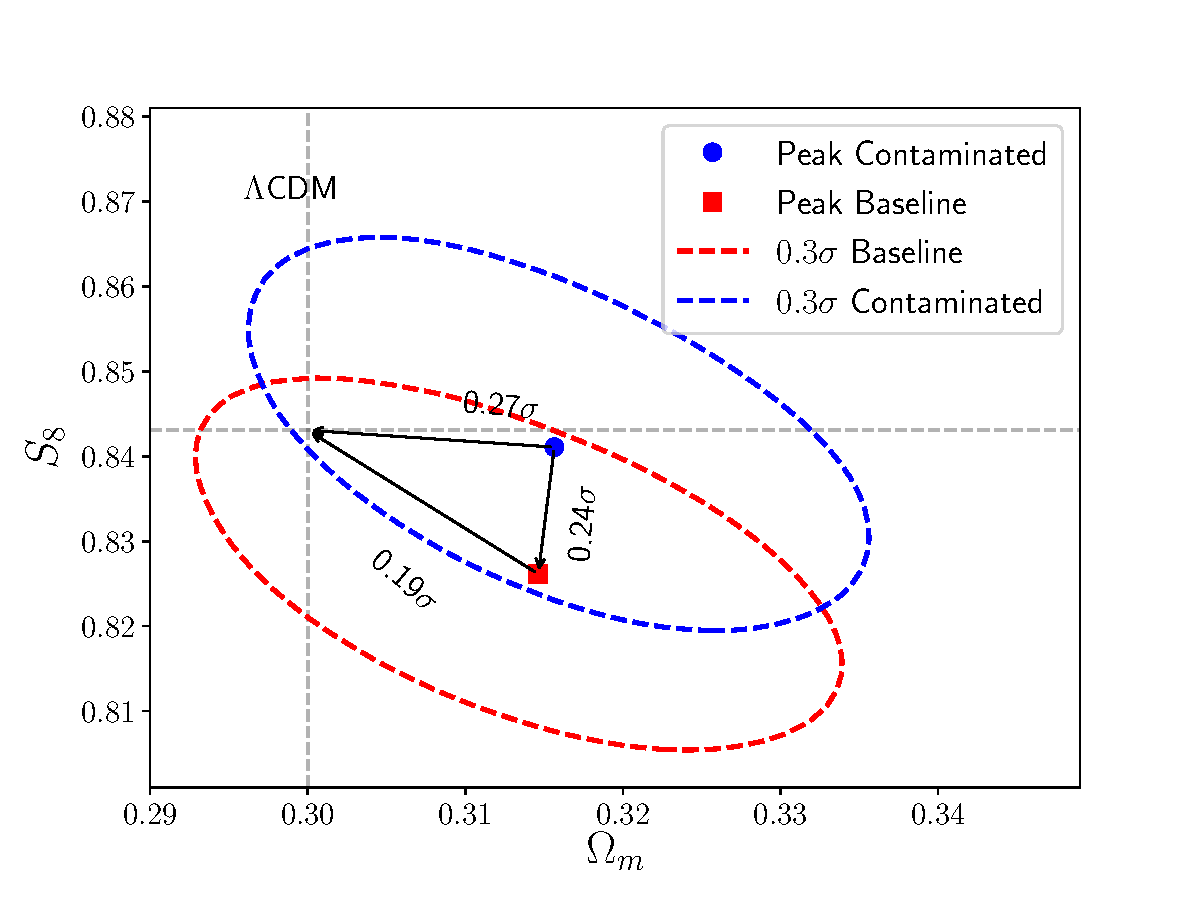
\includegraphics[width=0.49\textwidth]{figs/compare_cosmo_all_2x2pt_lcdm__v0.4_sc_8_6_0.5_OmS8_draftv1.pdf}
     }
\hfill
\subfloat{%
      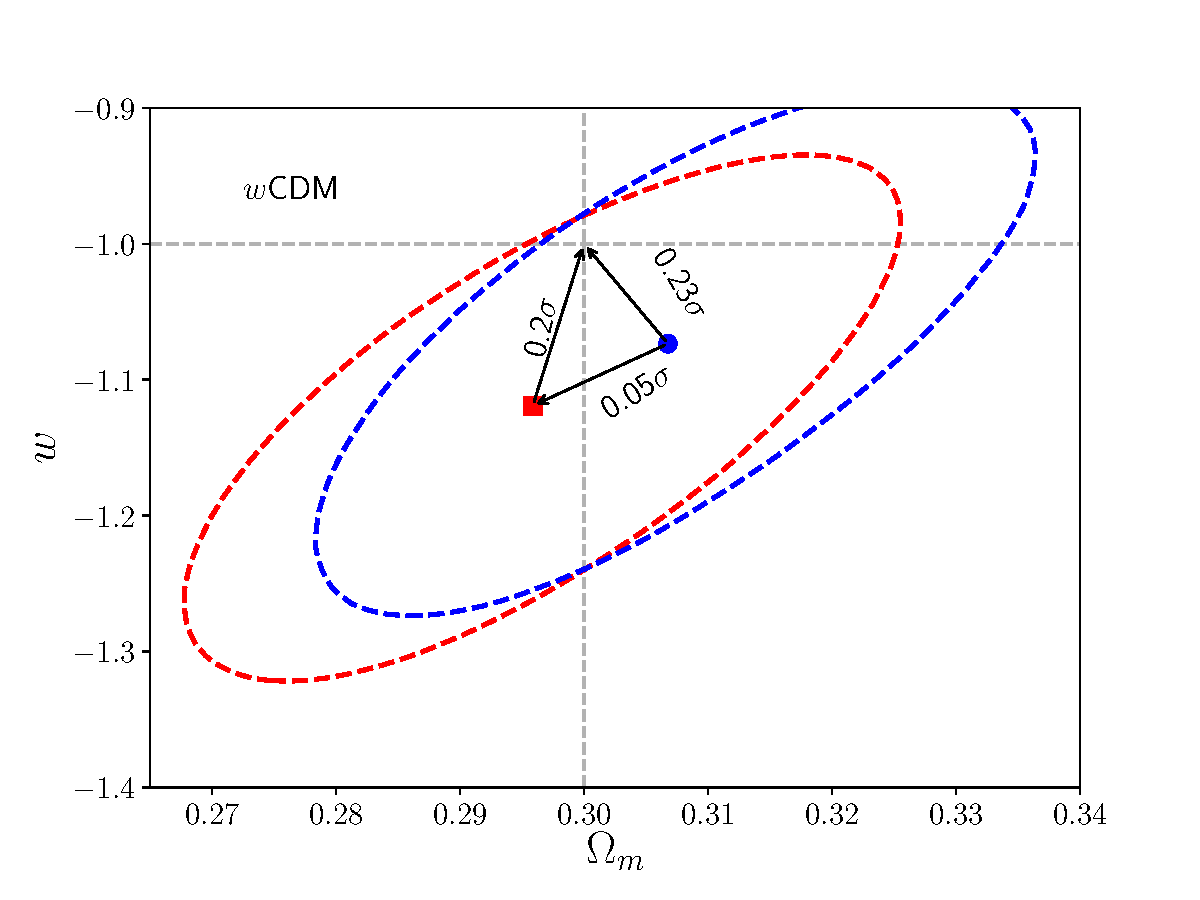
\includegraphics[width=0.49\textwidth]{figs/compare_cosmo_all_2x2pt_wcdm__v0.4_sc_8_6_0.5_Omw_draftv1.pdf}
     }
    \caption[]{Simulated datavector: parameter constraints from a datavector contaminated with non-linear bias + baryons but analyzed with a linear bias + halofit model. The left panel shows contours for \lcdm, and the right panel shows \wcdm. The scale cuts are (8,6) Mpc/$h$ for $w(\theta)$ and $\gamma_{\rm t}$ respectively. In both panels, we compare the peak of the marginalized constraints in the 2D  parameter plane for the contaminated datavector (blue circle) and the baseline datavector  (red square). We see that the distance between the peaks of marginalized baseline contours is within 0.3$\sigma$ of the marginalized contaminated contours, which is our criterion for acceptable scale cuts. }
\label{fig:sim_lin}    
\end{figure*}



\subsection{Results on Simulations}
\label{sec:sims}
Finally, we validate our model with mock catalogs from cosmological simulations for analysis choice combinations that pass the simulated likelihood tests. We use the suite of Y3 \buzzard simulations described above. We again require that our analysis choices return unbiased cosmological parameters. In order to reduce the sample variance, we analyze the mean datavector constructed from 18 \buzzard realizations. 
% \blue{We analyze the \mice simulations as well, but only one realization is available. The recovered cosmological contours and bestfit are shown in Appendix YYY}.

\subsubsection{Linear Bias Model}
We ran the simulated $2\times 2$-point analyses on the mean of the measurements from all 18 \buzzard simulations. We compare our model for $w(\theta)$ and $\gamma_{\rm t}(\theta)$ to our measurements at the true \textsc{Buzzard} cosmology, leaving only linear bias and magnification coefficients free. In this case, we have ten free parameters in total, and we find a chi-squared value of 13.6 for 285 data points using our \textit{fiducial} scale cuts (and assuming the covariance of a single simulation, as appropriate for application to the data). The analysis assumes true source redshift distributions and the fiducial model described in \S\ref{sec:sourcez}. Fixing the source redshift uncertainties to zero is a conservative choice; it results in cosmological constraints that have a probability to exceed a parameter bias of $0.3/1\sigma$ in the $S_8-\Omega_{\rm m}$ plane of 0.25/$<$0.01 and 0.35/$<$0.01 in the $w-\Omega_{m}$ plane. A similar analysis, using calibrated photometric redshift (and their uncertainties) shows a probability to exceed a parameter bias of $0.3/1\sigma$ in the $S_8-\Omega_{m}$ plane with respect to the true redshift analysis of 0.08/$<$0.01, and 0.05/$<$0.01 in the $w-\Omega_{m}$ plane.

\blue{Make the case about projection effects being different for wcdm baseline compared to simulated DV analysis in previous section. i.e. projection effects are dependent upon the parameter values.}

\subsubsection{Scale cuts for non-linear bias}
% \IR{The scale cuts for non-linear bias will be finalized...For all of the tests that we have done, (4,4)Mpc/h cut passes our criterion. }
Likewise, we have run simulated $2\times 2$-point analyses, including our non-linear bias model on the mean of the measurements from all 18 simulations. Similar to the procedure used to determine the linear bias scale cuts in \S\ref{sec:sc_linbias}, we iterate over scale cuts for each tomographic bin defined from varying physical scale cuts. We find that angular scale cuts corresponding to (4,4) Mpc/$h$ for $\wtheta$ and $\gammat$ pass our threshold scale cut criteria.  

We compare our model for $w(\theta)$ and $\gamma_{\rm t}(\theta)$ to our measurements at the true \textsc{Buzzard} cosmology, leaving our bias model parameters and magnification coefficients free, which add 15 free parameters. We find a $\chi^2$ value of 15.6 for 340 data points using our non-linear bias scale cuts and assuming the covariance of a single simulation. Simulated analyses using true redshift distributions result in cosmological constraints that have a probability to exceed a parameter bias of $0.3/1\sigma$ in the $S_8-\Omega_{m}$ plane of 0.20/$<$0.01 and 0.26/$<$0.01 in the $w-\Omega_{m}$ plane.


\begin{figure*}
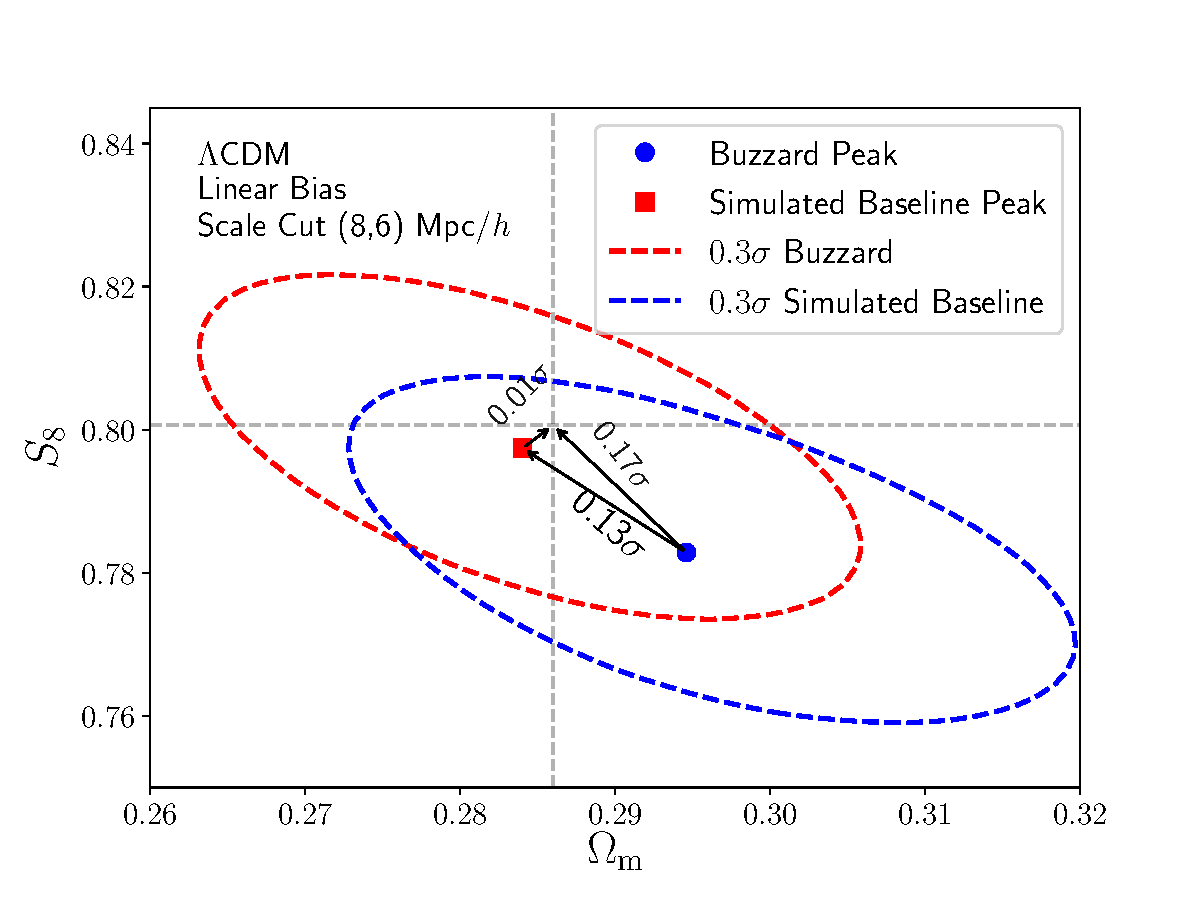
\includegraphics[width=\columnwidth]{figs/Buzzard_linbias86_2x2pt_lcdm.pdf}
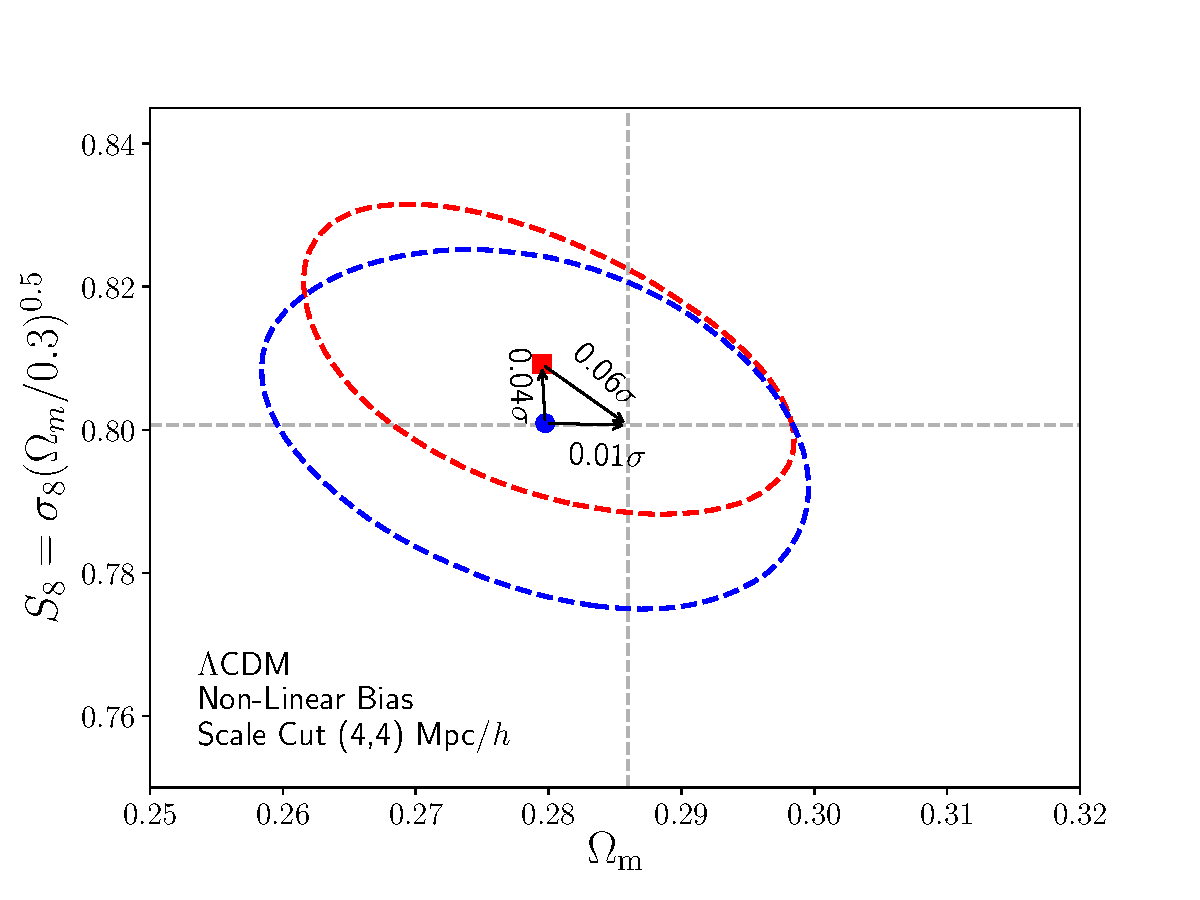
\includegraphics[width=\columnwidth]{figs/Buzzard_nlbias44_2x2pt_lcdm.pdf}
\caption[]{The blue contours show constraints from \buzzard simulations (blue contours) compared with  \buzzard-like theory datavector (red contours) in the $\Lambda$CDM cosmological model.
%The blue contours correspond to the result from the mean (over all Y3-like realizations) of Buzzard 2x2pt measurements, with covariance corresponding to single realization. 
The left (right) panel shows the constraints for linear (non-linear) bias models with the scale cuts given in the legend. The linear and non-linear bias values are extracted from fits to the 3D correlation functions ($\xigg$ and $\xigm$). We see that both the scale cut choices satisfy our validation criterion. 
% \IR{we will update these plots with all 18 realizations in Y3 settings including varying neutrino masses}
}
\label{fig:bcc_des_lcdm}
\end{figure*}

In \fig{fig:bcc_des_lcdm} we show the constraints on $\Omega_{\rm m}$ and $S_8$ from the mean Buzzard $2\times2$pt measurements for \lcdm. The results for the linear and non-linear bias models are shown, and again, the criterion for unbiased cosmology is satisfied for the fiducial choice of scale cuts. 
\fig{fig:bcc_des_wcdm} shows the same analysis for $\Omega_{\rm m}$ and $w$.



\begin{figure*}
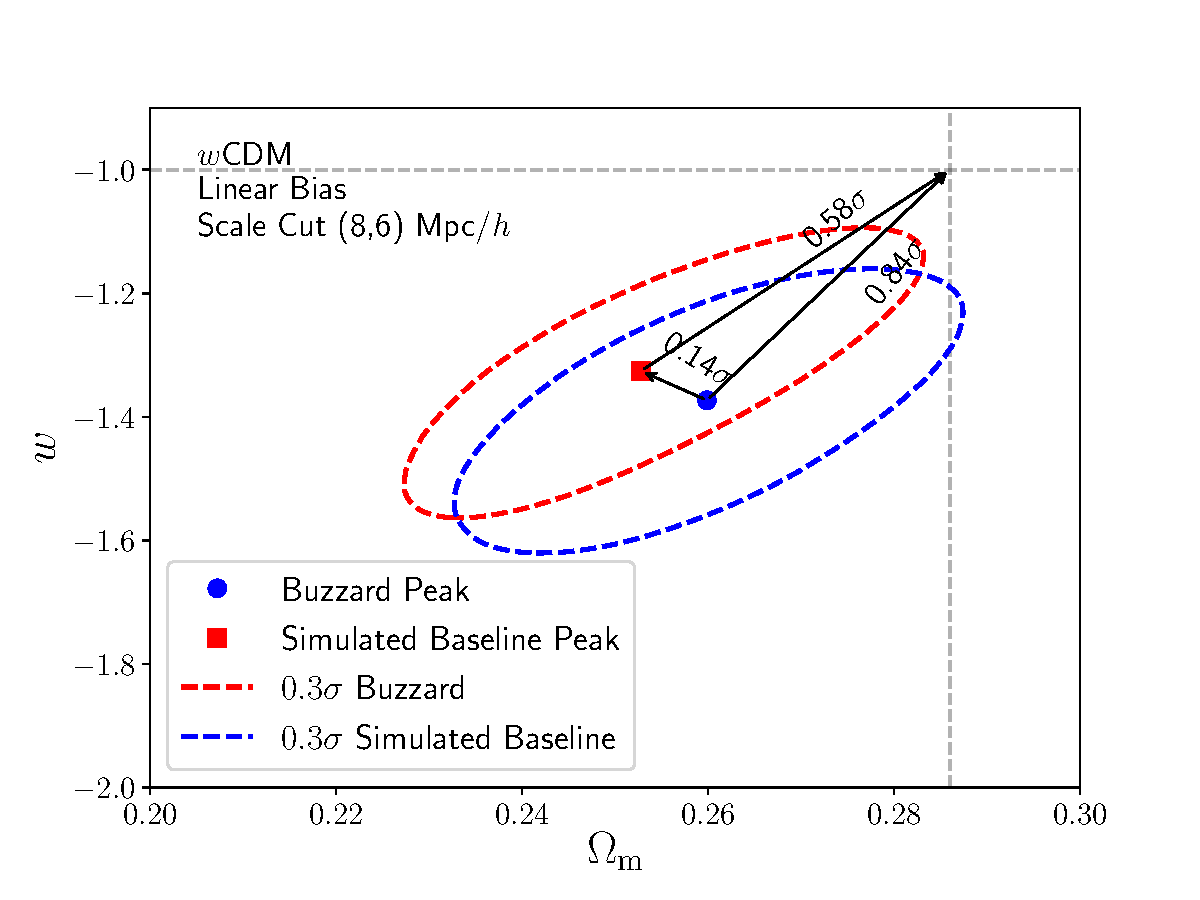
\includegraphics[width=\columnwidth]{figs/Buzzard_linbias86_2x2pt_wcdm.pdf}
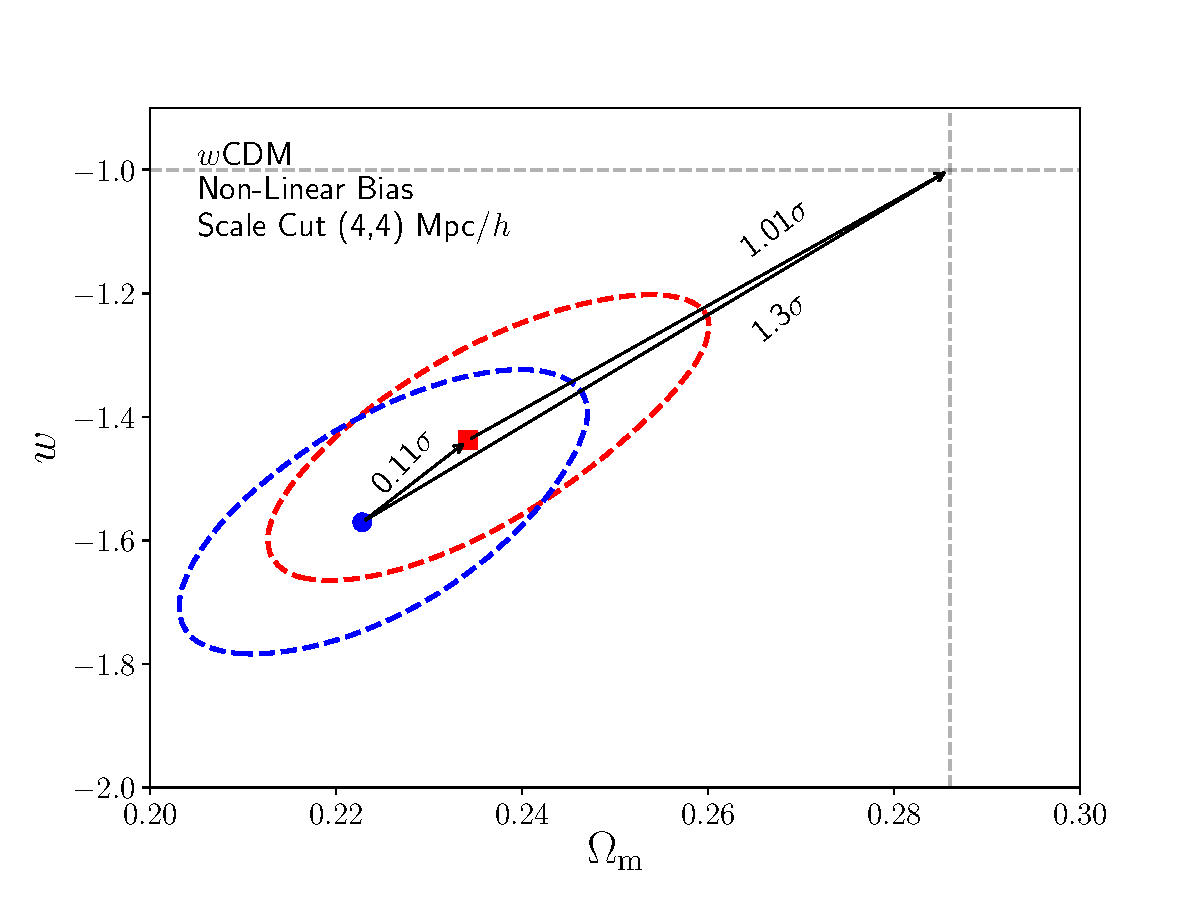
\includegraphics[width=\columnwidth]{figs/Buzzard_nlbias44_2x2pt_wcdm.pdf}
\caption[]{Same as Fig.~\ref{fig:bcc_des_lcdm} but for $w$CDM cosmology.
}
\label{fig:bcc_des_wcdm}
\end{figure*}


\section{Results}

\subsection{Cosmology constraints}

In Fig.~\ref{fig:des_comp}, we compare the constraints on the cosmological parameters obtained from jointly analyzing $\wtheta$ and $\gammat$ with both linear and non-linear bias models. We find $\om = 0.325^{+0.033}_{-0.034}$ from the linear bias model at our fiducial scale cuts, while using the non-linear bias for same scale cuts gives us $\om = 0.3^{+0.035}_{-0.037}$. We also show the results for the scale cuts of (4,4) Mpc/$h$ using the non-linear bias model where we find $\om=0.323^{+0.034}_{-0.035}$. These marginalized constraints on $\om$ are completely consistent with the DES-Y1 results and \Planck results. 

With our fiducial analysis of linear bias model with (8,6) Mpc/$h$ scale cuts, we find $S_8 = 0.668^{+0.026}_{-0.033}$. As is evident from the contour plot in Fig.~\ref{fig:des_comp}, our constraints prefer lower $S_8$ compared to previous analyses.  We use the Monte-Carlo parameter difference distribution methodology (as detailed in \cite{y3-tensions}) to assess the tension between our fiducial constraints and \Planck results. Using this criterion, we find a tension of 4.1$\sigma$, largely driven by the differences in the $S_8$ parameter. We find similar constraints on $S_8$ from the non-linear bias as well for both our scale cuts. We investigate the cause of this low $S_8$ value in the following sub-sections. 

Note that non-linear bias model at (4,4)Mpc/$h$ scale cuts results in tighter constraints in the $\om-S_8$ plane. We estimate the total constraining power in this $\om-S_8$ plane by integrating the marginalized posterior for each model. 
% We find that non-linear bias model at  (4,4)Mpc/$h$ results in the value of $0.005226$. In comparison, linear bias at (8,6)Mpc/$h$ results in a value of $0.00613$; therefore non-linear bias model results in a $14.8$\% increase in constraining power. 
We find that non-linear bias model at  (4,4)Mpc/$h$ results in a $14.8$\% increase in constraining power compared to linear bias at (8,6)Mpc/$h$. 


\begin{figure}
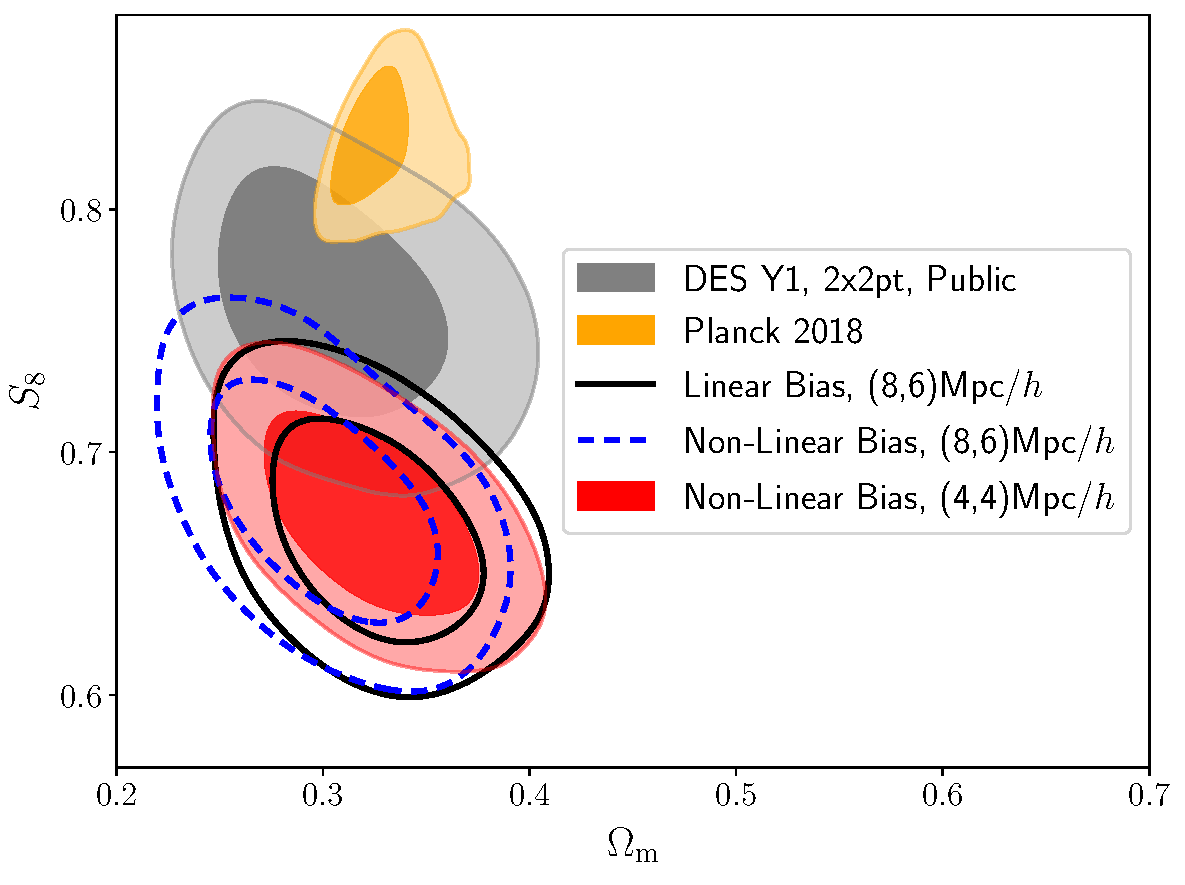
\includegraphics[width=\columnwidth]{figs/data_lcdm_comp.pdf}
\caption[]{Comparison of the $2\times2$pt $\Lambda$CDM constraints for both linear bias and non-linear bias at their respectively defined scale cuts given in the legend. We find a preference for low value of $S_8$ with both models of galaxy bias which we investigate in \S\ref{sec:internal_consistency}. We also show that using non-linear bias leads to better constraints in the $\Omega_{\rm m} - S_8$ plane. }\label{fig:des_comp}
\end{figure}

\subsection{Comparison with Maglim results}
In \citet{y3-2x2ptaltlensresults} we analyze an alternative magnitude limited lens sample and present the results obtained from a $2\times2$pt analysis of that. We find that that sample gives consistent results with the DES Y1 results. This also suggests some lingering systematic rather than some physical process happening with the \redmagic sample.  
\subsubsection{Non-linear bias results on Maglim}
% \blue{Refer to the 3D residuals in Buzzard sims plot in the appendix.}
We also show the constraints obtained from the non-linear bias analysis on the Maglim sample in Fig.~\ref{fig:maglim_comp}. 


\begin{figure}
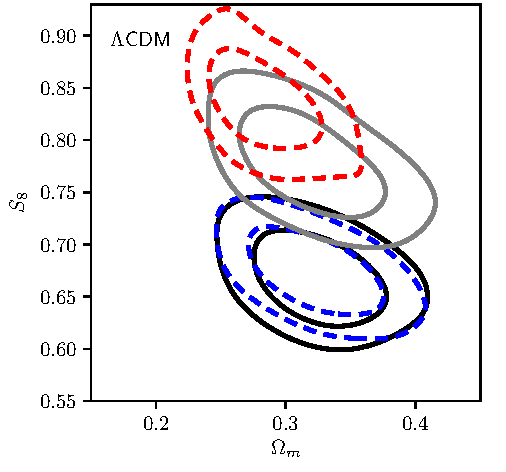
\includegraphics[width=\columnwidth]{figs/compare_maglim_rm_lcdm.pdf}
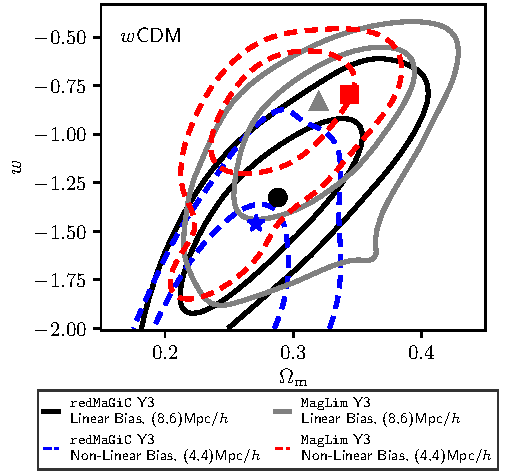
\includegraphics[width=\columnwidth]{figs/compare_maglim_rm_wcdm.pdf}
% \vfil
% 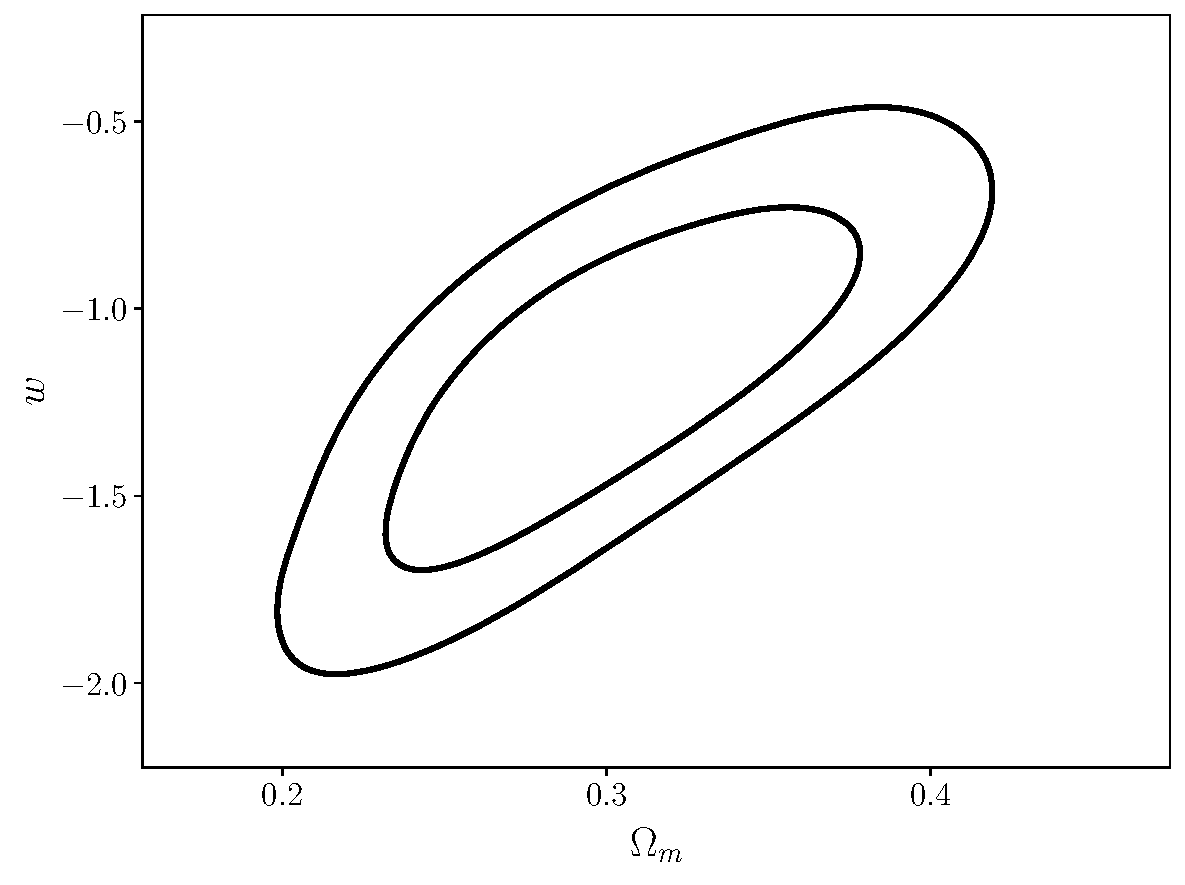
\includegraphics[width=\columnwidth]{figs/data_wcdm_comp.pdf}
\caption[]{Comparing the constraints from $2\times2$pt between \redmagic and Maglim sample. \IR{The Maglim Non-linear bias (4,4) chain is old one with using all six tomographic bins. The one with four bins is still running.}}\label{fig:maglim_comp}
\end{figure}




\subsection{Internal consistency of the cosmology results}
\label{sec:internal_consistency}

To investigate the low $S_8$ constraints from our fiducial analysis, we first check various aspects of our modeling pipeline. We show summary constraints on $\om$, $S_8$ and galaxy bias for third tomographic bin $b_3$ in Fig.~\ref{fig:2x2pt_consistency}. We divide the figure into three parts, separated by horizontal black lines. The top panel shows the marginalized constraints from the results described in the previous subsection (see Fig.~\ref{fig:des_comp}). As mentioned previously, we obtain completely consistent constraints from both linear and non-linear bias models. To check the robustness and keep the interpretation simple, we use the linear bias model using the scale cuts of (8,6)Mpc/$h$ in the following variations.  

In the next part of the figure, we test the robustness of the model. In particular, we check the robustness of our fiducial intrinsic alignment model by using the NLA model. We also run our analysis by fixing the neutrino masses to $\Omega_{\nu}h^2 = 0.00083$. Lastly, we test the impact of varying the dark energy parameter using $w$CDM model. We find entirely consistent constraints for all of the above variations. 

In the next part of the figure, we test the robustness of parts of our datavector. Firstly we remove the contribution of shear-ratio information in our likelihood, resulting in completely consistent constraints. Also, note that the constraints on the cosmological parameters do not change in this case compared to our fiducial constraints, which shows that most constraints on cosmological and bias parameters are obtained from the $\wtheta$ and $\gammat$ themselves. We also test the impact of removing one tomographic bin at a time from our datavector. We find consistent constraints in all five cases, demonstrating that no single tomographic bin drives the constraints on $S_8$ to a low value. Lastly, we also dissect the datavector into large and small scales. The small scales run only analyzes the datavector between the angular scales corresponding to (8,6)Mpc/$h$ and (30,30)Mpc/$h$. The large scales run analyzes the datavector between angular scales corresponding to (30,30)Mpc/$h$ and 250 arcmin. When analyzing the large scales, we also remove the point-mass marginalization from our analysis. In both cases, we find similar constraints, demonstrating that the low $S_8$ is not originating from either large or small scales.

Finally, to check the robustness of our pipeline, we analyze the $\wtheta$ and $\gammat$ measurements as measured from DES Y1 data \citet{Abbott_2018}. Note that in this analysis, we keep the same scale cuts as described and validated in \citet{Abbott_2018, MacCrann2018}, which are $8$Mpc/$h$ for $\wtheta$ and $12$Mpc/$h$ for $\gammat$. To analyze this datavector, while we use the model described in this paper, we fix the point-mass parameters to zero because of the large degradation of constraining power at these larger-scale cuts due to degeneracy between point-mass parameters, galaxy bias and cosmological parameter $\sigma_8$. We compare these constraints to the public results as described in \citet{Abbott_2018}, finding that we obtain consistent constraints with our pipeline.

Lastly, to assess the impact of the projection effect on the $S_8$ parameter, we compare the profile posterior to the marginalized posterior. The profile posterior is obtained by calculating the maximum posterior value for a given value of $S_8$. Therefore, unlike marginalized posterior, the profile posterior does not involve the projection of high dimensional posterior to a single $S_8$ parameter. Hence the histogram of the profile posterior is not impacted by projection effects. We compare the marginalized posterior and profile posterior in Fig.~\ref{fig:prof_like}, demonstrating that projection effects do not impact the inferred $S_8$ constraints from the marginalized posterior.  
 
These results demonstrate that our methodology pipeline is completely robust, and it is our data that is resulting in low $S_8$ constraints. Moreover, as described above, no individual part of our data drives a low value of $S_8$; therefore we perform global checks of our datavector in the following sections.


\subsection{Galaxy bias from individual probes at fixed cosmology}

In this sub-section, we test the compatibility of $\wtheta$ and $\gammat$ part of our datavector. As we will lose the complementarity when analyzing  $\wtheta$ and $\gammat$ parts of datavector individually, we fix the cosmological parameters to the maximum posterior obtained from \citet{Abbott_2018}. We find that the best-fit bias values from $\wtheta$ part of our datavector are systematically higher than $\gammat$ for each tomographic bin. We parameterize this difference in bias values with a parameter $X^{i}_{\rm lens}^i = b^i_{\gammat}/b^i_{\wtheta}$. The constraints on the parameter $X^{i}_{\rm lens}^i$ are shown in Fig.YYY. We also compare the constraints 


Note that, for this choice of cosmological parameters, our datavector value of $X^{i}_{\rm lens}^i \sim 0.85$ for each bin at high confidence. Therefore, in order to keep the interpretation simple, we use a single parameter $X_{\rm lens}$ to describe the ratio of galaxy bias $b^i_{\gammat}/b^i_{\wtheta}$ for all tomographic bins $ i \in [1,5]$.  


\begin{figure*}
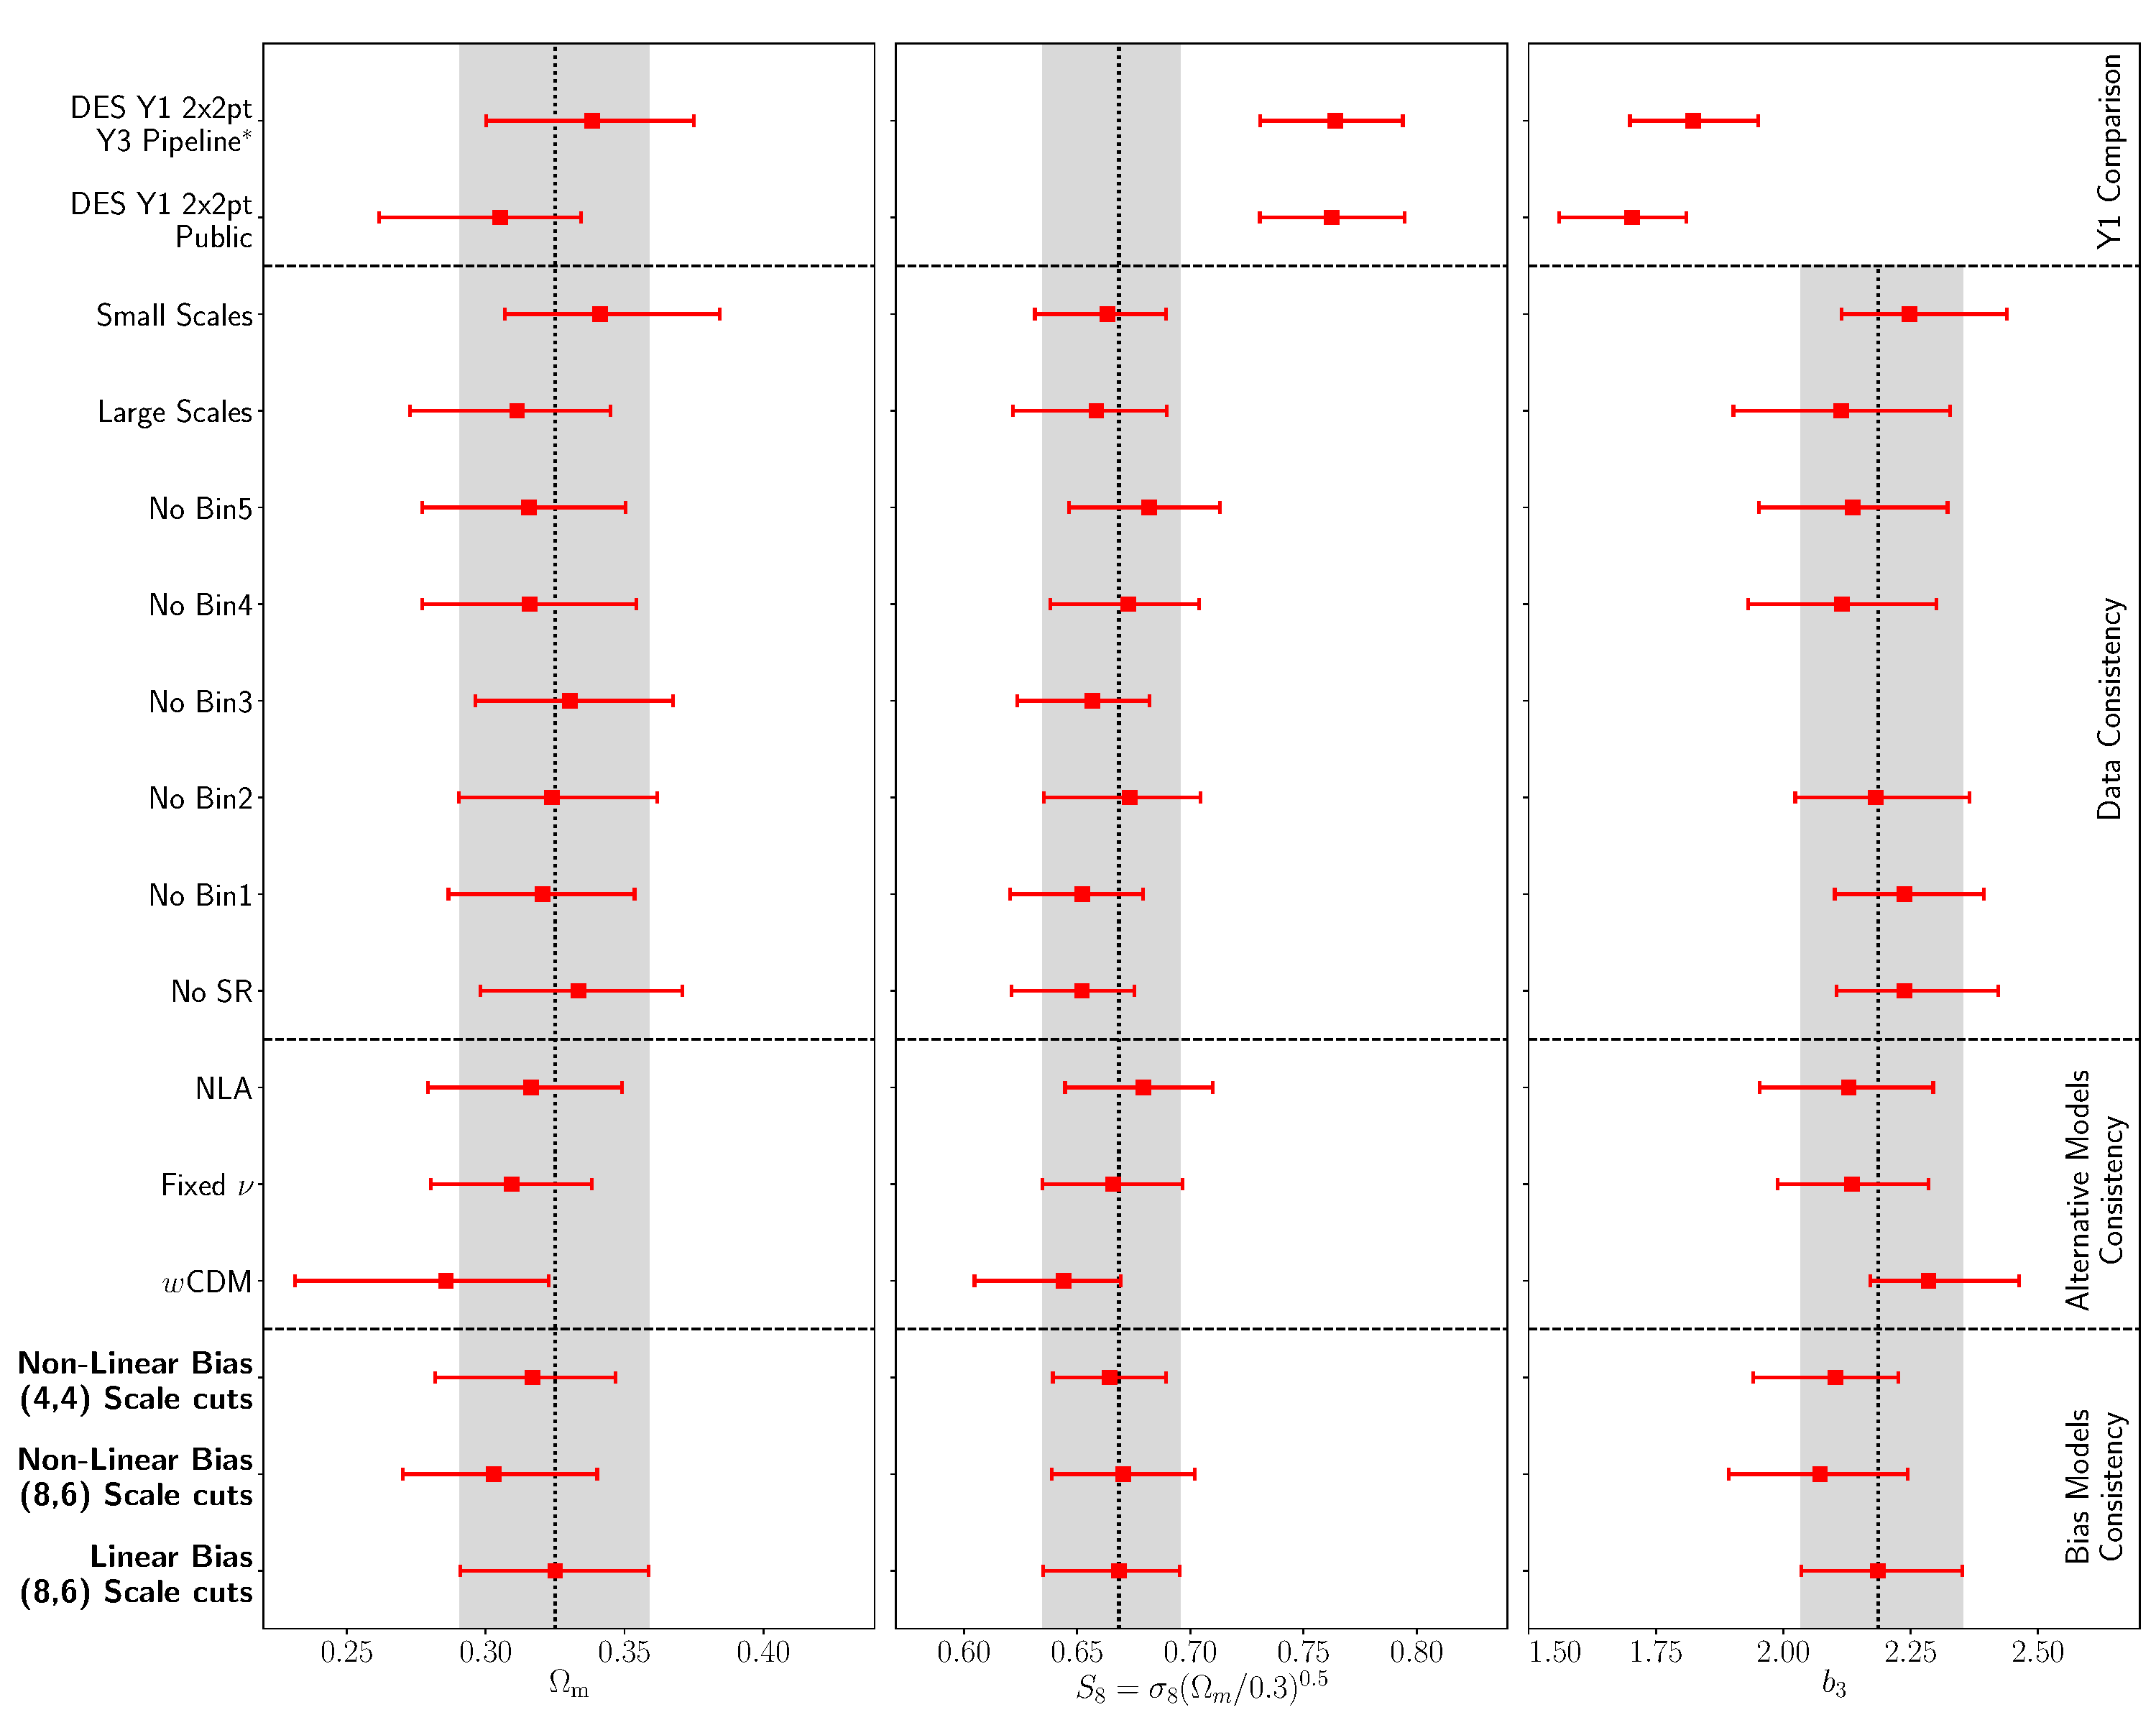
\includegraphics[width=\textwidth]{figs/2x2pt_consistency.pdf}
\caption[]{DATA: The figure shows the consistency of the $2\times2$pt constraints. \blue{maybe replace the sigma8 in last panel with $b_3$(highest constrained bias parameter)?} }
\label{fig:2x2pt_consistency}
\end{figure*}

\begin{figure}
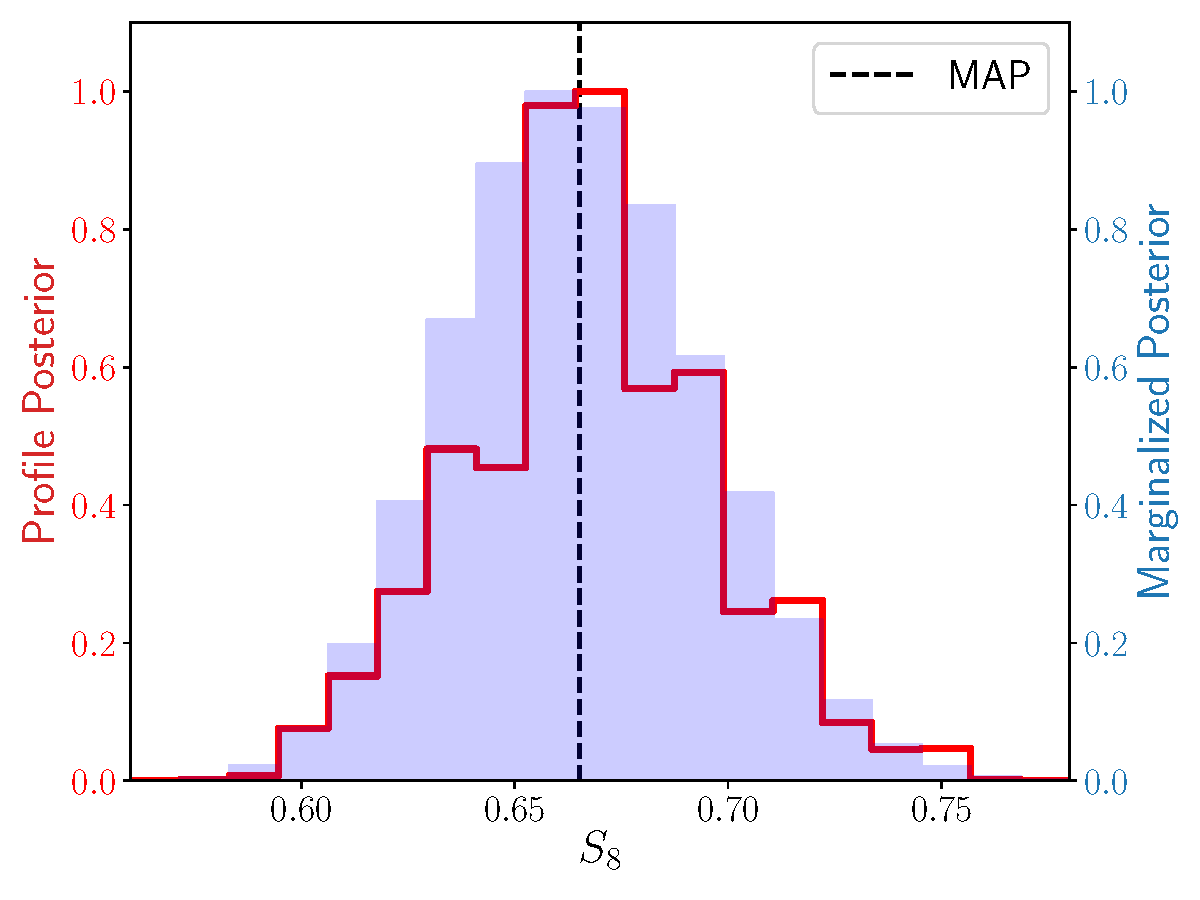
\includegraphics[width=\columnwidth]{figs/profile_likelihood_emcee.pdf}
\caption[]{The comparison of the profile posterior and marginalized posterior on $S_8$ parameter from the $2\times2$pt \redmagic LCDM chain}
\label{fig:prof_like}
\end{figure}



\subsection{Is lensing low?}
\label{sec:boss_x}
% \blue{Which external datasets to include?}
In this section, we try to identify which particular part of our datavector, $\wtheta$ or $\gammat$, is driving $X_{\rm lens} \neq 1$. To that end, we correlate our lens galaxy sample with BOSS/eBOSS catalogs. There is a 650 square degrees of overlap between the DES Y3 and BOSS survey. As the BOSS galaxies have a spectroscopic redshift assignment with negligible uncertainty, we divide that sample into finer tomographic bins. The sample is split into 10 tomographic bins, two sub-bins within each of five DES lens galaxy sample tomographic bins. We then measure the correlations between the \redmagic and \maglim galaxies in each bin with the BOSS galaxies corresponding to each sub-bin. We parameterize the power spectrum of auto-correlations between the external BOSS galaxies ($P_{\rm ee}$) and cross-correlations between BOSS and DES lens galaxies ($P^{\rm RM}_{\rm eg}$, for \redmagic and $P^{\rm Mag}_{\rm eg}$ for \maglim) as: $P_{\rm ee} = b^2_{\rm e} P_{\rm mm}$, $P^{\rm RM}_{\rm eg} = X_{\rm BOSS} X_{\rm lens, RM} b_{\rm e} b_{\rm g} P_{\rm mm}$ and $P^{\rm Mag}_{\rm eg} = X_{\rm BOSS} X_{\rm lens, Mag} b_{\rm e} b_{\rm g, Mag} P_{\rm mm}$. The power spectra of the auto-correlations of the DES galaxies, $P^{\rm RM}_{\rm gg}$ and $P^{\rm Mag}_{\rm gg}$ for \redmagic and \maglim respectively are described in \S\ref{sec:Pk_pred}. The final two-point correlations are then obtained from these power spectrum using the framework described in \S\ref{sec:proj_2pt}. Note that we neglect the corrections from non-limber and RSD in the cross-correlations between BOSS and \redmagic catalogs, because of smaller signal-to-noise as these measurements are limited to only 650 square degrees. We have validated that the impact from these is significantly smaller than our errorbars in these measurements, giving $\Delta \chi^2 = YYY$. The covariance between them is a Gaussian covariance using the code described in \S\ref{sec:cov}. We now jointly analyze the three two-point projected angular correlations constructed from DES lens galaxies and BOSS galaxies. The details of the measurement methodology is shown in Appendix.


In Fig.~\ref{fig:X_comp_main}, we compare the marginalized posterior on $X_{\rm lens}$ parameter from this BOSS cross-correlations with the result from analyzing $2\times2$pt datavector from DES Y3 or DES Y1. We find that while DES Y1 is completely consistent with $X_{\rm lens} = 1$, both DES Y3 $2\times2$pt and Y3xBOSS prefer similar low value of $X_{\rm lens}$. Note that all these contours fix the cosmological parameters to the maximum posterior from \citet{Abbott_2018}. This suggests that our datavector has a preference for high auto-correlation of galaxies, and the cross-correlations prefer lower bias values. We refer the readers to \citet{y3-galaxyclustering} for more tests related to clustering of \redmagic galaxies. 


We note some of the approximations and caveats in the above test. This test assumes that the weights of \redmagic galaxies are the same even when there is only a partial overlap between the full Y3 area and BOSS area. We also assume that the BOSS area and full DES Y3 area have the same galaxy number density parameterization. We leave a more careful analysis of the cross-correlations to future work. 

\begin{figure}
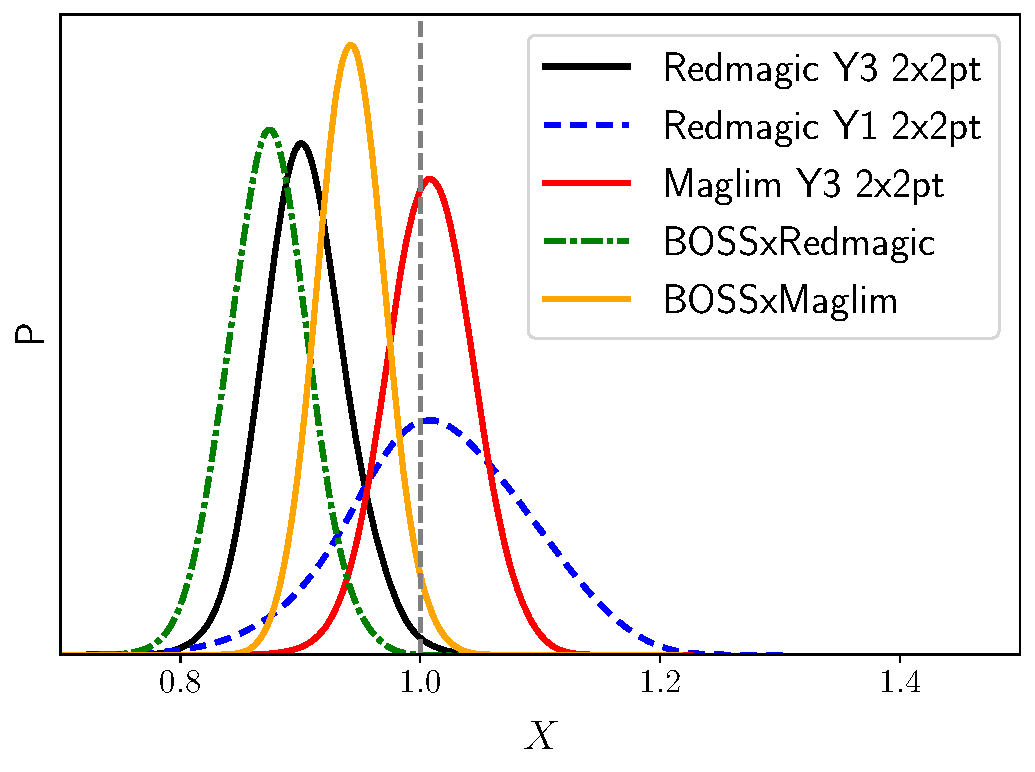
\includegraphics[width=\columnwidth]{figs/X_comp_bossrm_y3.pdf}
% \vfil
% 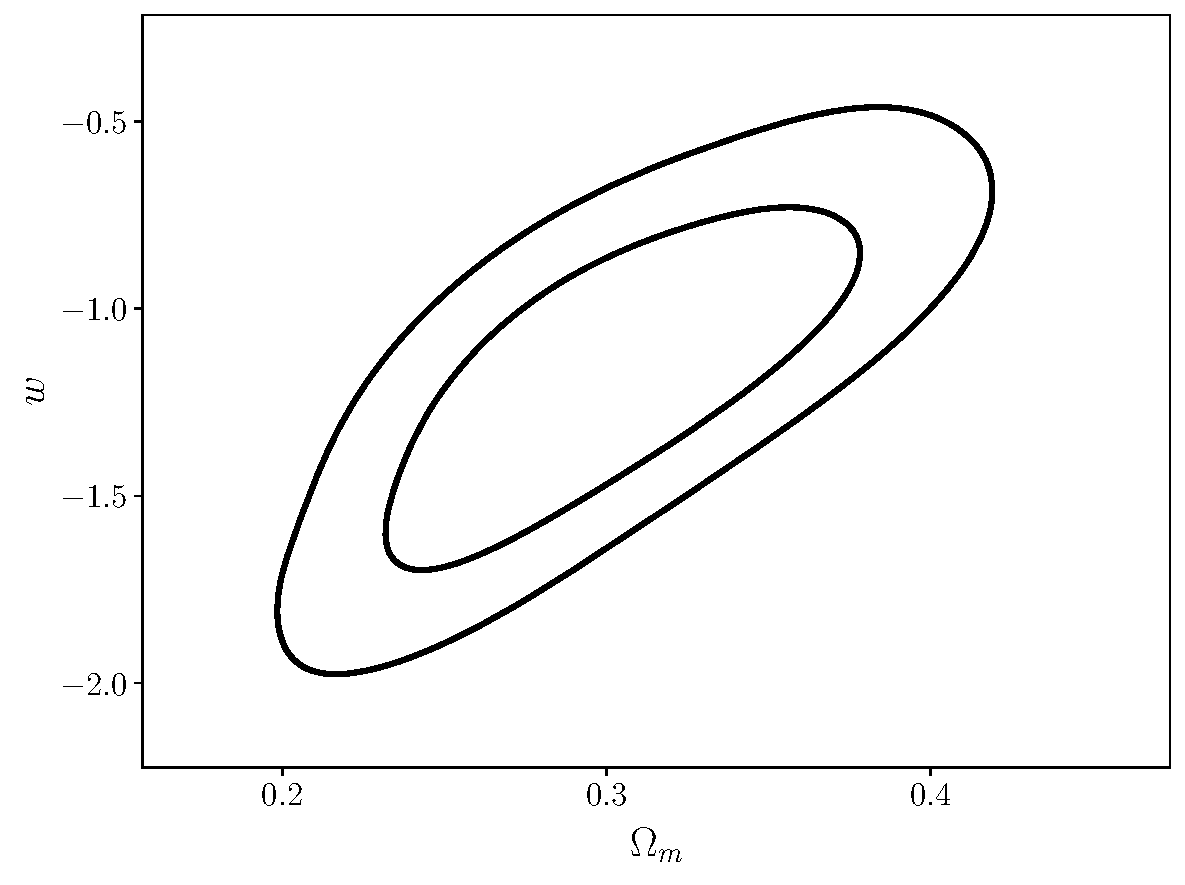
\includegraphics[width=\columnwidth]{figs/data_wcdm_comp.pdf}
\caption[]{Comparison of the decorrelation parameter ($X_{\rm lens}$), ratio of bias of \redmagic estimated from cross-correlations and its auto-correlation ($\wtheta$). We compare the posterior on $X$ when using either BOSS$\times \redmagic$ or $\gammat$ and find consistent posteriors.  }\label{fig:X_comp_main}
\end{figure}


\begin{figure}
\includegraphics[width=\columnwidth]{figs/data_lcdm_wX_{\rm lens}_comp.pdf}
% \vfil
% 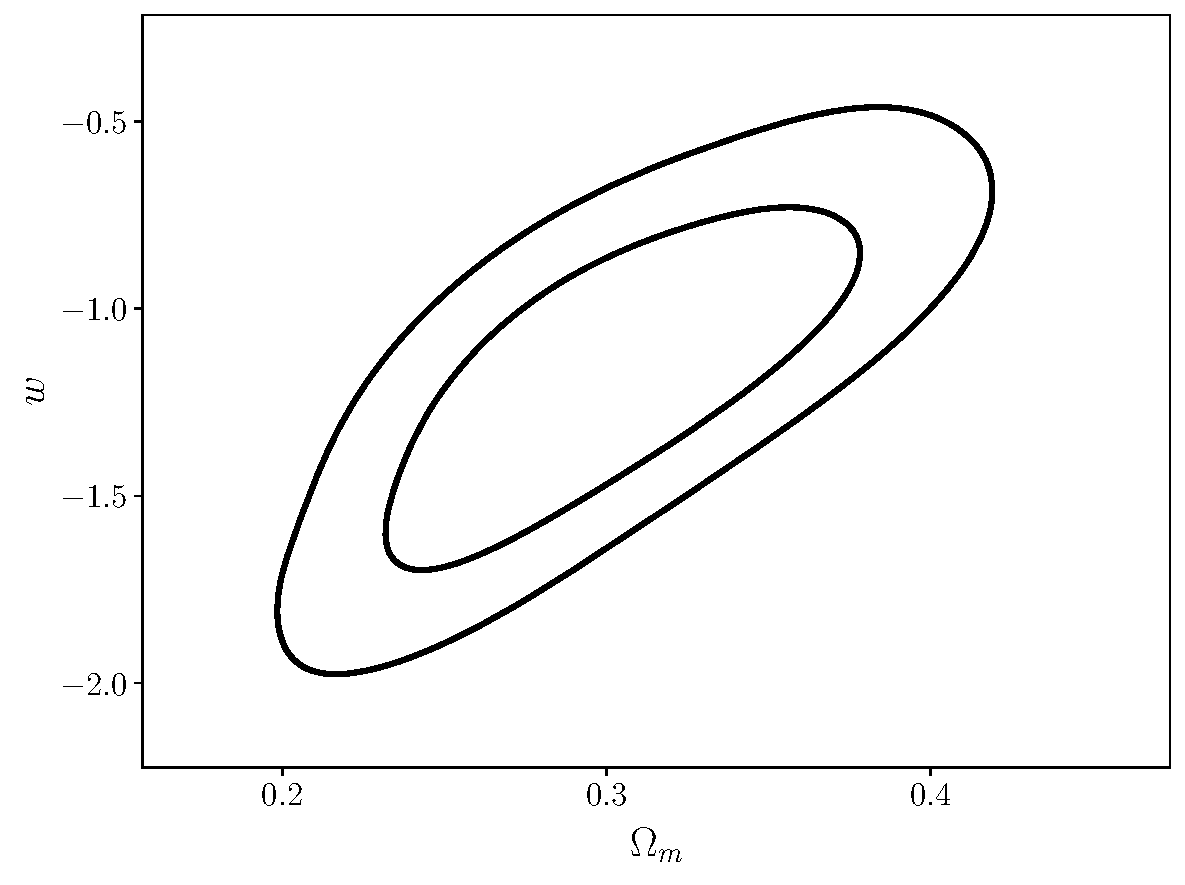
\includegraphics[width=\columnwidth]{figs/data_wcdm_comp.pdf}
\caption[]{Comparing the constraints from $2\times2$pt when correcting the datavector with the mean value of decorrelation parameter.  }\label{fig:X_comp_main}
\end{figure}


% \subsubsection{Results}




\subsection{Halo mass inference}

We show the constraints on linear bias parameters for five tomographic lens bins in the left panel of Fig.~\ref{fig:bias_mass_nbar}. We can use these bias constraints and the constraints on co-moving number density to infer the mean host halo mass of our lens galaxy sample. We use a halo model framework and marginalize over the unknown halo model parameters to make a robust inference. The details of the halo model framework used here are given in Appendix \ref{app:halo_mass}. Note that we have neglected the effects of assembly bias in this analysis and the correlation between number density and bias constraints. With these caveats in mind, we report approximately 25\% constraints on mean host halo mass for our five tomographic bins.

\blue{We also use the wtheta * X bias value and the fiducial bias values (with corresponding cosmology), to infer the constraints on the halo masses of our galaxies. }


\begin{figure}
% 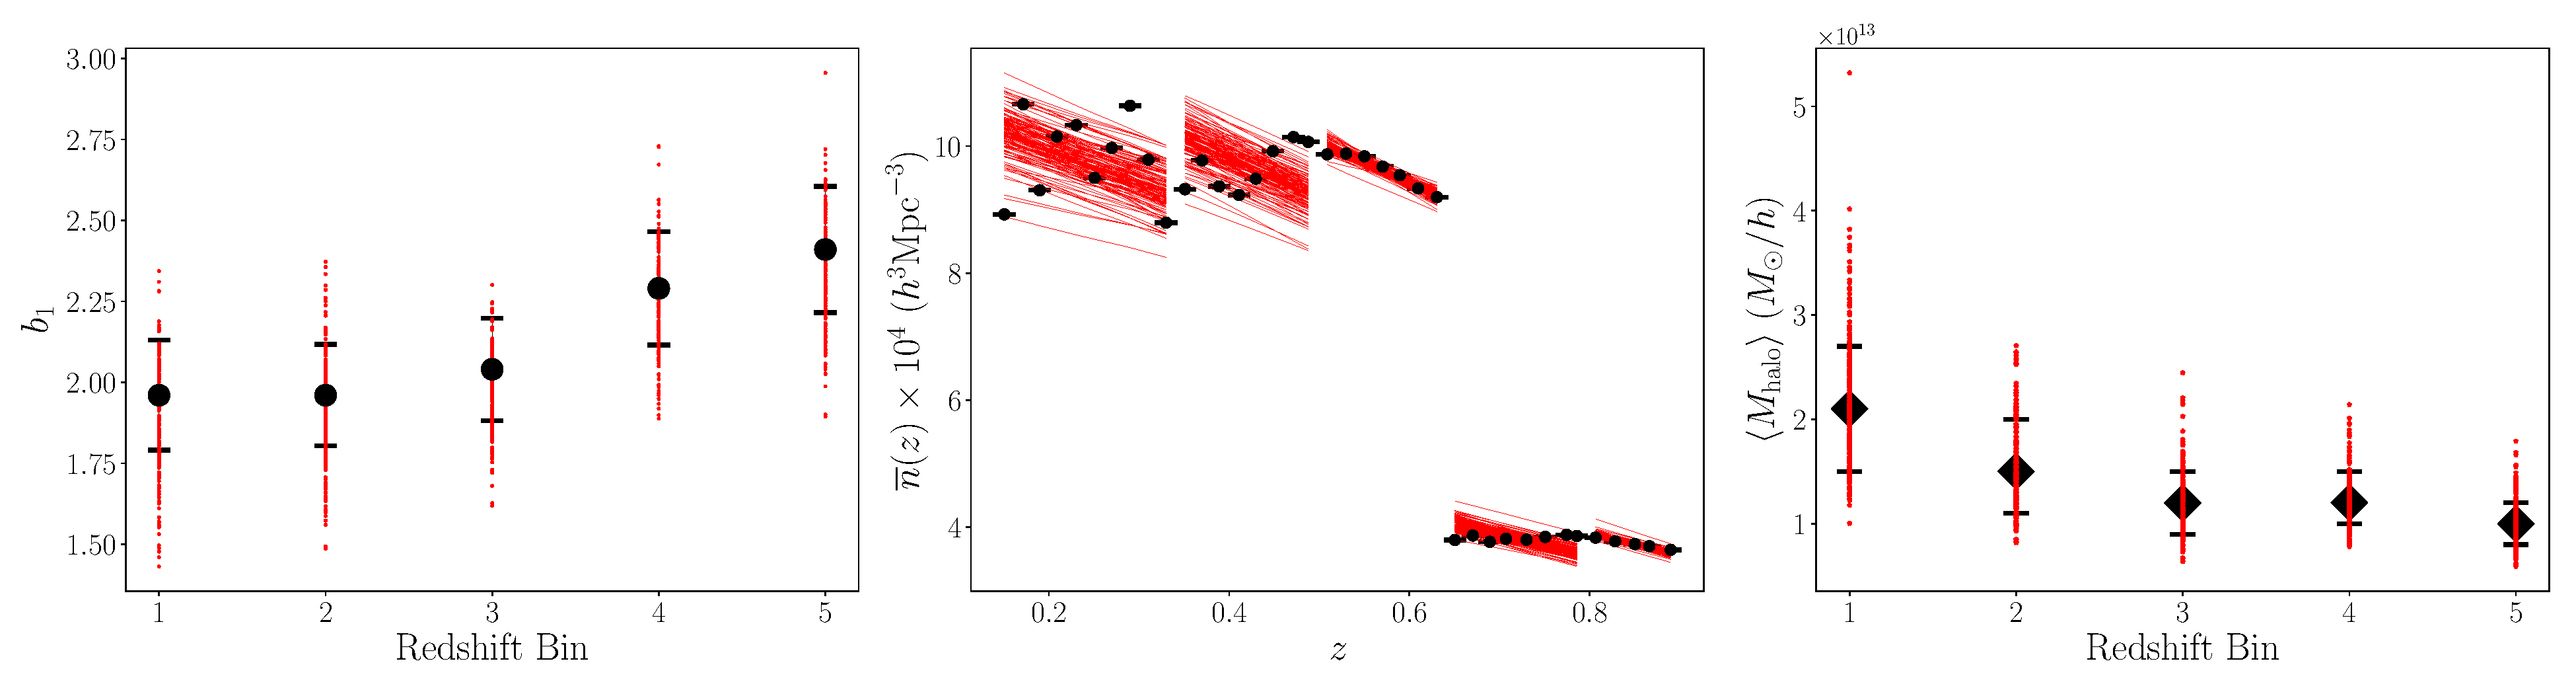
\includegraphics[width=\textwidth]{figs/b1_nbar_Mh_sim_marg_wcov.pdf}
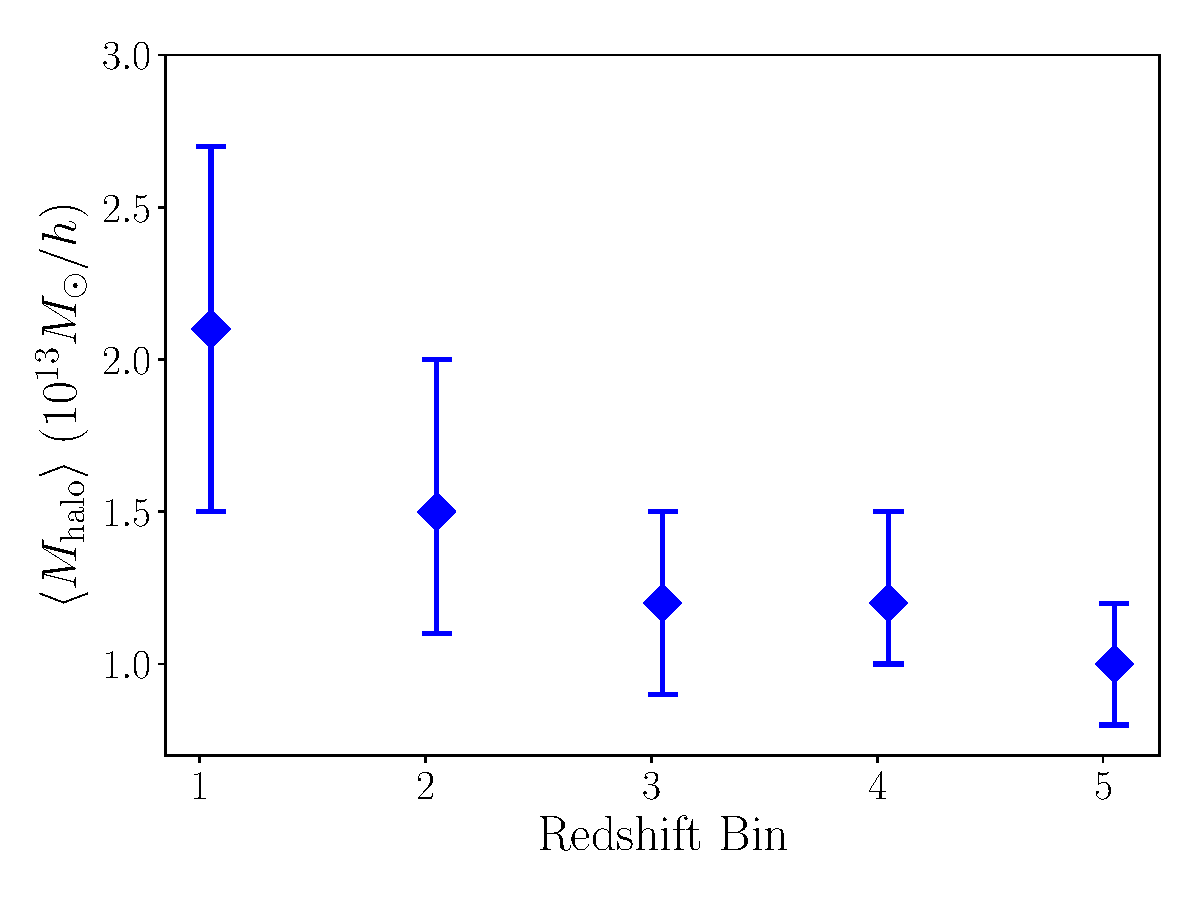
\includegraphics[width=\columnwidth]{figs/M_const.pdf}
\caption[]{DATA: This figure shows the marginalized constraints on the large-scale bias for the five tomographic bins on the left panel. The black dots denote the mean, and the error bars correspond to 16th and 84th percentile, respectively. Using this and co-moving number density (middle panel), we infer the constraints on mean halo mass, as shown in the right panel for five tomographic bins. We use the HOD framework to make this inference as detailed in Appendix \ref{app:halo_mass}. \blue{Make this a single panel figure only showing the halo masses constraints, but for fiducial linear bias chain as well as one with an X-prior run. }
}
\label{fig:bias_mass_nbar}
\end{figure}

% \subsection{Non-linear bias parameter constraints}


\section{Conclusions}

This paper has presented the cosmological analysis of the $2\times2$pt datavector of the DES Year 3 dataset. The $2\times2$pt datavector comprises the 2-point correlations of galaxy clustering and galaxy lensing using five redshift bins for the lens galaxies and four bins for source galaxies. It provides independent constraints on the two primary parameters of interest, the mass density $\Omega_{\rm m}$ and amplitude of fluctuations $S_8$. As shown in Fig.~\ref{fig:all2pt_comp}, these constraints are complementary to those from cosmic shear. The combination is thus better able to constrain $\Omega_{\rm m}, S_8$ as well as the dark energy equation of state parameter $w$. Perhaps more importantly, this provides a robustness check on the results from either approach. 

The estimation and marginalization of galaxy bias parameters is one of central tasks in extracting cosmology from the $2\times2$pt datavector. We have developed and validated the methodology for this based on perturbation theory. We use a five-parameter description of galaxy bias per redshift bin, with three of the parameters fixed based on theoretical considerations. We validated these choices using mock catalogs built on N-body simulations as detailed in our earlier study \citep{p2020perturbation} and Section \S\ref{sec:sims}.  
We carry out two analyses: the first using linear bias with more conservative scale cuts, and the second using the full PT bias model going down to smaller scales. Other  elements of our model include intrinsic alignments, magnification and ``point mass marginalization'' (see \S\ref{sec:model_rest}). The validation of the analysis choice and scale cuts with simulated datavectors (both idealized and from mock catalogs) is presented in \S\ref{sec:analysis_choices}. 


Our cosmological results are presented in Figs. \ref{fig:des_comp}, \ref{fig:maglim_comp} and \ref{fig:2x2pt_consistency}. After unblinding the fiducial cosmological parameter constraints, we discovered that the reason for the high $\chi^2$ was due to inconsistencies in the inferred halo bias from the galaxy-lensing and galaxy clustering signals.  The source of this inconsistency is still undetermined. We found that a single parameter $X_{\rm lens}$, representing the ratio of the bias inferred from $w(\theta)$ and $\gamma_{\rm t}$, substantially improves the goodness of fit. This ratio is cosmology dependent and can only be inferred consistently (along with our other model parameters)  when using full $3\times2$pt analysis, presented in \citet{y3-3x2ptkp}.
% (at fixed cosmology, namely the best fit model to the 3x2 datavector). 
This ratio is expected to be unity in the absence of galaxy stochasticity, an effect that is expected to be at the percent level on scales above $\sim 10$ Mpc. However, we detect a value of $X_{\rm lens}=0.87$, below 1 at the 5-$\sigma$ level. This purely phenomenological model assumes no scale or redshift dependence, and we found consistent values of $X_{\rm lens}$ when fitting to different scales, and when fitting separate values for each \emph{lens} redshift bin. Since no known cosmological effect can produce such a large deviation in clustering and galaxy lensing, we pursued possible systematic errors that could lead to this unusual result. 
We were unable to find any such systematics.  We have detected a clear signal of systematics in the auto-correlation of redmagic galaxies: the clustering signal for the low and high galactic latitudes are inconsistent with one another for the lowest redshift bin.  However, it is unclear whether this signature is related to the detection of $X_{\rm lens}$.  Likewise, we found small ($\approx 1\sigma$) fluctuations in the clustering of redmagic galaxies based on the detailed algorithm used to correct for observing conditions. However, these differences do little to bring $X_{\rm lens}$ closer to unity (we refer the reader to \citep{y3-galaxyclustering} for details of clustering datavector robustness tests).
% We found that the \redmagic $w(\theta)$ was sensitive to the choice of weights used to correct for survey properties. We then pursued an independent estimate of $X$. 
Figure~\ref{fig:2x2pt_consistency} shows that the fiducial cosmology constraints are robust to splits of the data vector, such as leaving out lens redshift bins, splitting small and large angular scales, as well as variations to the baseline model parameterization. This supports our conclusion that a scale and redshift-independent $X_{\rm lens}$ captures the dominant systematic.

We used the BOSS galaxy sample (see Appendix~\ref{app:bossxrm} and \S\ref{sec:boss_x} for details) to arrive at an independent probe of galaxy clustering. The BOSS footprint overlaps with the DES Y3 footprint over approximately 650 square degrees,
enabling us to measure the cross-correlation between BOSS and DES \redmagic galaxies.  Assuming no stochasticity in the BOSS galaxy sample and a fixed cosmology, we analyze three correlation functions simultaneously: the BOSS galaxy auto-correlation, the DES \redmagic auto-correlation, and the BOSSxDES cross-correlation.  We define a decorrelation parameter $X_{\rm lens}$ that modulates the amplitude of the cross-correlation function.  Using an analysis at fixed cosmology, we find a value of $X_{\rm lens}$ consistent with the galaxy-lensing signal in the DES.    
\IR{We need to mention about maglim results as well here, but we are waiting to finish final chains for this analysis.}
% This allowed us to obtain the \redmagic galaxy bias without using our 2x2 datavector over the overlap area. We found that

In summary, we conclude that there is evidence for a constant offset at the 10\% level between the \redmagic clustering and lensing signals, and the BOSS analysis suggests that the clustering amplitude is anomalously high. This signal appears to be too large to be produced by known sources of galaxy stochasticity. We have also been unable to identify a systematic in the data responsible for this surprising discrepancy. We, therefore, chose to introduce $X_{\rm lens}$ as an additional parameter to marginalize over in the 3x2 analysis. Fig.~\ref{fig:X_comp_main} shows the result of fixing $X_{\rm lens}=0.87$, the best fit value. There is a significant shift in $S_8$, while $\Omega_{\rm m}$ remains stable. Interestingly the resulting contours are fully consistent with our Y1 analysis.  Note that the Fig.~\ref{fig:2x2pt_consistency} shows the comparison with both the published Y1 results and the re-analysis of the Y1 data with the Y3 pipeline. The $S_8$ results there are discrepant since they do not include the $X_{\rm lens}$ parameter. 

To access the information in the measurements on smaller scales, we use higher order perturbation theory. We use a 1-loop effective field theory model for galaxy bias that is complete to third order in the overdensity. We have tested and validated our model using 3-dimensional correlation functions from DES-mock catalogs in \citet{p2020perturbation}; in this study, we validate the bias model with mocks for the $2\times2$pt datavector at scales above 4Mpc/$h$. We apply it to the data and find that the non-linear bias model results in a gain in constraining power of approximately 15\% for \redmagic lens galaxies and YYY\% with \maglim lens galaxies. 


A different approach, the halo occupation distribution in the halo model, enables a connection to be made between the masses of halos in which galaxies live and their large-scale bias. We use our constraints on linear bias parameters (along with the galaxy number density) and estimate the host halo masses of \redmagic galaxies. We marginalize over the halo occupation distribution parameters and obtain 25\% constraints on the mean mass of halos. We show these constraints, including its evolution with redshift in Fig.~\ref{fig:bias_mass_nbar}.
% Non-linear bias and halo mass: 

Outlook: 


\section*{Acknowledgements}
Funding for the DES Projects has been provided by the U.S. Department of Energy, the U.S. National Science Foundation, the Ministry of Science and Education of Spain, 
the Science and Technology Facilities Council of the United Kingdom, the Higher Education Funding Council for England, the National Center for Supercomputing 
Applications at the University of Illinois at Urbana-Champaign, the Kavli Institute of Cosmological Physics at the University of Chicago, 
the Center for Cosmology and Astro-Particle Physics at the Ohio State University,
the Mitchell Institute for Fundamental Physics and Astronomy at Texas A\&M University, Financiadora de Estudos e Projetos, 
Funda{\c c}{\~a}o Carlos Chagas Filho de Amparo {\`a} Pesquisa do Estado do Rio de Janeiro, Conselho Nacional de Desenvolvimento Cient{\'i}fico e Tecnol{\'o}gico and 
the Minist{\'e}rio da Ci{\^e}ncia, Tecnologia e Inova{\c c}{\~a}o, the Deutsche Forschungsgemeinschaft and the Collaborating Institutions in the Dark Energy Survey. 

The Collaborating Institutions are Argonne National Laboratory, the University of California at Santa Cruz, the University of Cambridge, Centro de Investigaciones Energ{\'e}ticas, 
Medioambientales y Tecnol{\'o}gicas-Madrid, the University of Chicago, University College London, the DES-Brazil Consortium, the University of Edinburgh, 
the Eidgen{\"o}ssische Technische Hochschule (ETH) Z{\"u}rich, 
Fermi National Accelerator Laboratory, the University of Illinois at Urbana-Champaign, the Institut de Ci{\`e}ncies de l'Espai (IEEC/CSIC), 
the Institut de F{\'i}sica d'Altes Energies, Lawrence Berkeley National Laboratory, the Ludwig-Maximilians Universit{\"a}t M{\"u}nchen and the associated Excellence Cluster Universe, 
the University of Michigan, the National Optical Astronomy Observatory, the University of Nottingham, The Ohio State University, the University of Pennsylvania, the University of Portsmouth, 
SLAC National Accelerator Laboratory, Stanford University, the University of Sussex, Texas A\&M University, and the OzDES Membership Consortium.

The DES data management system is supported by the National Science Foundation under Grant Numbers AST-1138766 and AST-1536171.
The DES participants from Spanish institutions are partially supported by MINECO under grants AYA2015-71825, ESP2015-88861, FPA2015-68048, SEV-2012-0234, SEV-2016-0597, and MDM-2015-0509, 
some of which include ERDF funds from the European Union. IFAE is partially funded by the CERCA program of the Generalitat de Catalunya.
Research leading to these results has received funding from the European Research
Council under the European Union's Seventh Framework Program (FP7/2007-2013) including ERC grant agreements 240672, 291329, and 306478.
We  acknowledge support from the Australian Research Council Centre of Excellence for All-sky Astrophysics (CAASTRO), through project number CE110001020.

This manuscript has been authored by Fermi Research Alliance, LLC under Contract No. DE-AC02-07CH11359 with the U.S. Department of Energy, Office of Science, Office of High Energy Physics. The United States Government retains and the publisher, by accepting the article for publication, acknowledges that the United States Government retains a non-exclusive, paid-up, irrevocable, world-wide license to publish or reproduce the published form of this manuscript, or allow others to do so, for United States Government purposes.

Based in part on observations at Cerro Tololo Inter-American Observatory, 
National Optical Astronomy Observatory, which is operated by the Association of 
Universities for Research in Astronomy (AURA) under a cooperative agreement with the National 
Science Foundation.

%%%%%%%%%%%%%%%%%%%%%%%%%%%%%%%%%%%%%%%%%%%%%%%%%%

%%%%%%%%%%%%%%%%%%%% REFERENCES %%%%%%%%%%%%%%%%%%

% The best way to enter references is to use BibTeX:

\bibliographystyle{mnras}
\bibliography{ref,des_y3kp} % if your bibtex file is called example.bib



%%%%%%%%%%%%%%%%%%%%%%%%%%%%%%%%%%%%%%%%%%%%%%%%%%

%%%%%%%%%%%%%%%%% APPENDICES %%%%%%%%%%%%%%%%%%%%%

\appendix



\section{Point mass marginalization}
\label{app:pm}
The point mass parameter ($B$) can also be expressed as residual mass bias, $B = \delta M/\pi$ where $\delta M$ is approximately related to the difference between the model and true estimate of halo mass below the scales of our model validity ($r_{\rm min}$). More accurately, $\delta M_{\rm halo}$ can be expressed in terms of galaxy-matter correlation as:
\begin{linenomath*}
\begin{equation}
\label{eq:pm_halo}
    \delta M = \int_{0}^{r_{\rm min}} dr_p (2\pi r_p) \int_{-\infty}^{\infty} d\Pi \, \Delta \xi_{\rm gm}\bigg(\sqrt{r_p^2 + \Pi^2}, z \bigg), 
\end{equation}
\end{linenomath*}
where $\Delta \xi_{\rm gm} = \xi^{\rm true}_{\rm gm} - \xi^{\rm model}_{\rm gm}$.

In Fig.~\ref{fig:pm_effect} we compare the constraining power of $2\times2$pt and $3\times2$pt simulated analysis at our \textit{fiducial} scale cuts for different point mass parameter settings. In this figure, we explicitly sample the point mass parameters with wide prior instead of analytically marginalizing over them. We have verified that these two procedures agree with each other at the precision of sampling noise. To test the impact of point mass marginalization on the constraining power, we compare the contours when fixing the PM parameters to their true value and when sampling them. We see that although point mass marginalization has a significant impact on the constraining power of the $2\times2$pt analysis, it has a small impact on the $3\times2$pt analysis. The main reason is that, due to extra constraint from cosmic shear, we break the degeneracy between PM parameters and cosmological parameters, and hence uncertainty in PM parameters do not dilute our cosmology constraints. 


As PM marginalization degrades the constraining power of $2\times2$pt significantly, it might be desirable to implement an informative prior on the PM parameters. However, motivating an astrophysical prior on the PM parameters is not possible for our scale cuts as the majority of residual mass constraints are contributed from the 2-halo regime, as shown in Fig.~\ref{fig:pm_prior}. An informative prior would amount to understanding the galaxy-matter correlation and its dependence on cosmology and galaxy bias model from all scales below our scale cuts. Therefore we choose an uninformative wide prior on these parameters. 

\begin{figure}
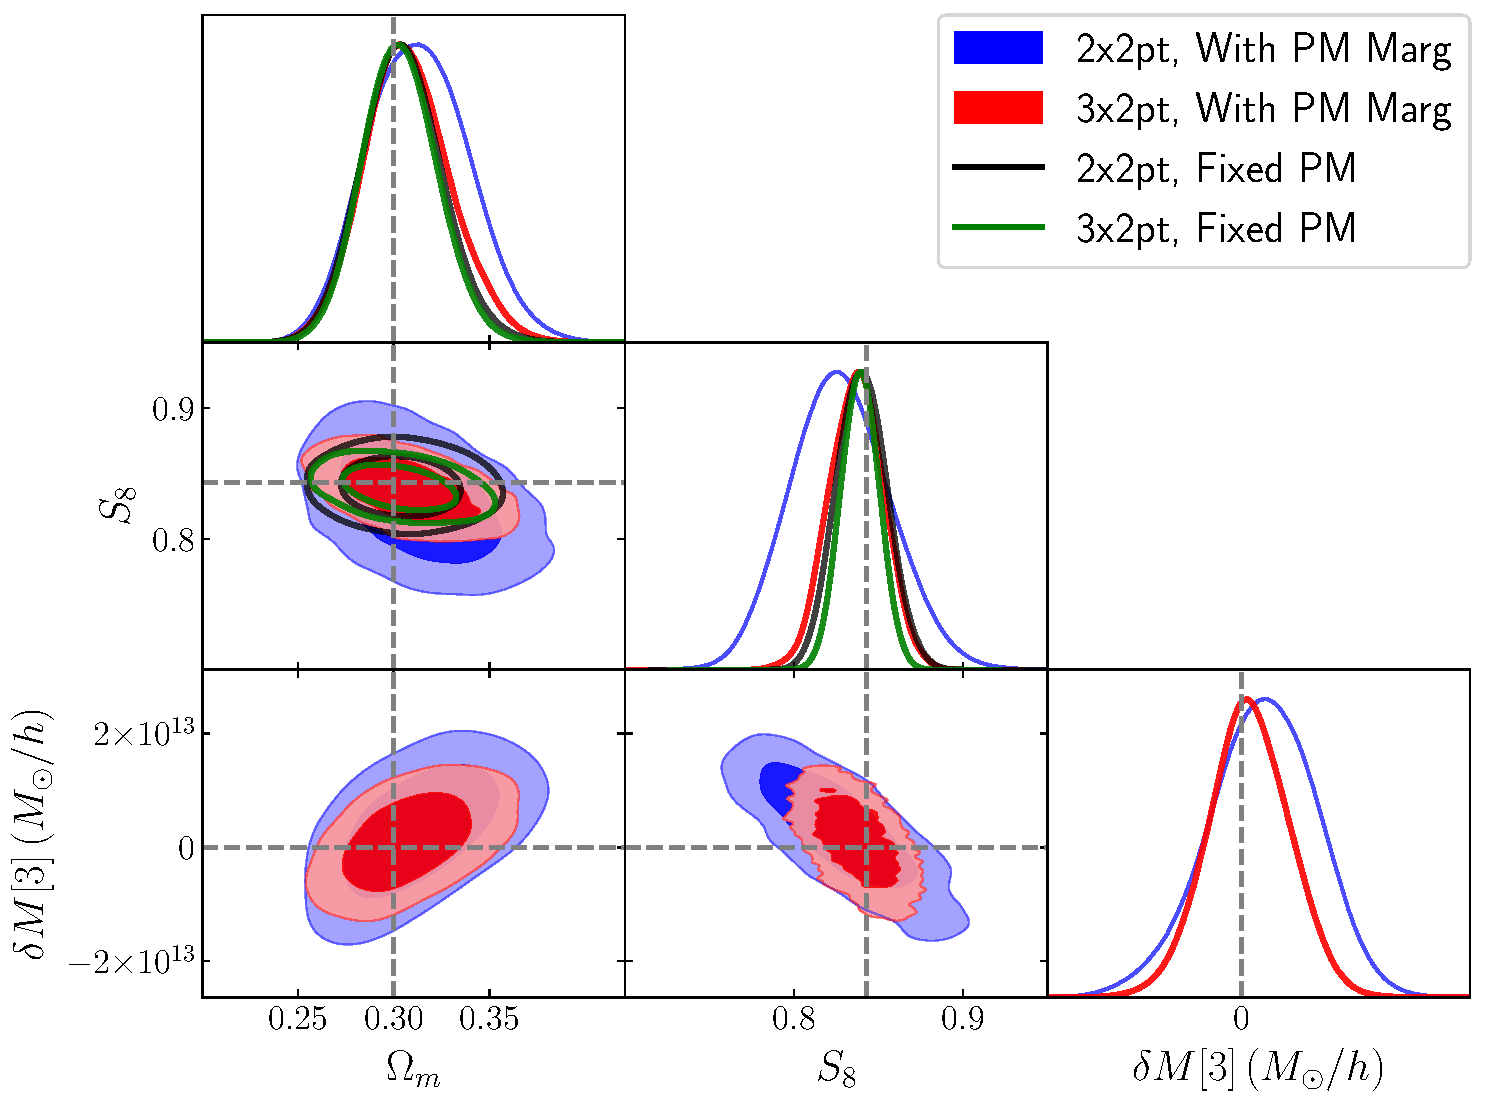
\includegraphics[width=\columnwidth]{figs/PM_constraints_2x2pt_3x2pt.pdf}
\caption[]{Effect of point mass marginalization on the constraining power of $2\times2$pt and $3\times2$pt. We see that the constraining power of $2\times2$pt degrades significantly with point mass marginalization, while for $3\times2$pt the change is minimal. Including the shear-shear correlation  breaks the degeneracy between point-mass (we show PM for third bin, $M_{\rm halo}[3]$) and $S_8$, leading to smaller sensitivity of cosmology constraints on point mass constraints. }
\label{fig:pm_effect}
\end{figure}


\begin{figure}
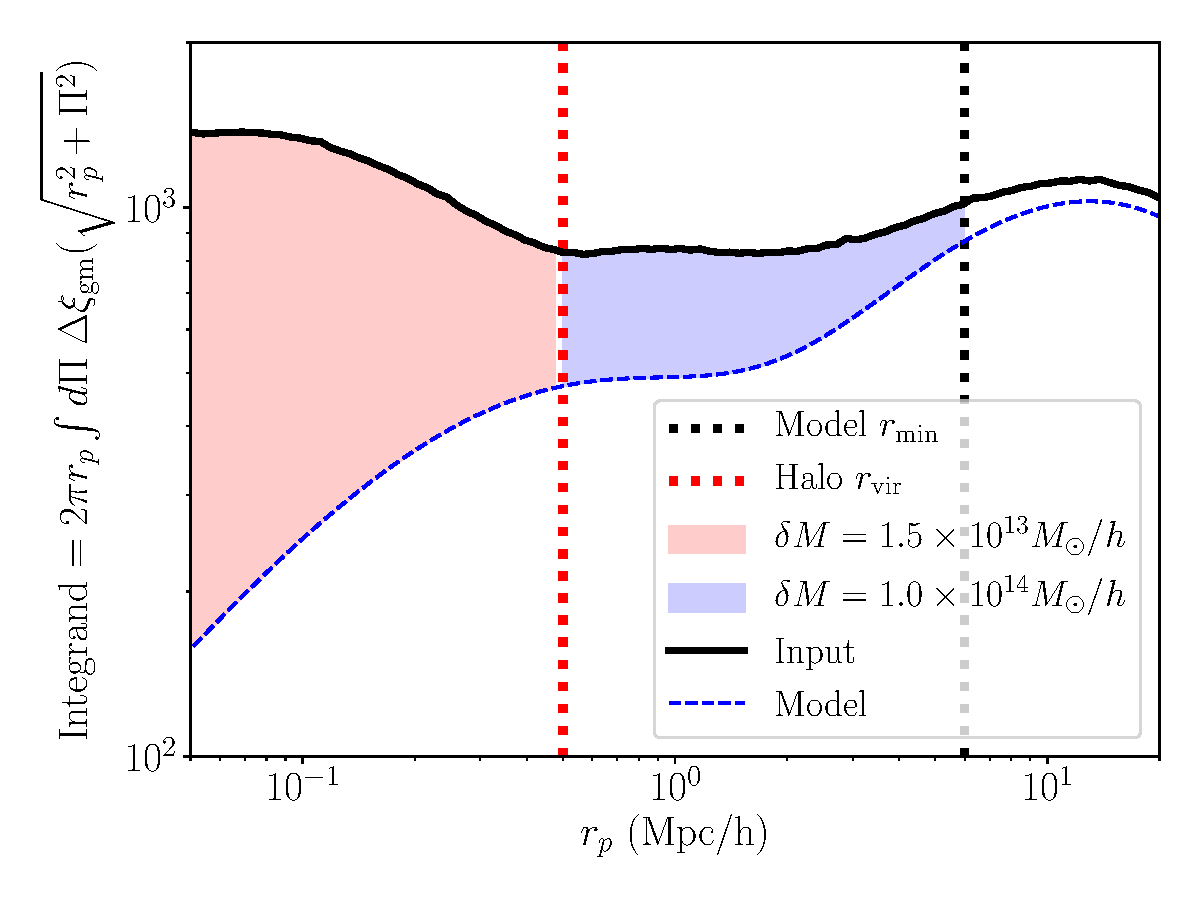
\includegraphics[width=\columnwidth]{figs/PM_contribution_radial.pdf}
\caption[]{We show the contribution to the residual mass shown in Eq.~\ref{eq:pm_halo} from different radial regimes. For simplicity, we assume galaxies to occupy the center of $2.5 \times 10^{13} M_{\odot}/h$ mass halos. The input $\xi_{\rm gm}$ in black solid line is generated using the NFW profile in the 1-halo regime ($r < 0.5 Mpc/h$) and one--loop PT in the 2-halo regime ($r > 0.5 Mpc/h$). We show the contribution to $\delta M$ separately for the 1-halo region (below the red dashed line) and 2-halo regimes (up to the scales of 8Mpc/$h$). We find that the 2-halo regime contributes significantly more than the 1-halo region and the resulting $\delta M$ values is significantly more than the input halo mass of $2.5 \times 10^{13} M_{\odot}/h$. Therefore we can not motivate an astrophysical informative prior on the PM parameters and hence choose a wide prior. 
}
\label{fig:pm_prior}
\end{figure}




% \subsection{Model stress test}
% \subsubsection{Evolution of Point-mass parameters}
The baseline model parameterization assumes the point mass parameter to be constant within each tomographic bin. We test this assumption implicitly in the suite of \buzzard simulations. The datavector measured in N-body \buzzard simulation will capture the effects of evolving point-mass parameters due to the evolution of galaxy-matter correlation within a lens tomographic bin. As we have validated that our scale cuts pass our threshold criteria of bias in cosmological parameters being less than 0.3$\sigma$, we can conclude that the effect of point mass parameter evolution is small. Here we also test this effect explicitly by generating a simulated galaxy matter correlation function using the halo model. We assume a constant HOD of the \redmagic galaxies but include the evolution of halo mass function and halo bias to predict the evolution of galaxy-matter correlation function. The contribution to the PM parameter due to this evolution to each tomographic bin is given by Eq.~\ref{eq:pm_halo}. In Fig.~\ref{fig:pm_evolve}, we show this contribution to each redshift bin by black solid line. We compare this bias with the expected level of uncertainty in the PM parameters by plotting the marginalized constraints on these parameters as shown in Fig.~\ref{fig:pm_effect} for both $2\times2$pt and $3\times2$pt analysis. We see that the uncertainty in PM parameters is significantly greater than the expected bias. 


\begin{figure}
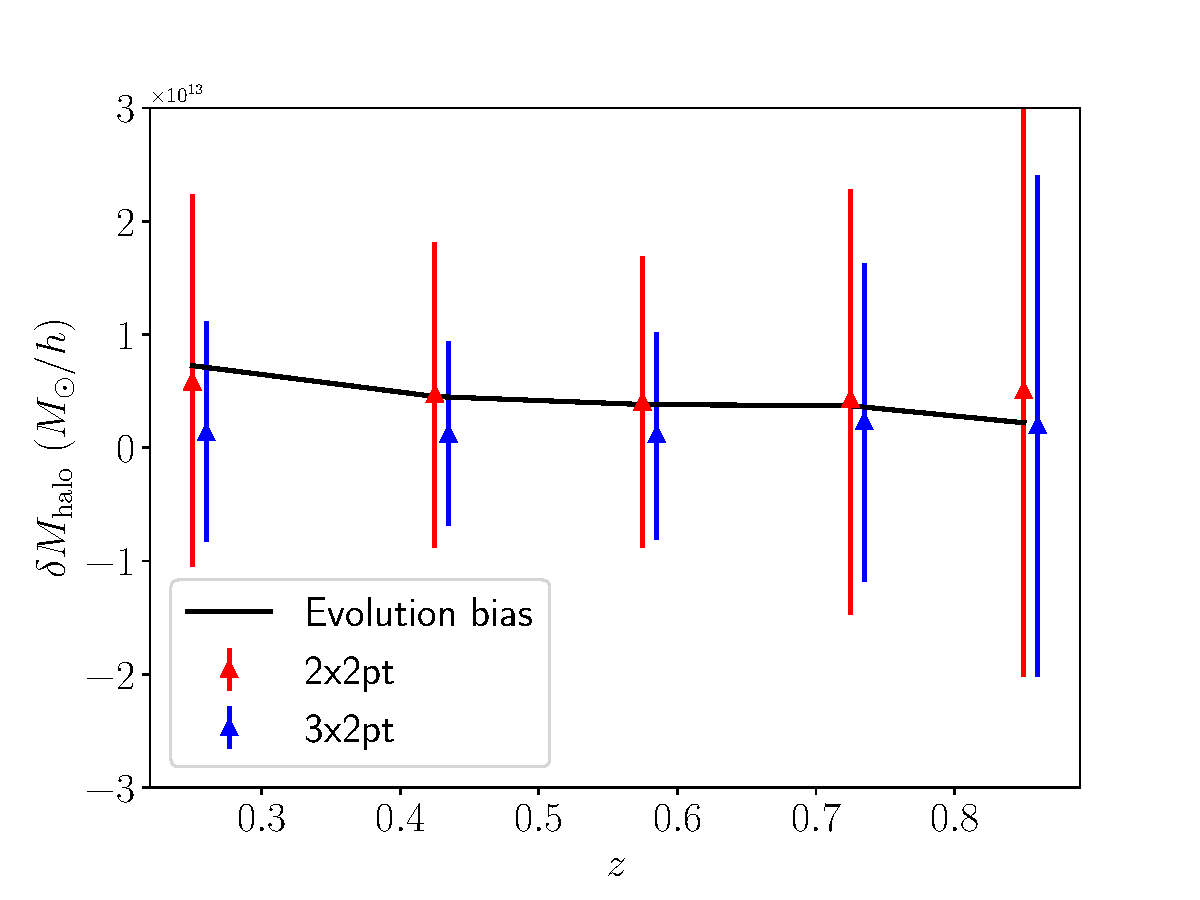
\includegraphics[width=\columnwidth]{figs/PM_evolve_impact.pdf}
\caption[]{We show the effect of the evolution of galaxy matter correlation functions on the PM parameters for each tomographic bin in the black line. The red errorbars show the expected errorbars on PM parameters for $2\times2$pt as shown in Fig.~\ref{fig:pm_effect}. The blue errorbars are the constraints from $3\times2$pt.
}
\label{fig:pm_evolve}
\end{figure}


\section{Datavector residuals}
\IR{In this appendix, we will show the bestfit residuals of the measured correlation functions in simulations and data. In order to get the bestfit PM parameters in order to get good residual, we will sample over these parameters with emcee chain. }

% \subsection{DES Y3}
\begin{figure}
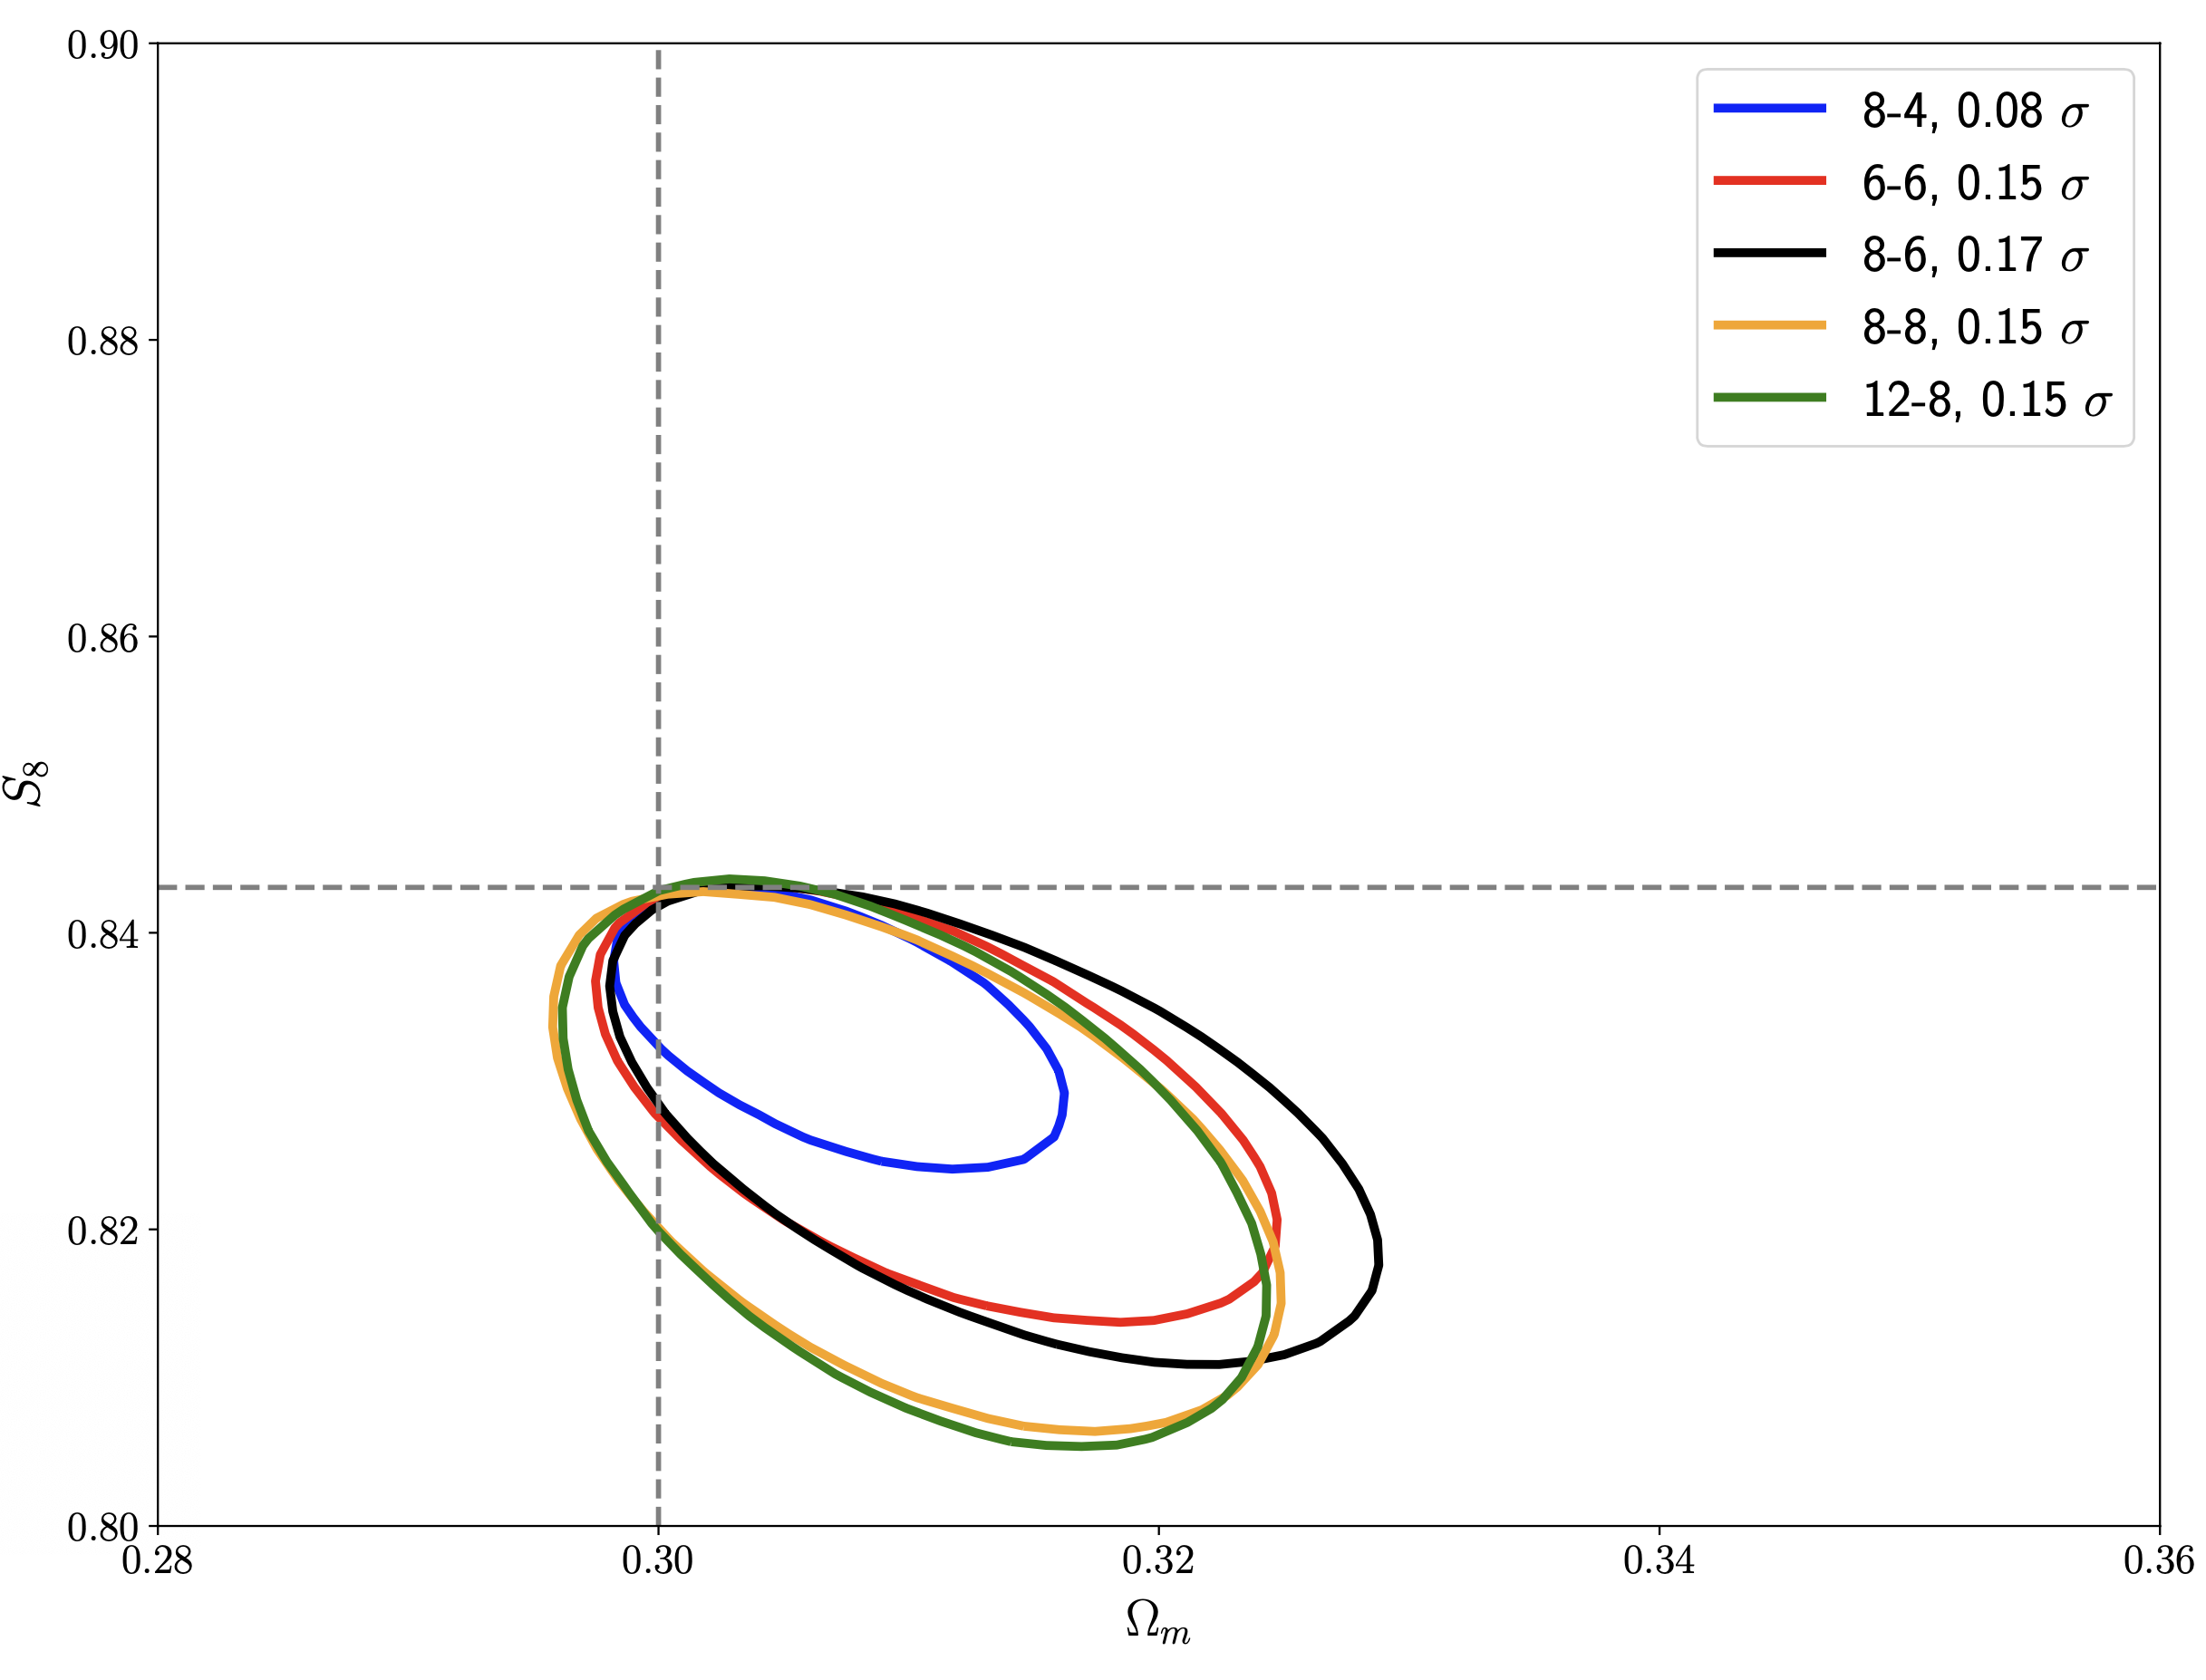
\includegraphics[width=\columnwidth,draft]{figs/temp.png}
\caption[]{Measurements and best-fit of $\wtheta$ and $\gammat$ with DES Y3 data }
\label{fig:data_2pt}
\end{figure}

% \section{Scale cuts validation}\label{app:scale_cuts}
% \subsection{Projection effects}\label{app:projection_effects}
\section{De-correlation parameter constraints}
\blue{Show the constraints on the five $X^{i}_{\rm lens}_i$ parameters. Show how it is fairly similar for atleast the first few tomographic bins. }


\begin{figure}
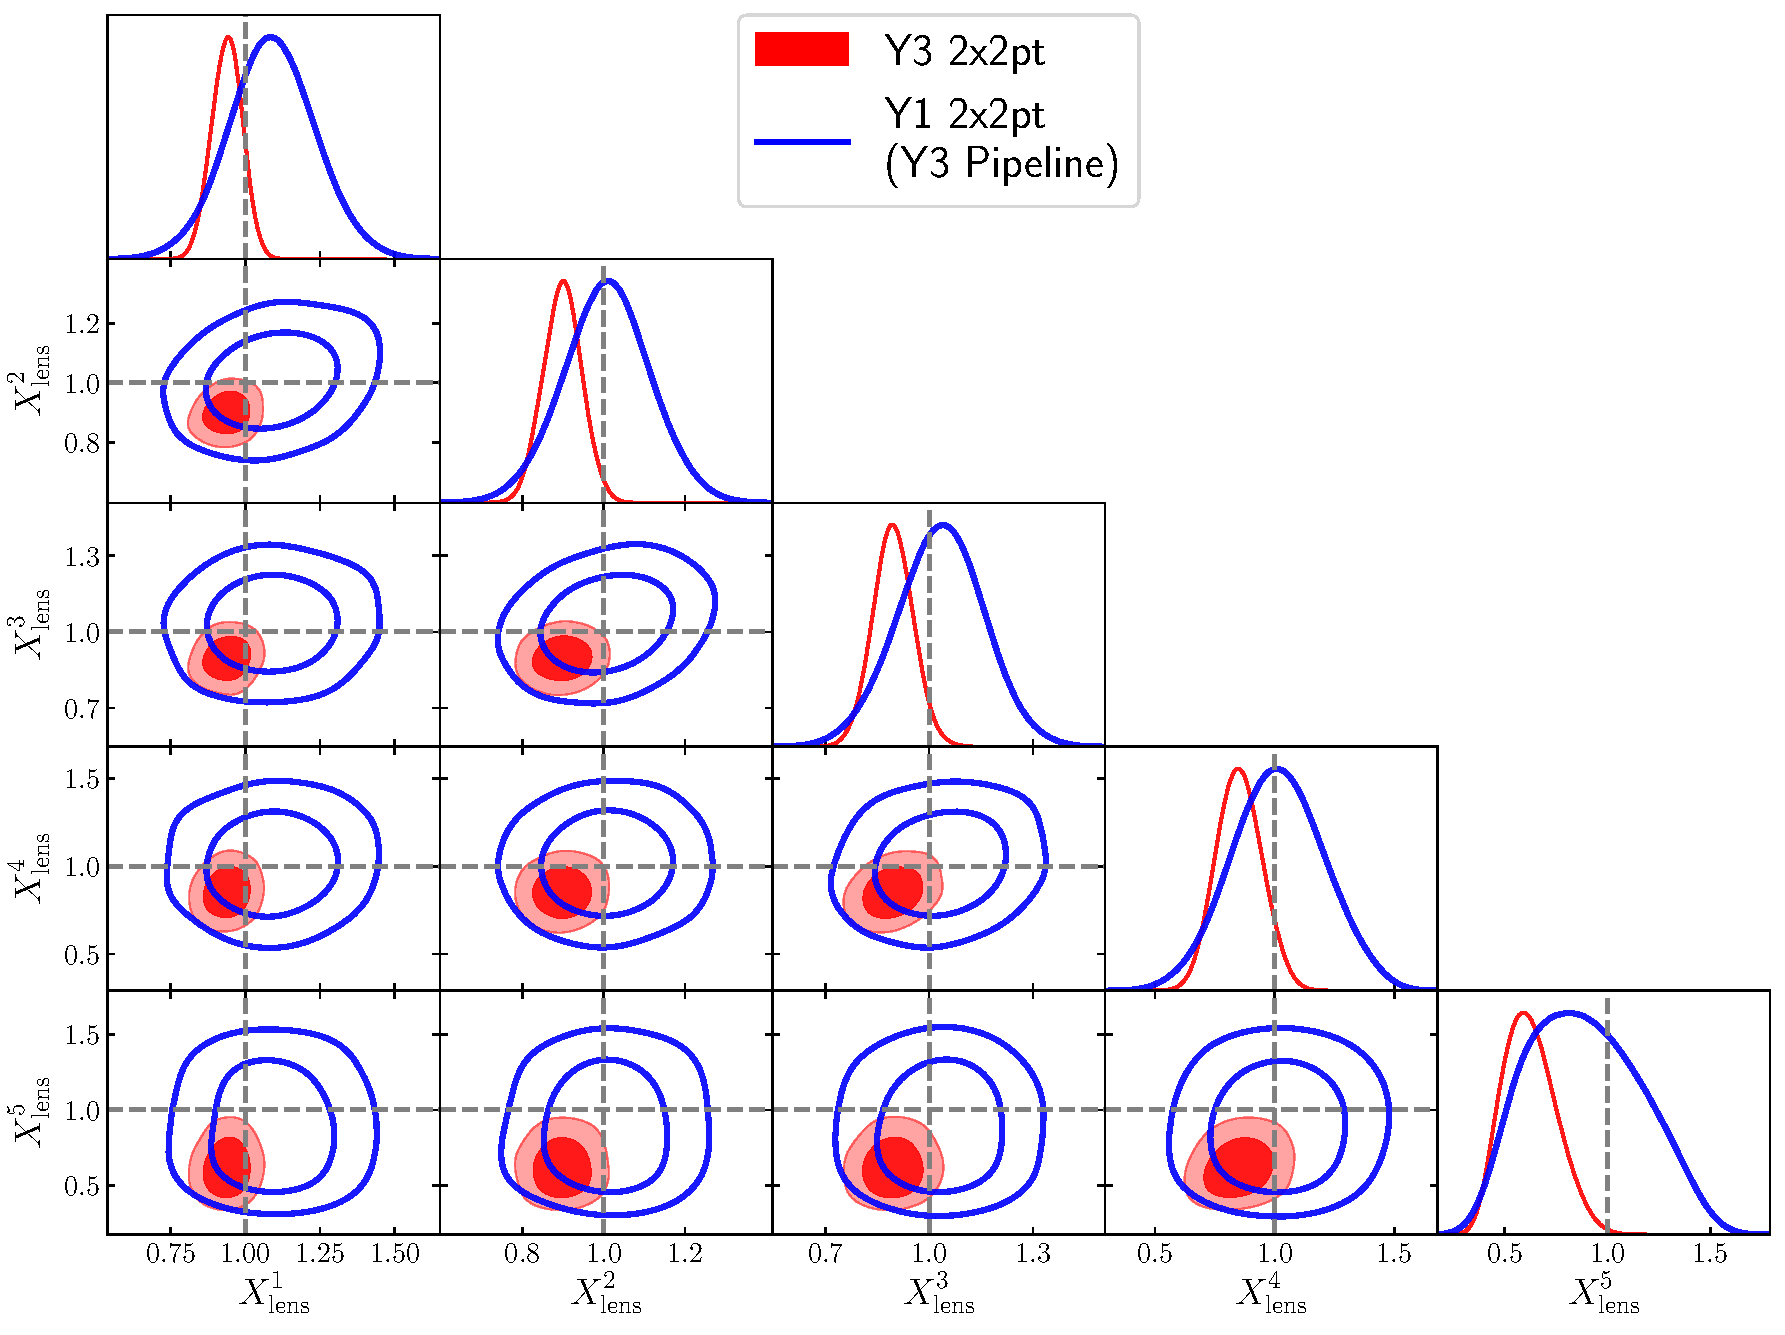
\includegraphics[width=\columnwidth]{figs/Xlens_5_y1_y3_comp.pdf}
\caption[]{Constraints on the de-correlation parameter for each tomographic bin as compared between Y1 and Y3 \redmagic galaxy sample}
\label{fig:pm_evolve}
\end{figure}

\section{BOSS $\times$ $\redmagic$ correlation}
\label{app:bossxrm}
\blue{Describe the methodology to measure and analyze the BOSS cross-correlations. Mention how we split the BOSS into finer bins, show the n(z)'s combined, approximations we make for now. Mention the area overlap and the covariance estimate.}

\section{Halo mass inference}
\label{app:halo_mass}
In this section we detail the methodology to infer the host halo mass of our \redmagic lens galaxy sample from the constraints on galaxy bias parameters and number density. We use halo model framework to make this prediction and parameterize the number of galaxies in a halo of mass $M$ in tomographic bin $j$ be given as $N^{j}_{\rm g}(M) = N^{j}_{\rm{cen}}(M) + N^{j}_{\rm{sat}}(M)$ where $N^{j}_{\rm{cen}}$ is the number of central galaxies and $N^{j}_{\rm{sat}}$ is the number of satellite galaxies. We parameterize these two components as:
\begin{linenomath*}
\begin{align}
    N^{j}_{\rm cen} =  \frac{f^{j}_{\rm cen}}{2} \bigg[1 + {\rm erf}\bigg(\frac{ \log{M} - (\log{M_{\rm min}})^j}{(\sigma_{\log{M}})^j} \bigg) \bigg]  \\
    N^j_{\rm sat} = \frac{1}{2} \bigg[1 + {\rm erf}\bigg(\frac{ \log{M} - (\log{M_{\rm min}})^j}{(\sigma_{\log{M}})^j} \bigg) \bigg] \times \bigg( \frac{M_{\rm h}}{M^j_1} \bigg)^{\alpha^j}.
\end{align}
\end{linenomath*}
Here we have five free parameters, $f^j_{\rm cen}$, $(\log{M_{\rm min}})^j$, $(\sigma_{\log{M}})^j$, $M^j_1$ and $\alpha^j$, that we marginalize over. We can predict the comoving number denstiy ($\overline{n}(z)^j$) and galaxy bias for a given tomographic bin $j$, $b^j_1$, from galaxy HOD as follows:

% \begin{equation}\label{eq:ng}
% ,
% \end{equation}
\begin{linenomath*}
\begin{align}\label{eq:nbar_b1b2}
\nonumber    \overline{n}^j(z) = \int_{0}^{\infty} dM \frac{dn}{dM} N^{j}_{\rm g}(M) \\
\nonumber    b^{j}_1 = \int dz \frac{n^j_g(z)}{\overline{n}^j(z)} \int_{0}^{\infty} dM \frac{dn}{dM} N^{j}_{\rm g}(M) b^{\rm halo}_{1}(M,z)\\
\end{align}
\end{linenomath*}
We use \cite{Tinker_2008} halo mass function ($dn/dM$) and \cite{Tinker_2010} relation for linear halo bias ($b^{\rm halo}_{1}(M,z)$). 

Therefore, Eqs.~\ref{eq:nbar_b1b2} allow us to predict the number density and galaxy bias values. We then sampling these HOD parameters to fit the datavector $\vec{\mathbfcal{D}_H} = \overline{n}^j(z_1)...\overline{n}^j(z_{n}),b^j_1,b^j_2]$ of length $d$ where $\overline{n}^j(z_1)...\overline{n}^j(z_{n})$ are the $n=d-2$ observed comoving number density of \redmagic galaxies as shown in middle panel of Fig.\ref{fig:bias_mass_nbar} and $b^j_1$ and $b^j_2$ are the marginalized mean bias values obtained at our \textit{fiducial} scale cut. For a given set of HOD parameters ($\Theta_{\rm H}$), the theoretical prediction is given by $\mathbfcal{T}_{\rm H}$ and we write our log-likelihood as:
\begin{linenomath*}
\begin{multline}
    \ln \mathcal{L}(\vec{\mathbfcal{D}_H}|\Theta) = -\frac{1}{2} \bigg[ (\vec{\mathbfcal{D}_H} - \vec{\mathbfcal{T}_H}(\Theta_{\rm H})) \, {\mathbfcal{C}_H}^{-1} \,  (\vec{\mathbfcal{D}_H} - \vec{\mathbfcal{T}_H}(\Theta_{\rm H}))^{\rm T} \\ -  \ln(|\mathbfcal{C}_H|) \bigg]
\end{multline}
\end{linenomath*}
In order to account for variation of HOD within a tomographic bin that contributes to the variation on $\overline{n}^j(z)$ within each tomographic bin as seen in Fig.\ref{fig:bias_mass_nbar}, we implement an analytical marginalization scheme. We change the covariance of our datavector $\mathbfcal{C}_H$ as :
\begin{linenomath*}
\begin{equation}
    \mathbfcal{C}_H \to \mathbfcal{C}_H + \alpha_{c} \mathbfcal{I}_D
\end{equation}
\end{linenomath*}
where $\mathbfcal{I}_D$ is a diagonal matrix of dimension $d\times d$ whose diagonal elements equal to 1 from index 1 to d-1, and equal to 0 otherwise. We sample over the parameter $\alpha_{c}$, treating it as a free parameter. 






%%%%%%%%%%%%%%%%%%%%%%%%%%%%%%%%%%%%%%%%%%%%%%%%%%


% Don't change these lines
\bsp	% typesetting comment
\label{lastpage}

% \bibliographystyle{apsrev4-1}
% \bibliography{ref} 

\end{document}

% End of mnras_template.tex